\documentclass{disithesis}
\usepackage[utf8]{inputenc}
\usepackage{amsmath}
\usepackage[dvips]{graphicx}
\usepackage{subfigure}
\usepackage{bm}
\usepackage{graphicx}
\usepackage[export]{adjustbox}
\usepackage{multirow}
\usepackage{times}
\usepackage{epsfig}
\usepackage{amsmath}
\usepackage{amssymb}
\usepackage{rotating}
\usepackage{pdflscape}
\usepackage{url} 
\usepackage{float}
%\usepackage{biblatex} %Imports biblatex package
%\usepackage[round]{natbib}
\usepackage{siunitx}
\usepackage[bottom]{footmisc} 
\usepackage{eurosym}
\usepackage{listings} %Per inserire codice
\usepackage[usenames]{color} %Per permettere la colorazione dei caratteri 
\usepackage{bm} %lettere greche in grassetto
\usepackage{textcomp} %gradi celsius 
\usepackage[dvipsnames]{xcolor}
\definecolor{mgreen}{rgb}{0.1,0.6,0.1}
\definecolor{mpurple}{rgb}{0.3,0,0.4}
\definecolor{morange}{rgb}{0.9,0.3,0}
\usepackage{listings}% http://ctan.org/pkg/listings

\definecolor{dkgreen}{rgb}{0,0.6,0}
\definecolor{gray}{rgb}{0.5,0.5,0.5}
\definecolor{mauve}{rgb}{0.58,0,0.82}

\usepackage{acronym}
\DeclareMathOperator*{\argmin}{arg\,min}

\lstdefinestyle{customc}{
	belowcaptionskip=1\baselineskip,
	breaklines=true,
	%frame=L,
	xleftmargin=\parindent,
	language=C,
	showstringspaces=false,
	basicstyle=\footnotesize\ttfamily,
	keywordstyle=\bfseries\color{mgreen},
	commentstyle=\itshape\color{mpurple},
	identifierstyle=\color{blue},
	stringstyle=\color{morange},
}

\lstdefinestyle{customj}{
    language=Java,
    basicstyle=\small\ttfamily, % needed for "
    %numbers=left,
    %stepnumber=1,
    %frame=single,
    columns=flexible,              % needed because of spaces
    keepspaces=true,               % needed because of spaces
    %numberstyle=\tiny\noncopynumber,    % line numbers shouldn't be copied
    keywordstyle=\color{blue},     % keyword style
    commentstyle=\color{dkgreen},  % comment style
    stringstyle=\color{mauve},     % string literal style
    escapeinside={\%*}{*)},        % if you want to add a comment within your code
    morekeywords={*,...}           % if you want to add more keywords to the set
}

\lstset{escapechar=@,style=customc}

%DIF PREAMBLE EXTENSION ADDED BY LATEXDIFF
%DIF UNDERLINE PREAMBLE %DIF PREAMBLE
\RequirePackage[normalem]{ulem} %DIF PREAMBLE
\RequirePackage{color}\definecolor{RED}{rgb}{1,0,0}\definecolor{BLUE}{rgb}{0,0,1} %DIF PREAMBLE
\providecommand{\DIFadd}[1]{{\protect\color{blue}\uwave{#1}}} %DIF PREAMBLE
\providecommand{\DIFdel}[1]{{\protect\color{red}\sout{#1}}}                      %DIF PREAMBLE
%DIF SAFE PREAMBLE %DIF PREAMBLE
\providecommand{\DIFaddbegin}{} %DIF PREAMBLE
\providecommand{\DIFaddend}{} %DIF PREAMBLE
\providecommand{\DIFdelbegin}{} %DIF PREAMBLE
\providecommand{\DIFdelend}{} %DIF PREAMBLE
%DIF FLOATSAFE PREAMBLE %DIF PREAMBLE
\providecommand{\DIFaddFL}[1]{\DIFadd{#1}} %DIF PREAMBLE
\providecommand{\DIFdelFL}[1]{\DIFdel{#1}} %DIF PREAMBLE
\providecommand{\DIFaddbeginFL}{} %DIF PREAMBLE
\providecommand{\DIFaddendFL}{} %DIF PREAMBLE
\providecommand{\DIFdelbeginFL}{} %DIF PREAMBLE
\providecommand{\DIFdelendFL}{} %DIF PREAMBLE
%DIF END PREAMBLE EXTENSION ADDED BY LATEXDIFF

%\addbibresource{bib.bib} %Import the bibliography file

\begin{document}
	
%

\title{A Solution for Improving\\ Robustness in GNSS Positioning from\\ Android Devices}

\author{Lorenzo Benvenuto}

%%%% If month and year are not the current ones
%%%% \submityear{1997}
%%%% \submitmonth{December}

\technumber{XX}

\maketitle

\begin{addresspage}
{\bf
Dottorato di Ricerca in Informatica ed Ingegneria dei Sistemi\\
Indirizzo Informatica\\
Dipartimento di Informatica, Bioingegneria, Robotica ed Ingegneria dei Sistemi \\
Universit\`a degli Studi di Genova\\[2ex]}

DIBRIS, Univ. di Genova\\
Via Opera Pia, 13\\
I-16145 Genova, Italy\\
{\tt http://www.dibris.unige.it/}\\[2ex]

{\bf
Ph.D. Thesis in Computer Science and Systems Engineering\\
Computer Science Curriculum}\\
(S.S.D. INF/01)\\[2ex]

Submitted by Lorenzo Benvenuto\\
DIBRIS, Univ. di Genova\\
{\tt ....}\\[2ex]

Date of submission:
April 2022\\[2ex]

Title:
A Solution for Improving Robustness of 
GNSS Positioning from Android Devices\\[2ex]

Advisor: Prof. Giorgio Delzanno (DIBRIS), Eng. Tiziano Cosso (Gter)
\\
Dipartimento di Informatica, Bioingegneria, Robotica ed Ingegneria dei Sistemi\\
Universit\`a di Genova\\
{\tt ...}\\[2ex]

Ext. Reviewers:\\
Prof. Paolo Dabove (Politecnico di Torino)\\ Prof. Ferruccio Damiani (Università degli Studi di Torino)
\end{addresspage}


\dedication{ \begin{flushright} \textit{A Giampi: \\l'entusiamo e la passione per il lavoro\\ che mi hai trasmesso durante le giornate \\di rilievo sul campo passate insieme, sono e\\ saranno sempre per me fonte d'ispirazione.} \end{flushright}}

\chapter*{\centering \begin{normalsize}Preface\end{normalsize}}
\begin{quotation}
This research work was carried out as part of an industrial PhD in collaboration with Gter srl\footnote{https://www.gter.it/} and the University of Genoa, DIBRIS departement. The PhD lasted three years (from November 2018 to November 2021) and was funded by Regione Liguria on the POR-FSE 2014-2020 programme (Programma Operativo Regione Liguria, Fondo Sociale Europeo). 
\end{quotation}



\chapter*{\centering \begin{normalsize}Abstract\end{normalsize}}
\begin{quotation}
\noindent
Starting with the Nougat 7.0 version of the Android Operating System released in 2016,  Google has permitted direct access, via the Android development API, to the GNSS raw measurements on Android-based smartphones. This new feature opened a new research field aimed at developing low-cost applications for satellite-based positioning systems. In particular, after the publication of  a white paper from the European GNSS Agency, many authors started to analyse the quality of the raw measurements retrieved from smartphones and compare them with other types of low cost GNSS devices. The main detected issues turned out to be the low quality of the GNSS observables due to the low quality of the hardware (receiver and antenna) mounted in the smartphones. Nowadays raw GNSS measurements support is mandatory on devices that run Android 10 (API level 29) or higher, but unfortunately the support for some of the raw GNSS measurement fields (e.g. pseudorange rate, ADR, AGC) is optional and can vary based on the type of GNSS chipset installed on the device. Furthermore, not all the smartphones present on the market support double frequency or multi-constellation.

In this thesis we present a solution for improving the robustness of GNSS positioning in Android devices in real time, that combines an acquisition phase performed in a dedicated Android app (thus working on the edge) and a processing phase, based on a modified version of the open source library RTKLIB, performed on dedicated servers. 
The processing phase performed on the smartphone is aimed at cleaning, filtering, organizing and delivering the data acquired via the GNSS raw data library. 
The server-side processing phase applies an improved version of the RTK library.
Our version provides an additional interface for processing different format of GNSS data (in particular a new one defined for GNSS measurement from Android devices) and a method to mitigate in real-time the multipath effect on the collected data. 

We will focus our attention on the architecture of the proposed solution (Android endpoints and processing server), on the proposed improvement of the GNSS positioning procedure, and its implementation in our version of the RTKLIB library, and on preliminary results obtained by the resulting system.
\end{quotation}

%\begin{citetext}{?}
%?
%\end{citetext}

\tableofcontents	
\listoffigures
\listoftables
%\chapter[State of art]{\begin {Huge}\textit{\bf{State of art}} \end{Huge}}

\chapter[Introduction]{\centering \begin{normalsize} \begin{Huge}
			Introduction
		\end{Huge} \end{normalsize}}
\label{ch:intro}
\section{Background and Motivations}
%Motivations and a concise description of the goals of the thesis
Global Navigation Satellite System (GNSS) refers to a constellation of satellites that broadcast their positioning and timing data to GNSS receivers. The most famous GNSS is NAVSTAR GPS  installed by the U.S. Department of Defense in the '70s. A receiver estimates the time it takes for each signal to travel from the GNSS satellite antenna to the user's antenna. The receiver can then use four satellite data to determine its location. 

Modern smartphones are equipped with GNSS receivers, e.g. to receive GPS data. Cellular location, provided by phone carriers, can assist the satellite-based location process (Assisted GPS). Indeed, software on smartphones feed raw cellular location data to the GPS receiver, which periodically switches between GPS data and cellular location to get a very close approximation in real-time. Internet routing data can also be used as additional location data. 

In May 2016, during the ``Google I/O” conference, Google released an Application Programming Interface (API) to give Android developers access to GNSS raw measurements such as carrier phase, code measurements and navigation messages. 
As stated in the white paper \cite{GSA_wp:2016} of the GNSS Raw
Measurement Task Force, coordinated by the European GNSS Agency (GSA), this new feature of the Android API 
offered new research directions and, more in general, new opportunities.  
In particular, GNSS raw measurements can be used to optimise  multi-GNSS and multi-frequency solutions, to select the satellites based on their performance,  to transfer processing techniques from GNSS receivers to smartphones, to combine GNSS raw data with data of other sensors that are available in smartphone and to enable testing and post-processing analysis.

From a technical point of view, the use of GNSS raw measurements posed several challenges for both GNSS experts and Android developers.
Indeed, on one hand GNSS standard formats, such as RINEX or NMEA, are not natively available on the Android platform. On the other hand Mobile app developers are in general not familiar with the complex algorithms and libraries used in GNSS positioning.

The GSA white paper \cite{GSA_wp:2016} addressed the gap between the two fields providing useful information, e.g. for deriving the pseudoranges from Android. 
This important work opened a new research field aimed at developing low-cost applications for satellite-based positioning systems. 
In particular, after its publication many authors started to analyse the quality of the raw measurements retrieved from smartphones and compare them with other types of low cost devices. The main detected issues turned out to be the high noise of the GNSS observables. Indeed, smartphones are equipped with cellphone-grade GNSS chipsets and antennas, which have on average very low gain resulting in low and irregular Signal to Noise Ratio (SNR) \cite{Zangenehnejad:2021}. For this reason smartphone positioning is very challenging, especially in harsh environments such as urban areas that are more vulnerable to the multipath and other interferences \cite{Angrisano:2022}.

Nowadays raw GNSS measurements support is mandatory on devices that run Android 10 (API level 29) or higher, but unfortunately the support for some raw GNSS measurement fields (e.g. pseudorange rate, ADR, AGC) is optional and can vary based on the type of GNSS chipset installed on the device. Furthermore, not all the smartphones present on the market support double frequency or multi-constellation.
For this reason, finding a robust use of GNSS raw measurements is still a topic of interest for the research communities working on GNSS and mobile computing.
%
%\section{Overview of the State of the Art}
%Existing works (or Background)}
The possibility to access GNSS raw measurements from Android  has changed the concept of precise positioning with portable devices. Several studies have been conducted to verify the feasibility \cite{Humphreys:2016} and positioning accuracy \cite{Pesyna2014, Zhang:2018} of smartphones for different purposes, from urban \cite{Masiero2014, adjrad2018} to pedestrian positioning applications
\cite{presti2017, Fissore2018}, always facing problems related to the use of the Google API and to the filtered measurements provided by the GNSS chipset.
In \cite{realini2017}, the authors demonstrated that it is possible to reach a decimeter level of accuracy
in terms of positioning performances following the post-processing approach, made by
double differencing raw smartphone observations. Meanwhile, the authors of \cite{Dabove2019b} first focused
their attention on single-base RTK positioning and then demonstrated the possibility
of obtaining a centimeter-level accuracy through the use of NRTK corrections \cite{Dabove:2019}.
%
Concerning  apps that can be used for logging GNSS raw data, 
in 2016 Google released the open source GnssLogger to record measurements in csv format.
Other apps such as  Geo++ RINEX Logger,  RinexON, GalileoPVT, and GNSS/IMU Android Logger can produce  GNSS raw measurements and sensor data in different standard formats including the 
RINEX format.
%Differently, from the above mentioned applications, our Android app  can be viewed as the edge component for our RTK-based processing system.
%Indeed, we have defined an ad hoc format for the raw measurement 
%in which the entire set of observables of an entire epoch is packaged in a single message and sent to the multipath mitigation procedure. Porting 
%our extension of RTKLib to Android is a possible future direction to explore in the style of  recent projects such as RTKLibDroid and RtkGps.

 Concerning the hardware, early smartphones only provided single-frequency and mostly GPS-only observations. In 2017, the Samsung S8 and Huawei P10 smartphones were released as the first multi-GNSS devices which are able to track carrier-phase measurements. However, in May 2018, the Xiaomi Mi 8 equipped with the new Broadcom BCM47755 GNSS chipset was released as the world’s first dual-frequency GNSS smartphone, i.e. added with L5 for GPS and E5a for Galileo \cite{Zangenehnejad:2021}. It can be also regarded as a great millstone in smartphone positioning as it provides the users with an opportunity to make ionospheric-free linear combination between observations of two frequencies to eliminate the ionosphere effect.

 In \cite{Robustelli:2019} authors conducted some positioning tests using the Xiaomi Mi8 devices in different multipath conditions showing that the positioning quality is definitely degraded as the multipath effect increases. In particular, they show that, if a relative positioning is considered, under low multipath conditions the obtained planimetric accuracy is about 1 m, while under high multipath conditions the planimetric accuracy is degraded to 2 m. In this thesis work some positioning tests were conducted and discussed with the aim of having an assessment of the position quality from Android devices. Similar results to the ones exposed by previous researches in terms of positioning accuracy were found. Some positioning outliers, probably due to the multipath effect, were also observed. Those outliers compromised then the overall solution robustness making GNSS positioning from smartphone not very affordable.

\section{Research Question}
%
As mentioned before, the multipath effect is probably the major source of error in urban scenarios affecting the positioning quality.
A series of tests carried out with smartphones equipped with dual frequency receivers (Broadcom and Snapdragon chipsets) 
confirmed this hypothesis experimentally. 
Multipath is also a serious problem for the application 
of GNSS positioning algorithms that use raw measurements.

Our research question is whether multipath mitigation techniques used for GNSS receivers can be applied to RTK positioning in Android devices. RTK positioning is a class of algorithms that employ correction codes received from base stations.
They are particularly interesting since they can reach centimetric accuracy without the need of cellular or Internet data.
More in particular, in this setting our goal is to investigate different types of heuristics to increase robustness, in terms of precision and accuracy, of RTK positioning in Android devices.
%

\section{Contributions}
%

\subsection*{A Multipath Mitigation System for Android Smartphones}
Our first contribution is the design and implementation of a 
prototype system for applying multipath mitigation heuristics in RTK positioning with GNSS raw measurements.
The proposed system is based on a pre-processing phase performed in a dedicated Android App (thus working on the edge) and on a real time processing phase, based on a modified version of the open source library RTKLIB, performed on a dedicated server.
The performance of the resulting system, including client-server latencies, is comparable to RTK positioning procedures for GNSS receivers and Assisted GPS computing procedure. It is important to notice that both other solutions require network communication steps too.

%
The data acquisition phase performed via an Android App developed during the PhD work is aimed at cleaning, filtering, organizing and delivering the data acquired via the GNSS raw measurements library. The App is in charge of collecting satellites data of a given epoch, namely raw observations of different satellites and frequencies, converting them into a special message format, and sending the resulting message to the processing server.
The App has several other functionalities including that of receiving and visualizing the position inferred by our algorithms and of providing options to control the acquisition phase, e.g. flags to enable/disable duty cycle and real time plot of SNR parameter.

The server-side processing phase exploits an improved version of the RTKLIB library, enabling RTK positioning from smartphones and increasing the solution robustness by means of multipath mitigation. 
In order to make RTKLIB working in real time with smartphones, a new API's for processing GNSS data in the format defined for data collection was added to the original library.
Concerning the multipath mitigation, the so-called MDP (Multipath Detection Parameter) algorithm conceived and patented by Gter, was implemented in the RTKLIB version adopted in this work. This algorithm, performs multipath detection and mitigation in real time for single frequency GNSS receivers.
During the thesis work the MDP algorithm was improved and adapted for working with GNSS observables from Android devices. The main idea here is to weigh observations of each satellite data with parameters associated to multipath (MDP variable) and signal noise (SNR) error.
The resulting weights are used to tune the RTKLIB positioning algorithms in order to assign low weights to unreliable observation.
The algorithm has several possible configuration parameters and operating modes. In particular, one of the biggest improvements of our algorithms is in the adoption of adaptive thresholds that are inferred via statistical analysis of collected data.
%
\subsection*{Experimental Validation}
%

The procedure described above was tested and validated using two different datasets:
\begin{itemize}
\item A static acquisition with multipath effect induced
\item A kinematic acquisition
\end{itemize}
For both the case studies several combinations of the MDP algorithm configuration parameters were tested.
The preliminary results obtained with the proposed application and mitigation algorithm are very interesting.
More specifically, improvements in positioning accuracy were noted, especially for the period of induced multipath, meaning that the MDP algorithm is suitable for the mitigation of such effect. Furthermore in the solution obtained with the MDP algorithm application some positioning outliers are eliminated, and consequently the solution's robustness is increased. 
The results obtained are then very promising nevertheless many further tests and processing are needed both for continue validating the obtained results, which shall be supported by a stronger statistics, and for continue improving the MDP algorithm performances. 
%
\subsection*{Collected Datasets}
Finally, a further contribution of our work consists in the creation 
of large repository of surveys having both GNSS raw measurements from Android smartphones and observables from professional GNSS receivers, in the different scenarios described in detail in the thesis, hence potentially replicable. The datasets will be made available to the research community to foster future collaborations and advancements in the field.
%
\section{Plan of the Thesis}
In the thesis we will focus on the architecture of the proposed solution (Android endpoints and processing server) and on the proposed improvement of the GNSS positioning procedure. In Chapter \ref{ch:gnss} we will give some preliminary notions on GNSS positioning. In Chapter \ref{ch:SoA} we will presents the key points of GNSS raw measurements in Android and of the RTKLIB open source library. In Chapter \ref{ch:quality_analisys} we will describe quality assessment tests performed using dual frequency smartphone and other GNSS receivers. In Chapter \ref{ch:service_devel} we will illustrate the design and implementation of our multipath mitigation systems. In Chapter \ref{ch:mdp_results} we will discuss experimental results obtained via a series of full track surveys. In Chapter \ref{ch:conclusions} we will address some conclusions as well as present and future directions of our work.





\chapter[GNSS Overwiev]{\centering \begin{normalsize} \begin{Huge}
			GNSS Overwiev
		\end{Huge} \end{normalsize}}
\label{ch:gnss}

The acronym GNSS\footnote{Global Navigation Satellite Systems} refers to all the satellite systems which allow to define the position of a terrestrial point through the emission of radio signals. The most famous GNSS is NAVSTAR GPS\footnote{NAVigation Satellite Timing And Ranging Global Positioning System}; it was the first installed by USA Department of Defense in 1970s and it is the most widespread. Afterwards, the Russian Federal Government decided to invest in satellite positioning by developing the GLONASS\footnote{GLObal'naja Navigacionnaja Sputnikovaja Sistema} system. In the last years, other countries started to develop their own systems: the European Union presented Galileo and EGNOS\footnote{European Geostationary Navigation Overlay System}, Japan is developing QZSS\footnote{Quasi-Zenith Satellite System}, China is working on BeiDou and India on IRNSS\footnote{Indian Regional Navigational Satellite System}.

Many textbooks present the theory of the GNSS (e.g. \cite{hoffmann2008, Teunissen, Seeber:2003}), and it is not the main purpose of this dissertation to provide a fully detailed description of all these aspects. Nevertheless, this chapter resumes in a non exhaustive way the main concepts on the GNSS positioning with the aim of giving the reader the basic elements to understand the rest of the thesis work.
%Satellite technology is currently named GNSS, referring to the satellites' multi-constellations system
%providing global coverage.


\section{GNSS principles}

GNSS is used to determine the position of a receiver by means of constellations of multiple artificial satellites, knowing the positions of the satellites, namely the ephemerides. The determination of the receiver position, i.e. latitude, longitude and height, relies on the calculated distance from several satellites. Theoretically, from a purely geometrical point of view, the minimum needed number of satellites is three, to solve the three unknowns system. The signals of each satellite allow the user to measure the distance between the receiver and the satellite. This operation is based on two clocks, one on the satellite and one on the receiver, which have totally different time scales: in fact, the receiver's clock starts when the receiver is switched on. This effect is called \textit{synchronisation offset} $\delta t$ and it has to be estimated. Moreover, as widely known, the satellites are equipped with atomic clocks which can be synchronized to the level of nanosecond, but GNSS receivers are typically equipped with less expensive crystal clocks. The synchronisation between the clocks has to be estimated with high precision: a synchronization error of 1 $\mu s$ could lead to a position error in the order of 300 meters. The satellite-receiver distance is calculated on the basis of the signals time of travel $ \tau_{sat,rec}$, using the speed of light $c$:

\begin{equation}
	\rho = c \cdot \tau_{sat,rec}
	\label{eq:pseudorange}
\end{equation}

where $\rho$ is called \textit{pseudorange} because it is affected by synchronisation offset. The introduction of $\delta t$ leads to a system of four unknowns, which must be solved by means of four equations. Thus, to overcome the synchronization problem, a fourth satellite is needed. As a matter of facts, having more than four satellites will not result in a more precise solution, but will just increase the control on the observations, thanks to redundancy.

\section{GNSS segments}

A GNSS is composed by three segments:
\begin{itemize}
	{\item[-] space segment},
	{\item[-] control segment},
	{\item[-] user segment}.
\end{itemize}

\textit{The space segment} consists of many constellations of satellites that are placed above the Earth in nearly circular orbital planes. There are three different orbit altitudes: low Earth orbit (LEO), medium Earth orbit (MEO), and geostationary Earth orbit (GEO) satellites.
The relation between orbit altitude and Earth circulation period is fixed. LEO satellite are located at an altitude of under 2000 km and circulate the Earth in the range of 95 to 120 min. MEO satellites are located at an altitude of 5000 to 20000 km and take about 6 h to circulate the Earth. The altitude of GEO satellites is fixed at 35786 km, in which they exactly match the Earth rotation speed (i.e. circulate the Earth once in 24 hours) and remain exactly at the same point from the Earth view. Each satellite is equipped with devices that are used for navigation or other special tasks. The satellite receives, stores, and processes transmitted information from a ground control center. In order to be recognised, satellites have various identification systems, such as the launched sequence number, the orbital position number, and the system specific name.

\textit{The control segment} is responsible of controlling the whole
system including its deployment and maintenance, tracking of the satellites in their orbits and the clock parameters, monitoring of auxiliary data, and upload of the data message to the satellites. The control segment is also responsible for data encryption and service protection against unauthorized users. Moreover, tracking stations located around the world coordinate the activities for controlling and monitoring the system using bidirectional communication between GNSS satellites.

Finally, the \textit{user segment} consists of all the users equipped with passive receivers, i.e. GNSS receivers and antenna, able to acquire, decode and record the signals coming from satellites.

Figure (\ref{FIG:GNSSsegments}) shows a scheme of GNSS segments.

\begin{figure}[ht] 
	\centering
	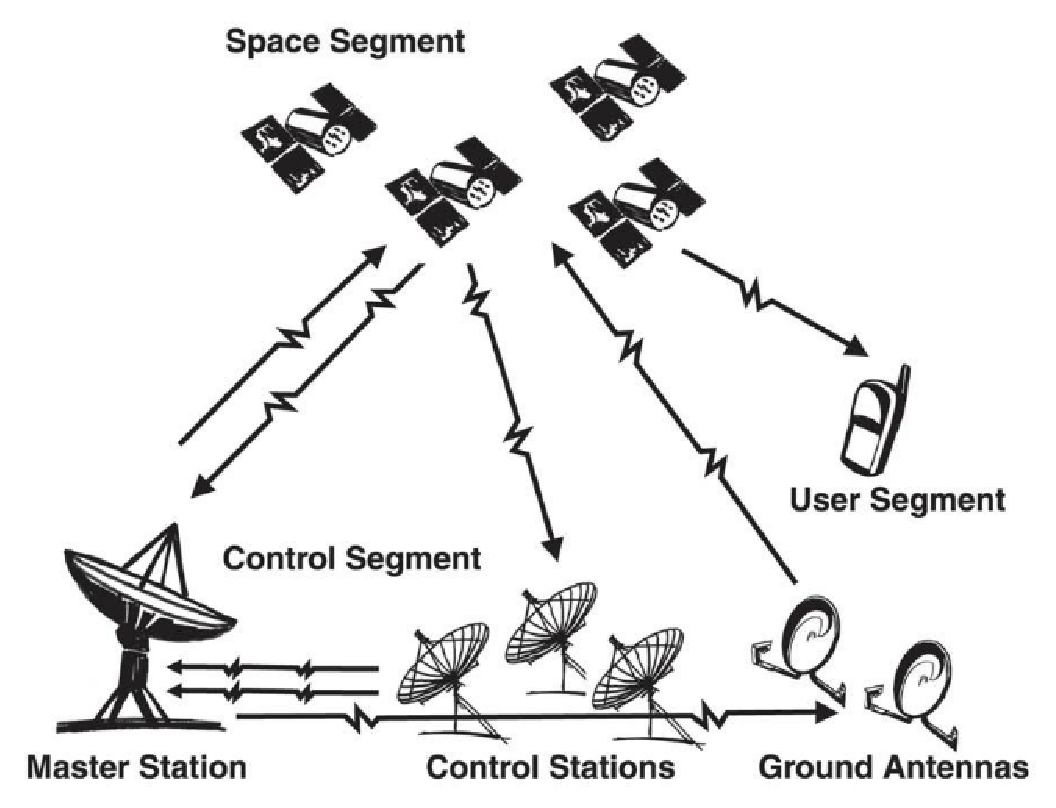
\includegraphics[scale=0.5]{fig/GNSSsegments.eps} 
	\caption{GNSS segments}
	\label{FIG:GNSSsegments} 
\end{figure}

\subsection{GPS}

The NAVSTAR Global Positioning System has been developed by the U.S. Department of Defense for military purpose; the first satellite was launched in 1977 and the system reached its full operational capacity in 1995. Then, in 2000, the U.S. Congress made the GPS available for civilians too, thus, since that time, civilians can access GPS service worldwide free of charge.
The space segment of GPS consists of 24 active MEO satellites, at an altitude of 20200 km, distributed in six equally spaced orbit planes with inclination of $\ang{55}$ on to the Equator. Each satellite circulates the Earth in a period of 12 sidereal hours. The constellation allows the visibility of at least four satellites everywhere and in every time with an elevation of more than $\ang{15}$ on the horizon; this is the minimum requirement for retrieving of the position, but often a higher number of satellites (7 or 8) can be seen. 


%\textcolor{blue}{It is important to underline that the geometrical collocation of the satellites strongly influences the positioning accuracy. The effect of satellites geometry is usually expressed by the DOP\footnote{Dilution Of Precision} index. The different parameters to quantify the goodness of the geometrical configurations are called PDOP\footnote{Position DOP}, HDOP\footnote{Horizontal DOP}, VDOP\footnote{Vertical DOP}, TDOP\footnote{Time DOP} and GDOP\footnote{Geometric DOP}. In particular GDOP index measures the overall accuracy:}
%%spostare dopo sta parte??
%
%\begin{equation}
%GDOP = \sqrt{{\sigma_{x}}^{2}+{\sigma_{y}}^{2}+{\sigma_{z}}^{2}+{\sigma_{t}}^{2}}
%\label{eq:GDOP}
%\end{equation}
%
%where $\sigma$ is the root mean square of the 3D coordinates and time.

The control segment consists of a network of monitoring stations spread around the world mainly along the Equator, and a master control station located in Colorado Springs (Colorado, USA).

The GPS signal is based on the fundamental frequency:

\begin{equation}
	\begin{matrix}
		f_{0} = 10.23 & [\unit{MHz}]
	\end{matrix}\\
	\label{eq:f0GPS}
\end{equation}

whose stability and accuracy is guaranteed by the atomic clocks on the satellites. 
The satellites send signals at three-band frequencies, L1, L2 and L5, obtained as multiple of the fundamental frequency, which represents the carrier component.

\begin{equation} 
	\begin{matrix} 
		f_{1} = 154\cdot f_{0} = 1575.42 & [\unit{MHz}]\\ 
		f_{2} = 120\cdot f_{0} = 1227.60 & [\unit{MHz}] \\
		f_{5} = 115\cdot f_{0} = 1176.45 & [\unit{MHz}] \end{matrix} 
	\\
	\label{eq:f12GPS}
\end{equation}

The two corresponding wavelengths are:

\begin{equation} 
	\begin{matrix} 
		\lambda_{1} = 19 & [\unit{cm}]\\ \lambda_{2} = 24  & [\unit{cm}]\\
		\lambda_{5} = 26  & [\unit{cm}]\end{matrix} 
	\\
	\label{eq:lambda12GPS}
\end{equation}

The information content in a GPS signal is introduced modulating two different codes on the carrier wave. These codes are specific for each satellite and are called codes of \textit{Pseudo-Random Noise} (PRN). The L1 frequency is designed to be modulated with two PNR codes, for civil and military use, while the L2 frequency is modulated just with the military code. There are two types of codes on the carrier signals: \textit{Coarse Acquisition} (C/A) code and \textit{Precise} (P) code. The C/A code is modulated on the L1 carrier; it is a binary sequence of 1023 bit generated at the
frequency of 1.023 MHz, a period of 1 ms and a wavelength of 293.1 m. The C/A code contains the time information on the transmission of the signal according to the satellite atomic clock, and it is also used to identify the satellites, because each satellite has its own C/A code.
The P code is modulated on both the L1 and L2 carriers; it is a more complex binary sequence than C/A, generated at the frequency of 10.23 MHz, a period of 7 days and a wavelength of 29.3 m. The actual P code is not directly transmitted by the satellite, but it is modified by a Y code, which is often referred to as the P(Y) code. The P(Y) code, which has similar properties to the P code, is not available to civilian users and is primarily used by the military: in other words, the P(Y) code is classified. 

%The P code contains the time information according to the satellite atomic clock when the signal was transmitted as C/A code, except that it has a ten times higher resolution.
The GPS navigation message is transmitted in both L1 and L2 frequencies at a very low rate (50 bps). The navigation message allows the users to know the satellites positions in real time and it contains the broadcast ephemerides, the predicted model coefficients of the satellite clocks, information about the GPS state system and an approximate model of the ionosphere.

The GPS coordinates are transformed from Cartesian geocentric to Geodetic and expressed in the WGS84\footnote{World Geodetic System} reference frame. The reference time of GPS is GPS time (GPST), the time scale implemented by the atomic clocks on the GPS ground control segment and the GPS satellites themselves. GPS time started at 00:00 h UTC on 6\textsuperscript{th} January 1980 and since it is not affected by leap seconds, GPS is now ahead by 17 seconds on UTC.



\subsection{GLONASS}

GLONASS has been developed by Russian Federal Space Agency and Ministry of Defense since 1970.
The first GLONASS satellites were launched in 1984; in 1993 the orbital constellation of GLONASS
reached 12 satellites. In 2011, GLONASS became fully operational with a complete constellation of 24 satellites. Likewise GPS, GLONASS has been developed mainly for military purpose, but it is now available for civilian usage too. 

The GLONASS space segment consists of 24 satellites in three orbital planes at the altitude of 19100 km, with $\ang{64.8}$ of inclination with respect to the Equator, and divided by $\ang{45}$ in latitude. Among these satellites, 21 are active and the other three are used as spares. This constellation ensures at least five visible satellites at any point in the Earth.

The control segment consists of the Ground-based Control Complex (GCS) in Krasnoznamensk and it is connected with 8 Command Tracking Stations (CTS) distributed across the country.
GLONASS gives two different signals: \textit{Standard Precision} (SP) and \textit{High Precision} (HP). Just the SP signals are available for civil users, and the frequencies of the signals are:

\begin{equation} 
	\begin{matrix} 
		f_{1} = 1602 + n \cdot 0.5625 & [\unit{MHz}]\\ f_{2} = 1246 + n \cdot 0.4375 &[\unit{MHz}] \end{matrix} 
	\\
	\label{eq:f12GLONASS}
\end{equation}

where $n$ is the number of the channel; it means that each satellite transmits on a particular frequency. The signals are modulated by C/A code and P code; the C/A code is only modulated onto L1, while P code is modulated onto L1 and L2. Besides L1 and L2 carriers, GLONASS satellites transmit signals in L3 carrier frequency (1204.704 MHz). This third frequency increases the reliability and accuracy and it will be especially used for safety applications

The navigation message includes information about the satellites orbits, satellites status, correction data, and the almanac data about all satellites within GLONASS constellation. In addition, it includes the
correction to GLONASS time with respect to UTC and the time difference between GLONASS time and GPST. The GLONASS reference time is GLONASS time (GLONASST), which is synchronized within 1 ms with UTC time, with a constant offset of three hours. GLONASS coordinates are expressed using PZ-9016 reference frame.

\subsection{Galileo}

In 2002, the European Union (EU) and European Space Agency (ESA) agreed to introduce their own GNSS, called Galileo, as an autonomous, alternative, competitive but compatible GNSS to GPS and GLONASS. The Galileo system was scheduled to be working in 2012, but nowadays is not still complete (on May 2016, 14 satellites were in orbit). The first experimental Galileo satellites, GIOVE-A and GIOVE-B, were launched in 2005 and 2008; the first Galileo satellite was launched on October 2011. The space segment of Galileo will include a constellation of 30 satellites, orbiting on three circular MEO planes, at 23600 km of altitude. The inclination of each plane will be $\ang{56}$ with respect to the Equatorial plane. Galileo constellation guarantees that there will be at least 6 satellites in the view at any point on the Earth.

Ground segment consists of two ground-control centres, located in Oberpfaffenhofen (Germany) and Fucino (Italy), five tracking stations, and several uplink and sensor stations. Galileo will provide signals in four frequency ranges 1164-1215 MHz (E5a and E5b), 1260-1300 MHz (E6) and 1559-1591 MHz (E2-L1-E117).

The navigation message contains navigation data, integrity data and other supplementary data, including the needed parameters for the time conversion to UTC and GPST. Galileo has its own system time, called Galileo System Time (GST), a continuous atomic time scale. The
GST start epoch is 00:00 h UTC on Sunday 22\textsuperscript{nd} August 1999, and since it is not affected by leap seconds, GST is now ahead by 15 seconds on UTC. Like GPS, Galileo will establish a dedicated terrestrial reference frame, called GTRF\footnote{Galileo Terrestrial Reference Frame}, which will be an
independent realization of the ITRS\footnote{International Terrestrial Reference System}.

\subsection{BeiDou}

BeiDou (also known as BeiDou-2 or COMPASS) is the Chinese navigation system, which is still under construction. The idea of a Chinese satellite system was conceived in 1980s. In 2000-2003 the experimental BeiDou-1 constellation, consisting of 3 satellites, was realised. In 2012, the regional BeiDou navigation system, consisting of 10 satellites, started providing service in Asia-Pacific region; by 2020 it is planned to be fully operative with global coverage.
BeiDou constellation will consist of 35 satellites: 27 MEO satellites, 5 GEO satellites and 3 IGSO\footnote{Inclined Geosynchronous Orbit} satellites, transmitting signals in three frequencies: 1575 MHz (B1), 1191 MHz (B2) and 1268 MHz (B3). BeiDou reference frame is CGCS2000\footnote{China Geodetic Coordinate System 2000}, which is consistent with the ITRS. The BeiDou reference time is
BeiDou time (BDT), a continuous navigation time scale, without leap second. The BDS started on 00:00 h UTC on Sunday 1\textsuperscript{st} January 2006, and it is now ahead by 1 s on UTC.

\subsection{QZSS}

QZSS is the Japanese regional navigation satellite system, currently under development. QZSS covers East Asia and Oceania, centring on Japan, and it is designed to ensure that users are able to receive positioning signals from a high elevation at all times.

The spatial segment consists of three HEO\footnote{High Elliptical Orbit} satellites distributed on three orbital planes, containing a satellite each and composing an angle of $\ang{120}$. Each satellite is active for 8 hours over Japan and 16 hours in the other areas.

The control segment is composed by a master control station, several tracking control stations, laser ranging stations and monitoring stations. The network of monitoring stations covers East Asia and Oceania region, with stations in Japan and abroad (India, Australia, Thailand and USA). There are 6 signals planned for the QZSS system.
QZSS uses the JGS\footnote{Japan Geodetic System} reference frame. The QZSS reference time is QZSS time (QZSST), conform to UTC.

\section{Positioning concepts}

GNSS positioning is based on a forward intersection, calculating the distances between satellites and receiver, known the coordinates of the satellites themselves by the ephemerides. There are two different ways of measuring GNSS signals: the code and the phase measures, with the same geometric content, i.e. the satellite-receiver distance, but different observables and precisions.

\subsection{Code pseudo-ranges}

The term \textit{code measure} indicates the measuring of satellite-receiver distance on the basis of the time of
flight $\Delta$T of the electromagnetic wave. This measurement is carried out by means of the correlation
between the signal generated by the receiver itself and the signal transmitted by the satellite.
The observable is the temporal shift $\Delta$T that the receiver gives to the generated signal to overlap it with
the received one at time \textit{t}.

\begin{equation}
	\Delta T = \left(t^{S}+\delta^{S}(t)\right)-\left(t_{R}+\delta_{R}(t)\right)
	\label{eq:DTcode_measure}
\end{equation}

where $t^{S}$ is the emission time of the signal, $t_{R}$ is the receiving time of the signal, $\delta^{S}(t)$ and $\delta_{R}(t)$ represent the time offsets for satellite and receiver clocks respectively, which are time dependent quantities representing the range biases. The superscript $S$ indicate quantities related to satellite, the subscript $R$ refers to receiver.

The observation equation for code measures is given by

\begin{equation}
	{L_{R}}^{S}=c\cdot\Delta T = c\cdot\left(t^{S}-t_{R}\right) + c\cdot\left(\delta^{S}(t)-\delta_{R}(t)\right) = {\rho_{R}}^{S} + c \cdot \left(\delta^{S}(t)-\delta_{R}(t)\right)
	\label{eq:code_measure}
\end{equation}

where $c$ is the speed of light and ${\rho_{R}}^{S}$ is the distance between the satellite and the receiver, which is equal to

\begin{equation}
	{\rho_{R}}^{S}= \sqrt{\left(x^{S}-x_{R}\right)^{2}+\left(y^{S}-y_{R}\right)^{2}+\left(z^{S}-z_{R}\right)^{2}}
	\label{eq:d_sat-ric}
\end{equation}

The term $\left(\delta^{S}(t)-\delta_{R}(t)\right)$ is often referred to as \textit{global time unknown}.

\subsection{Carrier phase measurements}

The term \textit{phase measures} indicates the measuring of satellite-receiver distance on the basis of the phase deviation of the frequency generated inside the receiver from the frequency transmitted by the satellite. The two signals will be shifted by a quantity corresponding to the satellite-receiver distance.
Due to the periodic nature of the carrier phase, the receiver can't recognise the number N of initial integer cycles between satellite and receiver signals. For this reason, the term N, called \textit{integer ambiguity}, has to be added to the code pseudo-range equation \ref{eq:code_measure} as unknown. From the initial time t\textsubscript{0}, in which the receiver is switched on, the receiver can measure the integer variation of cycles $\Delta$N between t\textsubscript{0} and t; thus, at time t, N will be expressed as:

\begin{equation}
	N=N_{0}+\Delta N
	\label{eq:DeltaNfase}
\end{equation}

where N\textsubscript{0} is known as \textit{initial ambiguity}.

The observation equation becomes:

\begin{equation}
	{\phi_{R}}^{S} = \frac{1}{\lambda}\cdot {\rho_{R}}^{S}(t) + \frac{c}{\lambda}\cdot \left(\delta^{S}(t) - \delta_{R}(t)\right)+ {N_{R}}^{S}(t)
	\label{eq:phase_measure}
\end{equation}

where ${\phi_{R}}^{S}$ is the phase pseudo-range, $\lambda$ is the wave length, ${\rho_{R}}^{S}$ is the straight satellite-receiver distance, $\delta^{S}(t)$ and $\delta_{R}(t)$ represent the time offsets for satellite and receiver clocks respectively and ${N_{R}}^{S}$ is an additional unknown for each visible satellite.

Remembering that the relation between the speed of light, the wave length and the frequency is expressed by

\begin{equation}
	c=\frac{\lambda}{T}= \lambda \cdot f
	\label{eq:clambda1}
\end{equation}

it turns out that

\begin{equation}
	f=\frac{c}{\lambda}
	\label{eq:f}
\end{equation}

Thus, equation \ref{eq:phase_measure} can be written as

\begin{equation}
	{\phi_{R}}^{S} = \frac{1}{\lambda}\cdot {\rho_{R}}^{S}(t) + f \cdot \left(\delta^{S}(t) - \delta_{R}(t)\right)+ {N_{R}}^{S}(t)
	\label{eq:phase_measure1}
\end{equation}

The number of unknowns is four, i.e. receiver coordinates and global time unknown, plus one additional unknown for every visible satellite.
The problem is not solvable just by means of adding new satellites because each additional satellite carries one additional unknown. A so-called \textit{initialization phase} is needed to determine N\textsubscript{0} for every visible satellite. This initialization phase has to be carried out every time a loss of signal is experienced during the survey, e.g. tunnels, obstructions, dense vegetation.

\subsection{Main sources of bias}

In addition to the synchronization error between satellites' and receiver's clocks, there are many other effects that influence GNSS observations, such as ionospheric and tropospheric delays, multipath and several hardware errors. Table 1.1 shows the main bias sources, together with the corresponding orders of magnitude.

%\begin{table}[h]
	%\caption{Main sources of bias}
	%\begin{center}
		%\begin{tabular}[t]{c|c} \hline
			%\toprule
			
			%\textbf{Bias source} & \textbf{Range}\\
			%\midrule
			%Satellite orbit & 2 m  \\
			
			%Satellite clock & 2 m  \\
			
			%Ionospheric delay & 2 – 10 m in zenith direction \\
			%Tropospheric delay & 2.3 – 2.5 m in zenith direction \\
			%Multipath & Code: 0.5 – 1 m \\
			%& Phase: 0.5 – 1 cm\\
			
			%Receiver noise & Code: 0.25 – 0.5 m \\
			%& Phase: 1 – 2 mm\\
			%\bottomrule
		%\end{tabular}
	%\end{center}
%\end{table}

\begin{table}[H]
	%
	\centering
		\begin{tabular}{|c|c|} \hline
			
			
			\textbf{Bias source} & \textbf{Range}\\
			\hline
			Satellite orbit & 2 m  \\
			\hline
			Satellite clock & 2 m  \\
			\hline
			Ionospheric delay & 2 – 10 m in zenith direction \\
			\hline
			Tropospheric delay & 2.3 – 2.5 m in zenith direction \\
			\hline
			Multipath Code& 0.5 – 1 m \\
			\hline
			Mutlipath Phase& 0.5 – 1 cm\\
			\hline
			Receiver noise Code&  0.25 – 0.5 m \\
			\hline
			Receiver noise Phase& 1 – 2 mm\\
			\hline
		\end{tabular}
		\caption{Main sources of bias}
\end{table}
\subsubsection{Ionospheric bias}
The Ionosphere a layer of the atmosphere. It is a dispersive layer medium. During the crossing of the Ionosphere, GNSS signal is dispersed by the free electrons that are present in the layer.
The effect of Ionosphere is very variable from day to day and within the same day due to the physical interactions with solar conditions. The ionospheric effect is more significant for the lower satellites on the horizon. The ionospheric effect can be modelled with an ionospheric model to eliminate the error by using a linear combination of dual frequencies (L1 and L2).

\subsubsection{Tropospheric bias}
The Troposphere is the lowest atmosphere layer, that extends from the Earth's surface to an height of 40 km. This layer can be divided in two parts: the hydrostatic part (from Earth's surface to an height of 11 km) and the dry part (from 11 to 40 km). The tropospheric refraction causes a delay of the GNSS signal and so the observed satellite-receiver distance is systematically longer. This kind of bias is frequency independent, thus it's the same for both carriers L1 and L2. The tropospheric bias depends on atmospheric parameters, such as temperature, pressure and humidity, and on satellite zenithal angle: tropospheric models, based on this parameter, have been conceived to estimate the tropospheric delay.

\subsubsection{Orbital error}

The satellites are on precise orbits, but deviations from the orbits could occur due to gravitation forces. To overcome the orbit errors, the satellites positions are monitored and controlled regularly and the corrected positions are included in the ephemerides data, which are broadcast
within the navigation message.

\subsubsection{Satellite clock bias}

The satellite clock bias, drift and drift-rate are explicitly determined by the master station of the control segment, which monitors the behaviour of the satellites clocks and broadcast these parameters in the navigation message.

\subsubsection{Multipath}

The multipath is caused by the reflection of satellite signal on objects (buildings, trees, see figure \ref{FIG:multipath}). The reflected signal takes more time to reach the receiver than the direct signal, this producing multiple signals from the same satellite (at least one direct and one indirect signal).


\begin{figure}[ht] 
	\centering
	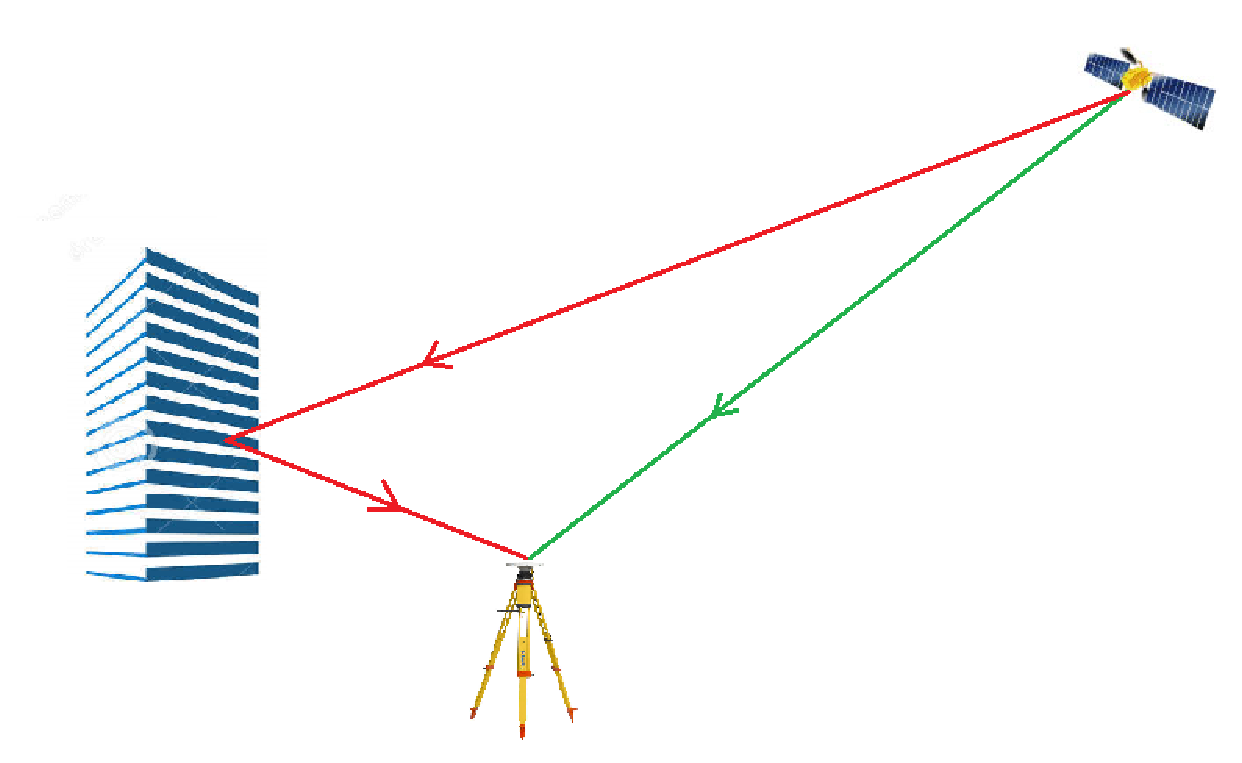
\includegraphics[scale=0.4]{fig/multipath_error.eps} 
	\caption{Multipath error}
	\label{FIG:multipath} 
\end{figure}


\subsubsection{Satellites geometry}

The satellites geometry is one of the main factors that affect the position accuracy. When the satellites are spread, the area of overlap of the signals is small, thus the uncertainty area is relatively small; vice versa, when the satellites are allocated close to each other, the area of overlap of the signals is larger (see figure \ref{FIG:sat_geometry}). The effect of satellites geometry is usually expressed by the DOP\footnote{Dilution Of Precision} index. The different parameters to quantify the goodness of the geometrical configurations are called PDOP\footnote{Position DOP}, HDOP\footnote{Horizontal DOP}, VDOP\footnote{Vertical DOP}, TDOP\footnote{Time DOP} and GDOP\footnote{Geometric DOP}. In particular GDOP index measures the overall accuracy:
%spostare dopo sta parte??

\begin{equation}
	GDOP = \sqrt{{\sigma_{x}}^{2}+{\sigma_{y}}^{2}+{\sigma_{z}}^{2}+{\sigma_{t}}^{2}}
	\label{eq:GDOP}
\end{equation}

where $\sigma$ is the root mean square of the 3D coordinates and time.

\begin{figure}[ht] 
	\centering
	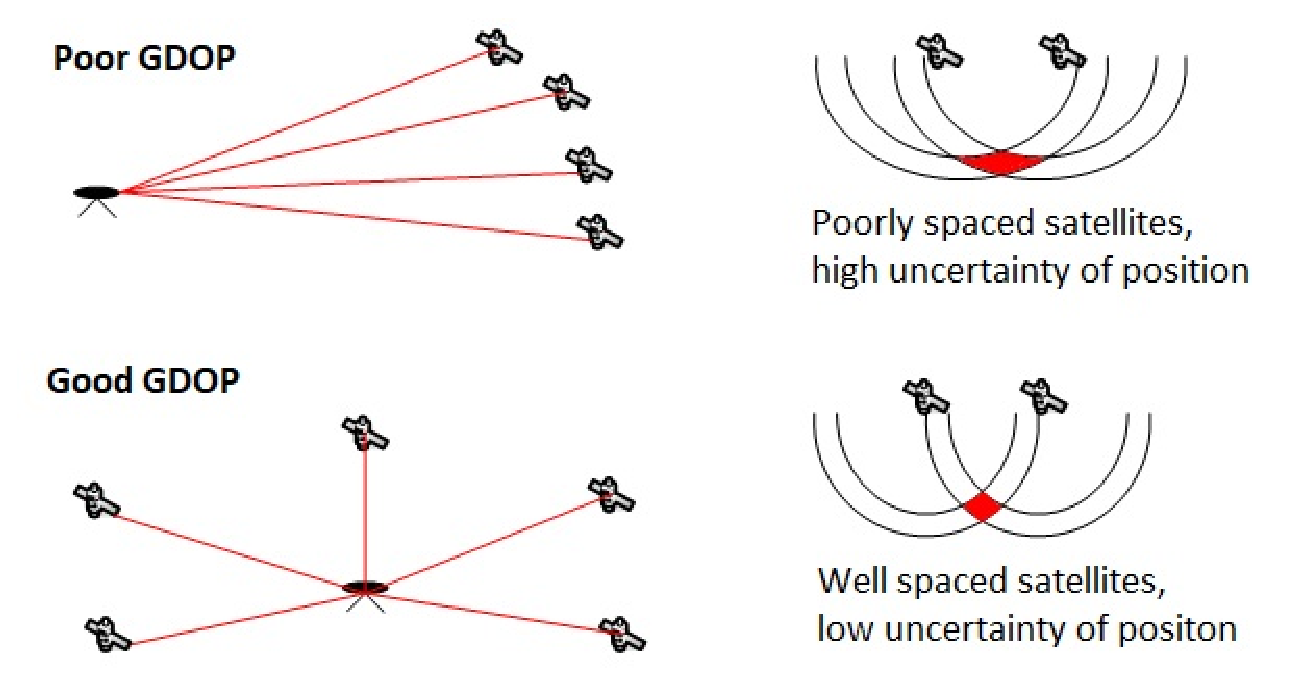
\includegraphics[scale=0.7]{fig/satellites_geometry.eps} 
	\caption{Overlapping signals' areas for spread and close satellites}
	\label{FIG:sat_geometry} 
\end{figure}


\subsection{Relative positioning}

Due to the previously introduced biases, the autonomous point positioning, i.e. \textit{absolute positioning}, can provide accuracy in the order of several meters. To achieve a better positioning precision and to overcome the presence of these errors, several positioning techniques have been developed, typically named \textit{relative positioning}.
Taking into account the main over-mentioned biases, the equation \ref{eq:phase_measure1} can be written as

\begin{equation}
	{\phi_{R}}^{S} = \frac{1}{\lambda}\cdot {\rho_{R}}^{S}(t) + f\cdot \left(\delta^{S}(t) - \delta_{R}(t)\right)+ {N_{R}}^{S}(t) + {I_{R}}^{S}(t) +{T_{R}}^{S}(t) + {E_{R}}^{S}(t)
	\label{eq:sat-receiver_errors}
\end{equation}

where ${I_{R}}^{S}$ is the ionospheric bias, ${T_{R}}^{S} $ is the tropospheric bias and $ {E_{R}}^{S} $ is the ephemerides bias.

Considering two generic receivers A and B, simultaneously observing the same satellite \textit{j}, as shown in figure \ref{FIG:relative_positioning}a, the observation equation \ref{eq:sat-receiver_errors}, could be written as:

%\begin{equation} 
%\begin{matrix} 
%{\phi_{A}}^{j}-f^{j}\cdot\delta^{j}(t) = \frac{1}{\lambda}\cdot {\rho_{A}}^{j}(t) + {N_{A}}^{j}(t) - f\cdot \delta_{A}(t) + {I_{A}}^{j}(t) +{T_{A}}^{j}(t) + {E_{A}}^{i}(t)\\ {\phi_{B}}^{j}-f^{j}\cdot\delta^{j}(t) = \frac{1}{\lambda}\cdot {\rho_{B}}^{j}(t) + {N_{B}}^{j}(t) - f\cdot \delta_{B}(t) + {I_{B}}^{j}(t) +{T_{B}}^{j}(t) + {E_{B}}^{i}(t) \end{matrix} 
%\\
%\label{eq:SingleDifferences1}
%\end{equation}

\begin{equation}\begin{split} 
		{\phi_{A}}^{j}-f^{j}\cdot\delta^{j}(t) & = \frac{1}{\lambda}\cdot {\rho_{A}}^{j}(t) + {N_{A}}^{j}(t) - f\cdot \delta_{A}(t) + {I_{A}}^{j}(t) +{T_{A}}^{j}(t) + {E_{A}}^{i}(t)\\ {\phi_{B}}^{j}-f^{j}\cdot\delta^{j}(t) & = \frac{1}{\lambda}\cdot {\rho_{B}}^{j}(t) + {N_{B}}^{j}(t) - f\cdot \delta_{B}(t) + {I_{B}}^{j}(t) +{T_{B}}^{j}(t) + {E_{B}}^{i}(t) 
		\label{eq:SingleDifferences1}
	\end{split}
\end{equation}

The difference between the two equations in \ref{eq:SingleDifferences1} is

\begin{equation}\begin{split}
		{\phi_{B}}^{j}-{\phi_{A}}^{j} = \frac{1}{\lambda}\cdot \left({\rho_{B}}^{j}(t)-{\rho_{A}}^{j}(t)\right)+ & {N_{B}}^{j}(t)-{N_{A}}^{j}(t)- f^{j}\cdot \left(\delta_{B}(t)-\delta_{A}(t)\right) + \\ {I_{B}}^{j}(t)- {I_{A}}^{j}(t) +{T_{B}}^{j}(t) & - {T_{A}}^{j}(t) + {E_{B}}^{j}(t)-{E_{A}}^{j}(t)
		\label{eq:eq:SingleDifferences1}
	\end{split}
\end{equation}
% la & nelle due righe della equazione serve per dirgli come incolonnarle (le due & corrisponderanno)

This process is called \textit{single differences} (SD). It is important to note that the single differences lead to the elimination of the terms $f^{j}\cdot\delta{j}(t)$ , which are related to the non-synchronization of the satellite’s clock and are common to the two equations in the hypothesis that the two receivers are observing the same satellite $j$.
While the term depending on the satellite clock bias is eliminated by means of single differences, equation \ref{eq:SingleDifferences1} is still sensitive to both receivers clock errors ($\delta_{A}$ and $\delta_{B}$ are still present in the equation).
Introducing the following notations:

\begin{equation} 
	\begin{matrix} 
		{\phi_{AB}}^{j}={\phi_{B}}^{j}-{\phi_{A}}^{j}\\ {\rho_{AB}}^{j}={\rho_{B}}^{j}-{\rho_{A}}^{j}\\{N_{AB}}^{j}={N_{B}}^{j}-{N_{A}}^{j}\\{\delta_{AB}}^{j}={\delta_{B}}^{j}-{\delta_{A}}^{j}\end{matrix}
	\\
	\label{eq:notation1}
\end{equation}

Equation \ref{eq:SingleDifferences1} turns into:

\begin{equation}
	{\phi_{AB}}^{j}(t)=\frac{1}{\lambda}\cdot {\rho_{AB}}^{j}(t)+{N_{AB}}^{j}(t)-f^{j}\cdot{\delta_{AB}}^{j}(t)+\Delta {I_{AB}}^{j}(t)+\Delta {T_{AB}}^{j}(t)+\Delta {E_{AB}}^{j}(t)
	\label{eq:double_diff0}
\end{equation}

Considering two generic receivers A and B, simultaneously observing the same two satellites $i $ and $j$, as reported in figure \ref{FIG:relative_positioning}b, it is possible to write two single differences equations, one for each satellite:

\begin{equation} 
	\begin{split} 
		{\phi_{AB}}^{i}(t)&=\frac{1}{\lambda}\cdot {\rho_{AB}}^{i}(t)+{N_{AB}}^{i}(t)-f^{i}\cdot{\delta_{AB}}^{i}(t)+\Delta {I_{AB}}^{i}(t)+\Delta {T_{AB}}^{i}(t)+\Delta {E_{AB}}^{i}(t)\\ {\phi_{AB}}^{j}(t)&=\frac{1}{\lambda}\cdot {\rho_{AB}}^{j}(t)+{N_{AB}}^{j}(t)-f^{j}\cdot{\delta_{AB}}^{j}(t)+\Delta {I_{AB}}^{j}(t)+\Delta {T_{AB}}^{j}(t)+\Delta {E_{AB}}^{j}(t)  
		\label{eq:double_diff1}
	\end{split}
\end{equation}

Assuming that the two signal frequencies are equal, the difference between the two equations in \ref{eq:double_diff1} is

\begin{equation} 
	\begin{split}
		{\phi_{AB}}^{j}(t)-{\phi_{AB}}^{i}(t) & = \frac{1}{\lambda}\cdot \left({\rho_{AB}}^{j}(t)-{\rho_{AB}}^{i}(t)\right)+{N_{AB}}^{j}(t)- {N_{AB}}^{i}(t) \\ + \nabla\Delta & {I_{AB}}^{ij}(t)  + \nabla \Delta {T_{AB}}^{ij}(t)+\nabla \Delta {E_{AB}}^{ij}(t)
		\label{eq:double_diff2}
	\end{split}
\end{equation}

The symbols $\nabla \Delta$ indicate the double differences operated on the ionospheric, tropospheric and ephemerides biases. This process is called \textit{double differences} (DD). It is important to note that the double differences lead to the elimination of the terms $f^{j}\cdot {\delta_{AB}}^{j}(t)$, which are related to the receivers’ clock bias and are common to the two equations in the hypothesis that the two signal frequencies are the same.

Introducing the notations:
\begin{equation} 
	\begin{matrix} 
		{\phi_{AB}}^{ij}={\phi_{AB}}^{j}-{\phi_{AB}}^{i}\\ {\rho_{AB}}^{ij}={\rho_{AB}}^{j}-{\rho_{AB}}^{i}\\{N_{AB}}^{ij}={N_{AB}}^{j}-{N_{AB}}^{i}\end{matrix}
	\\
	\label{eq:notation2}
\end{equation}

Equation \ref{eq:double_diff2} turns into

\begin{equation}
	{\phi_{AB}}^{ij}(t)=\frac{1}{\lambda}\cdot {\rho_{AB}}^{ij}(t)+{N_{AB}}^{ij}(t)+ \nabla\Delta{I_{AB}}^{ij}(t)  + \nabla \Delta {T_{AB}}^{ij}(t)+\nabla \Delta {E_{AB}}^{ij}(t)
	\label{eq:triple_diff0}
\end{equation}

To remove the time independent ambiguities, two double differences referring to two different epochs could be used, obtaining the \textit{triple differences} (see figure \ref{FIG:relative_positioning}c). Considering two epochs $t_{1}$ and $t_{2}$, it is possible to write two double differences equations, one for each epoch

\begin{equation} 
	\begin{split} 
		{\phi_{AB}}^{ij}(t_{1})&=\frac{1}{\lambda}\cdot {\rho_{AB}}^{ij}(t_{1})+{N_{AB}}^{ij}(t_{1})+\nabla\Delta {I_{AB}}^{ij}(t_{1})+\nabla\Delta{T_{AB}}^{ij}(t_{1})+\nabla\Delta{E_{AB}}^{ij}(t_{1})\\ {\phi_{AB}}^{ij}(t_{2})&=\frac{1}{\lambda}\cdot {\rho_{AB}}^{ij}(t_{2})+{N_{AB}}^{ij}(t_{2})+\nabla\Delta {I_{AB}}^{ij}(t_{2})+\nabla\Delta{T_{AB}}^{ij}(t_{2})+\nabla\Delta{E_{AB}}^{ij}(t_{2})
		\label{eq:triple_diff1}
	\end{split}
\end{equation}

For baselines not exceeding 10-15 km, it is always possible to consider the space correlated ionospheric, tropospheric and ephemerides residuals equal to zero, assuming that the biases are equivalent. The difference between the two equations in \ref{eq:triple_diff2} is

\begin{equation} 
	{\phi_{AB}}^{ij}(t_{2})-{\phi_{AB}}^{ij}(t_{1})=\frac{1}{\lambda}\cdot \left({\rho_{AB}}^{ij}(t_{2})-{\rho_{AB}}^{ij}(t_{1})\right)
	\label{eq:triple_diff2}
\end{equation}

It is important to note that the triple differences lead to the elimination of the terms ${N_{AB}}^{ij}$, which is related to the unknown phase ambiguities. The triple differences is often considered a pre-processing technique to obtain good quality approximate positions for the double differences solution, thanks to the linear combination, which let to remove the ambiguity.

\begin{figure}[ht] 
	\centering
	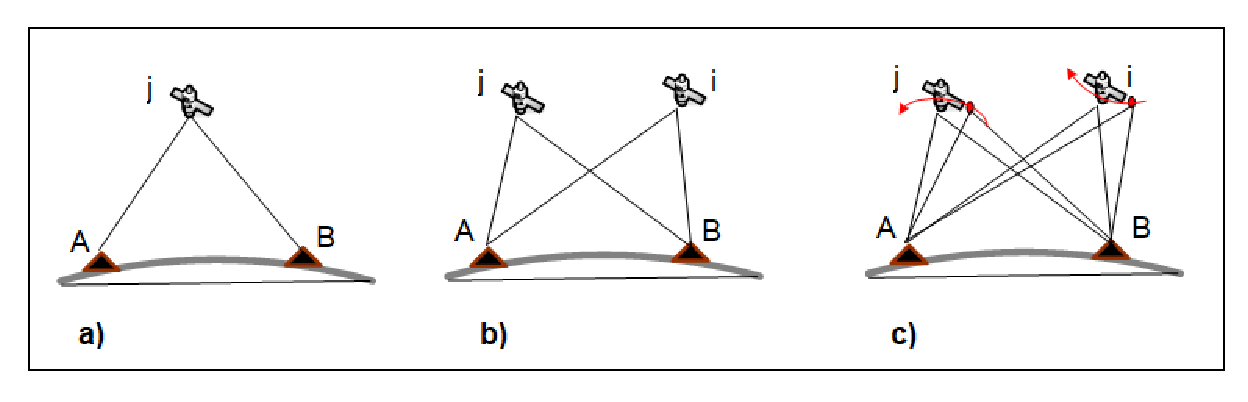
\includegraphics[scale=0.8]{fig/relative_positioning.eps} 
	\caption{Relative positioning assets}
	\label{FIG:relative_positioning} 
\end{figure}

\subsection{RTK positioning}

In general, the determination of the absolute position is less accurate than the relative positioning
between two stations. This is due to the high correlation among the acting errors. To minimize the impact of errors decorrelated with distance, the coordinates
are estimated with respect to a known reference station.
With origin dating back to the mid-1990s, Real Time Kinematics (RTK) is a differential GNSS technique which provides high positioning performance in the vicinity of a base station. The technique is based on the use of carrier measurements and the transmission of corrections from the base station, whose location is well known, to the rover, so that the main errors that drive the stand-alone positioning cancel out. A RTK base station covers a service area spreading about 10 or 20 kilometres, and a real time communication channel is needed connecting base and rover. RTK, which achieves performances in the range of a few centimetres, is a technique commonly used in surveying applications.

From an architectural point of view, RTK consists of a base station, one or several rover users, and a communication channel with which the base broadcasts information to the users in real time.
The technique is based on the following high-level principles:

\begin{itemize}
    \item In the neighbourhood of a clean-sky location, the main errors in the GNSS signal processing are constant, and hence they cancel out when differential processing is used. This includes the error in the satellite clock bias, the satellite orbital error, the ionospheric delay and the tropospheric delay. The main errors left without correction are multipath, interference and receiver thermal noise. Of the errors listed above, the only one which is truly constant with respect to the user location is the satellite clock bias; the rest will show a given dependency with the location as the rover moves away from the base station, being the tropospheric error the first to be fully de-correlated in a few kilometres from the base.
    \item The noise of carrier measurements is much smaller than the one of the pseudo-code measurements. The typical error of code pseudorange measurements is around 1 m, to compare with 5 mm for carrier phase measurements. However, the processing of carrier measurements is subject to the so-called carrier phase ambiguity, an unknown integer number of times the carrier wave length, that needs to be fixed in order to rebuild full range measurements from carrier ones.
    \item The phase ambiguities can be fixed using differential measurements between two reference stations. There are different techniques available to fix them, some based on single frequency measurements with long convergence times, other taking benefit of dual frequency observables with shorter convergence. In general, the techniques either depend on a high precision knowledge of the ionosphere, or assume that the two stations are close enough so that the ionospheric differential delay is negligible when compared with the wave-length of the carriers, around 20 cm. The latter is the approached followed in RTK, limiting the service area to 10 or 20 km; the former is used in WARTK (Wide Area RTK) to cover big service areas with base stations separated around hundreds of kilometres away. The RTK approach needs continuity in the tracked measurements to avoid re-initialization of the phase-ambiguity filters; this is a severe limitation in urban environments due to the big number of obstructions.
\end{itemize}

The base station broadcasts its well-known location together with the code and carrier measurements at frequencies L1 and L2 for all in-view satellites. With this information, the rover equipment is able to fix the phase ambiguities and determine its location relative to the base with high precision. By adding up the location of the base, the rover is positioned in a global coordinate framework.
The RTK technique can be used for distances of up to 10 or 20 kilometres, yielding accuracies of a few centimetres in the rover position, to be compared with 1 m that is achieved with code-based differential GPS. Because of its high precision in controlled environments, RTK is extensively used in surveying applications.
As stated in the previous section, one of the main problems in the RTK technique is fixing the phase ambiguities. The RTK Algorithm is based on double differenced observables that can eliminate selective availability effects as well as other biases (equation \ref{eq:double_diff2}). In this model receiver and satellite clock offsets and hardware biases cancel out. The single difference ambiguities difference $N_{AB}^{j}(t)-N_{AB}^{i}(t)$ is commonly parameterized as a new ambiguity parameter $N_{AB}^{ij}(t)$. The advantage of double differencing is that the new ambiguity parameter $N_{AB}^{ij}(t)$ is an integer because the non-integer terms in the GPS carrier phase observation, due to clock and hardware delays in the transmitter and receiver, are eliminated.
Although it would be possible to estimate the double difference ambiguity using a float approach instead of an integer one, this would lead to dm-level accuracy instead of cm-level. Hence, standard RTK fixes the ambiguities to integer.

Concerning the ambiguity fixing procedure, normally this is done in three steps \cite{Eissfeller:2002}:
\begin{itemize}
\item The ambiguities are first fixed to float numbers using standard least-square techniques.
\item The set of integer ambiguities is set to the one that optimizes the residuals in the surroundings of the float solution.
\item The carrier measurements are corrected with the integer ambiguities, and they are used to obtain the relative position of the rover to the base station.
\end{itemize}

Of these three steps, the second one is quite complex, because the float ambiguity covariance ellipsoid in the measurement space is extremely elongated. As a consequence, the brute-force search process is inefficient, normally beyond the computational capabilities of the rover equipment. Several techniques have been developed to deal with this problem \cite{Laurichesse:2006, Ge:2008, Collins:2008, Teunissen_ar1995, chang2005}.







\subsection{Network-RTK positioning}

One of the major issues related to RTK applications is that the influence of some errors, like
orbit, ionosphere and troposphere, grows with the distance from the reference station. Furthermore,
the impact of the atmospheric error sources depends on solar activity and weather
conditions, which makes the definition of a maximum favorable distance complicated. In order
to overcome this distance-dependent effect, the Network RTK (NRTK) technique has been
developed. The CORS (Continuosly Operating Systems) availability allows the estimate of the state space for the area covered by
the network of reference stations. As a consequence, corrections for a user within the area covered
by the network can be generated and transmitted. Commonly used procedures for NRTK
are the concept of area correction parameters (FKP from the German word Flaechen Korrektur
Parameter), Master Auxiliary Concept (MAC), and Virtual Reference Station (VRS). 
The FKP approach represents additional corrections for the distance-dependent errors by
utilizing a polynomial parametrization to describe the influence of any rover position in a certain
area. These corrections are transmitted in addition to the range corrections of the reference
station considered.
The MAC approach consists in the transmission of observation data of a master station
and correction differences between master and auxiliary stations. The rover can re-construct
the observation data of the auxiliary stations (except a common clock term) and decide how
to use master and auxiliary data for its location.
The VRS approach needs a two-way communication link between rover and network. The
rover communicates their approximate location to the network, which interpolates the observations of all the network station to create and send to the rover a Virtual Reference Station in its proximity. 

%\chapter[State of art]{\begin {Huge}\textit{\bf{State of art}} \end{Huge}}

\chapter[GNSS Raw Measurements and RTKLIB]{\centering \begin{normalsize} \begin{Huge}
		GNSS Raw Measurements and RTKLIB
\end{Huge} \end{normalsize}}
\label{ch:SoA}
%GNSS positioning 
%from Android devices  and 
%This chapter explains the basics of GNSS positioning from Android devices. After highlighting the main research in this area, the Android API that allows access to GNSS raw data in smartphones is explained in detail. The various quantities that can be accessed are then explained and how they can be used to reconstruct classical GNSS observables, i.e. pseudorange, carrier phase, doppler and Signal to Noise Ratio which is an indicator of the quality of the incoming signal. In the latter part of the chapter the GNSS processing software RTKLIB is described. (LB: Non mi convince molto come intro)      
%
\section{GNSS Positioning in Android}
Starting in 2016, with the Android Nougat 7.0 Operating System (OS) development, Google has permitted direct access to the GNSS chipset raw measurements mounted on some Android-based smartphones. The possibility to exploit smartphone GNSS integrated chipset started a new research field aimed at exploiting them in new low-cost applications for satellite-based positioning. 
Even before Google started providing open access to  raw data, the feasibility to perform GNSS positioning using low-cost receivers and smartphone antennas was investigated. In \cite{Pesyna2014} authors showed that centimetric accuracy could be achieved by using a smartphone quality GNSS antenna in relative positioning mode. They also demonstrated that the smartphone GNSS observations are highly affected by the multipath error. In fact, as explained in \cite{Humphreys:2016} the most critical issue is related to the employed GNSS  
 antenna. The smartphone antenna uses linear polarization with non homogeneous gain and high levels of local multipath which render the goal of achieving centimetric accuracy  significantly challenging. Many other researches have been conducted exploring the possibility of managing pseudo-range and carrier phase measurements from the GNSS chipset installed on Android OS smartphones and tablets. 
In a sense, Android OS has changed the concept of precise positioning with portable devices. In this setting different scenarios have been investigated, ranging from urban \cite{Masiero2014, wang2015, wang2016a, wang2016b, adjrad2018} applications  to pedestrian positioning  \cite{Fissore2018, presti2017}, always facing problems related to difficulties in the correct use of the Android Application Programming Interface (API) and of the corresponding filtered measurements provided by the GNSS chipset.

Thanks to the release of a white paper  of the European GNSS Agency \cite{GSA_wp:2016}, in which detailed guidelines on how to reconstruct GNSS measurements using the Android API are given, many authors started to analyze the quality of the raw measurements retrieved from smartphones. The main detected issues in most of the considered experiments were due to the duty cycle mechanism and to low values of the C/N\textsubscript{0} \cite{gogoi2019,Liu:2019} parameter.

In \cite{banville2016} authors conducted an investigation on the quality of the real raw GNSS observations from the smartphones with the purpose of high precision positioning. They analyzed the data collected by a Samsung Galaxy S7 smartphone equipped with the Broadcom 4774 GNSS chip which is able to log raw multi-GNSS (GPS, GLONASS, BDS, Galileo, and QZSS) observations on the L1 frequency. However, in their work, the authors only employed the GPS observations. Since the true position of the smartphone is unknown, they estimated the positioning errors for all components with respect to the mean values of each component. The results indicated that the pseudorange
observations are noisy and only capable of providing meter-level accuracy. They also mentioned that the carrier-phase observations from the smartphones can potentially provide an opportunity to achieve decimeter level or better positioning accuracy. However, to obtain high-accuracy positioning, some important issues such as the quality of the smartphone antenna and the GNSS
duty cycling, a battery saving mode for the GNSS chip causing discontinuities in carrier-phase observations, must be taken into account.
In \cite{Lachapelle2018}, instead, the authors compared the performance of a hand-held GNSS Garmin GPSMap 66 unit with a Huawei P10 smartphone under different conditions including on a rooftop of a building, an urban canyon, indoors and in a car. The results indicated a relatively better performance of the GPSMap 66 with respect to the Huawei P10 which is due to the lower gain advantage of the GPSMap 66 over the P10. It was also shown that the use of an external geodetic antenna can significantly improve data quality and positioning accuracy.
The quality of the raw smartphone observations was also investigated in \cite{Zhang:2018} and the authors draw the same conclusions as the other researchers about the relatively low quality of the smartphone GNSS observations. They also showed that C/N\textsubscript{0} value of GNSS raw observations of the smartphones is 10 dB-Hz lower than the C/N\textsubscript{0} values obtained from a geodetic-quality antenna and receiver. They then combined the pseudorange, carrier-phase and Doppler observations by a time-difference filter positioning algorithm. In this method, they used the Doppler observations to obtain the velocities and then combined them with the single point positioning solutions to achieve the sub-meter level positioning accuracy.
GNSS raw measurement from smartphone were also elaborated using different post-processing techniques. In \cite{Gill2018} authors assessed the accuracy of GPS-only single-frequency PPP with a Nexus 9 smartphone by employing the Global Ionospheric Maps (GIM) to account for the ionospheric delay. The results indicated the RMS of 37 cm and 51 cm for the horizontal and vertical components, respectively, using the cellphone. 
In \cite{realini2017}, the authors demonstrated that it was possible to reach  decimetric  accuracy in terms of positioning performances following the post-processing approach, via a double difference of raw smartphone observations. Meanwhile, the authors of \cite{Dabove2019b} first focused their attention on single-base RTK positioning and then demonstrated the possibility
of obtaining a centimeter-level accuracy through the use of NRTK corrections \cite{Dabove2019b}.
These results are supported by the authors in \cite{pirazzi2017}, who, employing a variometric approach, show decimeter accuracy in static condition and sub-meter when used in an urban vehicle scenario.

Another milestone has been set by Broadcom, announcing on September 21, 2017, the world’s first mass-market, dual-frequency GNSS receiver device, the BCM47755. In May 2018, the Xiaomi Mi8 became the first smartphone in the world, employing a dual-frequency
GNSS receiver L1/E1 – L5/E5a. This led to the next series of studies in the investigation of smartphone-based positioning. 
The NSL’s FLAMINGO (Nottingham Scientific Limited’s fulfilling enhanced location accuracy in the mass-market through Initial Galileo Services) team investigated the PPP and RTK performance of the dual-frequency Xiaomi Mi8 smartphone \cite{Fortunato2019,Roberts2018}. The results confirmed that the carrier-phase observations from the Xiaomi Mi8 were not affected by the duty cycling and employing the L5/E5a observations could improve the positioning accuracy.
Thanks to the double frequency introduced in \cite{Robustelli:2019}, the multipath performance of the Xiaomi Mi8 device were investigated for both E1/L1 E5a/L5 signals using proper linear combination. The results obtained were quite promising, but they seem to indicate again multipath as  one of the main problems for smartphone positioning. Multipath effect on Android devices were studied also in \cite{hakansson:2019} where the author performed a positioning with the Nexus 9 tablet using a particular Eccosorb for multipath mitigation. The results show that precise positioning with uncertainties lower than one meter was possible.
Authors in \cite{Wu2019} also employed the dual-frequency GPS (L1/L5) and Galileo (E1/E5a) observations from a Xiaomi Mi8 smartphone. They have analyzed the positioning performance of the dual-frequency PPP algorithm in both static and kinematic modes. Their numerical results showed that the RMS of the position errors (after convergence to 1 m) was 21.8 cm, 4.1 cm, and 11.0 cm for the East, North, and Up components, respectively, in static mode. However, in kinematic mode, the positioning performance of the PPP algorithm employing the iono-free combination was at the meter-level.
In \cite{Psychas2019} authors evaluated the performance of code-only-based SPP and PPP using the raw GNSS dual-frequency measurements of a Xiaomi Mi8 smartphone with a focus on GPS and Galileo only systems within a 14 hours time span dataset. They provided static positioning solutions in different cases for example single-frequency uncombined (GPS-only and Galileo-
only), combined (GPS + Galileo) models, dual frequency uncombined and combined models in
both real-time and post-processing modes. They then assessed the performance of these solutions in terms of their repeatability and accuracy with respect to the true position of the pillar where the smartphone was placed. It was shown that the dual-frequency GPS + Galileo
SPP solution had a better performance compared with the single-frequency uncombined SPP. The PPP
solutions were also converged to the sub-meter level accuracy in all different cases. However, based on the results, the combined GPS + Galileo solution resulted in reducing the convergence time to the sub-meter level horizontally accuracy.

Accessing GNSS raw data from smartphones opens the way to various applications not only related to positioning. Properly processed, such data can be used to monitor the troposphere by estimating the ZTD (Zenith Total Delay). In \cite{benvenuto:2021} authors shows encouraging results in the ZTD estimation by smartphone\footnote{Paper published on 13\textsuperscript{th} November 2021: \url{https://www.mdpi.com/2072-4292/13/22/4567}}.

Besides Xiaomi Mi8 and Nexus 9, there are many other devices providing low level access to GNSS raw measurements. 
Nowadays raw GNSS measurements support is mandatory on devices that run Android 10 (API level 29) or higher, but unfortunately the support for some of the raw GNSS measurement fields is optional and can vary depending on the used GNSS chipset. Important fields that some devices may not have, are the following:
\begin{itemize}
\item Pseudorange and pseudorange rate;
\item Navigation message;
\item Accumulated Delta Range (ADR) or carrier phase;
\item Automatic Gain Controller (AGC) value.
\end{itemize}
Furthermore, not all the smartphone present on the market support double frequency or multi-constellation data. A non-exhaustive list of Android-powered devices with their support level of raw GNSS measurements can be found in the Android developer web page\footnote{\url{https://developer.android.com/guide/topics/sensors/gnss}}. Some more information can be found in the literature as well. For instance, as shown in \cite{darugna2021}, there are 41 smartphone models on the market, from 10 manufacturers,  offering dual-frequency capability. The number is increasing continuously. For example, one of the recent launches by a major manufacturer was the Galaxy Note10 and Galaxy Note10+ from Samsung Electronics, which hit the market in the second half of 2019. These smartphones are equipped with the BCM47755, like the HuaweiMate20X (Mate20X). Huawei also developed its chipset, embedded in, for example, the Huawei P30. Moreover, Qualcomm developed another chipset that is employed, e.g., in the Google Pixel 4 and Pixel 4XL. 
More detailed information about dual-frequency smartphone capability can be found at the UseGalileo web page provided by GSA\footnote{\url{https://www.usegalileo.eu/EN/inner.html#data=smartphone}}.
%\marginpar{Mettere una sitografia?}
\section{API description}

One of the sensors embedded in smartphones is GNSS receiver. This sensor is used by all the applications that need to retrieve the user position. In general, the main idea of Android devices is to obtain
a good enough position for the common users’ purposes, as for example finding the fastest path to reach points of interest using Google Maps.

The Android system provides a series of functions called
Application Programming Interface (API) allowing users
to access the system's functionalities. Each version of the
Android system has different types of APIs.
Prior to 2016, the API to interact with the GNSS chipset embedded in the smartphone was the \textit{android.gms.location}. 

\begin{figure}[H] 
	\centering
	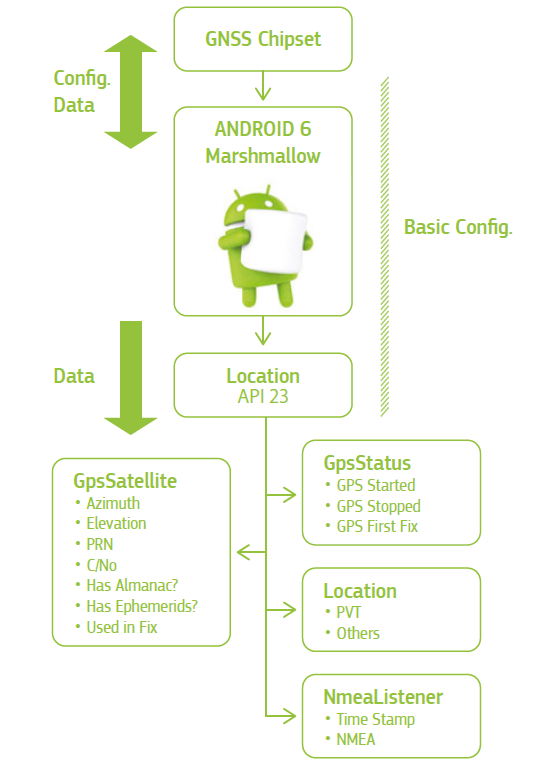
\includegraphics[scale=0.75]{fig/android6API.png} 
	\caption{location API in Android 6}
	\label{FIG:locapiand6} 
\end{figure}

As shown in figure \ref{FIG:locapiand6}, only some basic information computed by the GNSS chipsets were available to the
users. In particular, it was possible to access some GPS satellites information (e.g., C/N\textsubscript{0}, azimuth, and elevation) as well as the basic NMEA (National
Marine Electronics Association) sentences which include
the PVT (Position Velocity and Time) solution. The raw GNSS observations (e.g., pseudorange
and carrier-phase measurements) could not be accessed.  

Starting from the Nougat version (Version 7), Android introduces the new Location API namely \textit{android.location} (figure \ref{FIG:locapiand7}) which gives access to the GNSS raw measurements. However, the new API
implemented on Android 7 does not provide the GNSS measurements directly (e.g., pseudorange, carrier phase and Doppler observations) but the GNSS measurements must be extracted from the raw data logged.
The next paragraphs explain how to obtain GNSS time, pseudoranges,
carrier-phase and Doppler measurements from data contained in \textit{android.location} API. 

\begin{figure}[H] 
	\centering
	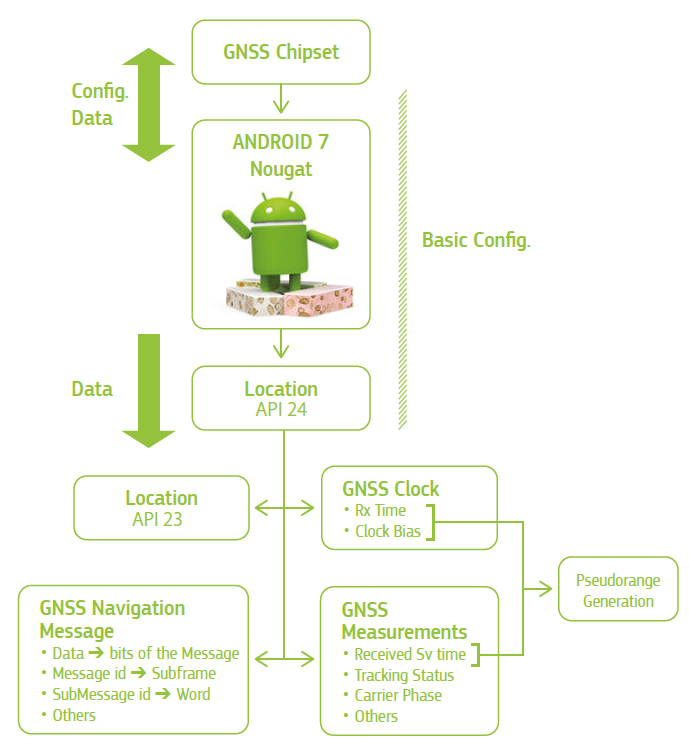
\includegraphics[scale=0.75]{fig/android7API.png} 
	\caption{location API in Android 7}
	\label{FIG:locapiand7} 
\end{figure}

In order to process GNSS measurements from smartphones using common GNSS processing software, as for example RTKLIB \cite{takasu:2009}, the GNSS observation should be derived and written in a standarized format, e.g. RINEX (Receiver INdipendent EXchange format)\footnote{\url{http://acc.igs.org/misc/rinex304.pdf}}. 
Starting from Android 7, GNSS raw observation can be reconstructed by using the informations contained in \textit{Android location API} from level 24 and above see figure \ref{FIG:locapiand7}. The strategy to reconstruct GNSS raw observation is illustrated in \cite{GSA_wp:2016} and hereafter summarized. All the needed information can be retrieved from three classes of \textit{Android location API}:
\clearpage
\begin{itemize}
	{\item GNSS Clock, that contains:}
	\begin{itemize}
		{\item Receiver Time;}
		{\item Clock bias.}
	\end{itemize}
	{\item GNSS Measurement, that contains:}
	\begin{itemize}
		{\item Received Satellite Time;}
		{\item Code;}
		{\item Carrier Phase.}
	\end{itemize}	
	{\item GNSS Navigation Message, that contains:}
	\begin{itemize}
		{\item Navigation Message bits;}
		{\item Navigation Message status.}
	\end{itemize}	
	
\end{itemize}

Table \ref{tab:api_fields} summarizes the most important fields used to reconstruct raw measurements, while table \ref{tab:api_constants} shows the main constants that should be taken into account for the measurement generation, as latter explained.

\begin{table}[H]
	\centering
	\begin{tabular}{|c|c| p{5cm}|}
	\hline
	\textbf{Class} & \textbf{Field} & \textbf{Description}\\
    \hline
	GNSSclock & TimeNanos & GNSS receiver’s internal hardware clock value in nanoseconds\\  
    \hline
	GNSSclock & BiasNanos & Clock’s sub-nanosecond bias\\  
    \hline
	GNSSclock & FullBiasNanos & Difference between TimeNanos inside the	GPS receiver and the true GPS time since 6\textsubscript{th} January 1980\\  
    \hline
	GNSSMeasurement & TimeOffestNanos & Time offset at which the measurement was taken in nanoseconds.\\
    \hline
	GNSSMeasurement & ConstellationType & Constellation type\\  
    \hline
    GNSSMeasurement & Svid & Satellite ID\\  
    \hline
    GNSSMeasurement & State & Per-satellite sync state.	It represents the current	sync state for the associated satellite\\  
    \hline
	GNSSMeasurement & ReceivedTimeNanos & Received GNSS satellite time, at the measurement	time, in nanoseconds\\  
    \hline
	GNSSMeasurement & AccumulatedDeltaRangeMeters & Accumulated delta range since the last channel reset, in meters\\  
    \hline
    GNSSMeasurement & AccumulatedDeltaRangeState & Accumulated Delta Range state\\  \hline
    GNSSMeasurement & CarrierFrequencyHz & Carrier frequency at which codes and messages are modulated\\  
    \hline
    GNSSMeasurement & PseudorangeRatemetersperSecond & Gets the Pseudorange rate at the timestamp\\ 
    \hline
	\end{tabular}
	\caption{Android Location API - Clock and Measurements fields.}
	\label{tab:api_fields}
\end{table}

\begin{table}[H]
	\centering
	\begin{tabular}{| c | c| }
		\hline
		\textbf{Constant} & \textbf{Value (Hexadecimal)}\\
		\hline 
		STATE TOW KNOWN & 0x00004000 \\  
		\hline
		STATE GLO TOD KNOWN & 0x00008000 \\
		\hline
		STATE GAL E1C 2ND CODE LOCK & 0x00008000\\     
		\hline	
	\end{tabular}
	\caption{Android Location API - GNSSMeasurements constants.}
	\label{tab:api_constants}
\end{table}

The quantities retrieved by the proposed program are the pseudorange, the carrier phase, the doppler and C/N\textsubscript{0}. In the following sections, different strategies to compute these quantities are illustrated in details. The methods described were implemented, in the ambit of this work, in a modified version of RTKLIB capable of working with GNSS data from Android (see Appendix \ref{appendix:mrtklib_andr}).
\subsection{Pseudorange computation}  
The equation for the pseudorange is:
\begin{equation}
	\rho = c \cdot (t_{A}-t_{E})
	\label{eq:psrange}
\end{equation}
where \textit{c} is the speed of light, \textit{t\textsubscript{A}} the acquisition time and \textit{t\textsubscript{E}} the emission time of the signal. In the case of smartphones,  \textit{t\textsubscript{A}} and  \textit{t\textsubscript{E}} are calculated considering the \textit{GNSS Clock} class (used for receiver-related quantities) and the  \textit{GNSS Measurement} class. 
The receiver time is generated considering the TimeNanos quantity, which is the GNSS receiver’s internal hardware clock provided as an integer number of nanoseconds. The FullBiasNanos quantity, i.e., the difference between the TimeNanos inside the GPS receiver and the true GPS time since the 6\textsuperscript{th} of January 1980 must be subtracted to the TimeNanos in order to get the true GPS time. So the receiver time can be written as:

\begin{equation}
	T_{Rx} = TimeNanos - FullBiasNanos
	\label{eq:Trx_int}
\end{equation}

The API also provides the BiasNanos quantity, i.e. the clock’s sub-nanosecond bias (varying between 0 and 1), which allows getting a more accurate timing. Considering also the BiasNanos, the receiver time becomes:

\begin{equation}
	T_{Rx} = TimeNanos - (FullBiasNanos + BiasNanos)
	\label{eq:Trx_flt}
\end{equation}
Both the GNSS RawMeasurements Task Force \cite{GSA_wp:2016} and Google in its GNSS analysis tool available online suggest considering only the first value of the FullBiasNanos and BiasNanos and keep them constant for all the acquisition. In this work, as suggested in \cite{darugna2021}, FullBiasNanos and BiasNanos are updated every epoch. Indeed, in \cite{darugna2021} the authors observe that, depending on the device firmware, FullBiasNanos values can have significant oscillations, hence they cannot be considered as constant.


The received satellite time, i.e. ReceivedSvTimeNanos, is relative to the beginning of the system week for all constellations except for GLONASS, where it is relative to the beginning of the GLONASS system day. Therefore, depending on the GNSS involved, the condition of
reliability of the received satellite time is satisfied if:

\begin{itemize}
	{\item  GPS, Galileo, and BeiDou: STATE TOW KNOWN constant flag is set}
	{\item  GLONASS: STATE GLO TOD KNOWN constant flag is set}
\end{itemize}

The constant values of STATE TOW KNOWN and STATE GLO TOD KNOWN are reported in table \ref{tab:api_constants}.

These flags provide an insight into the state of the tracking algorithms that must be taken into account to verify the reliability of the measurement. It’s worth mentioning that some devices track the Galileo E1C component, and the tracking status is flagged as the STATE GAL E1C 2ND CODE LOCK (see table \ref{tab:api_constants}). In this case, the ambiguity of the pseudorange is 100ms, another parameter to take into account.

The satellite emission time can be than computed as:

\begin{equation}
	T_{E,TOW} = ReceivedTimeNanos
	\label{eq:Te_tow}
\end{equation}
 
in GPS Time Of theWeek (TOW) for GPS, Beidou and Galileo, and

\begin{equation}
	T_{E,TOW} = ReceivedTimeNanos
	\label{eq:Te_tod}
\end{equation}

in GPS Time Of the Day (TOD) for GLONASS.

Once the receiver and satellite time have been computed, the pseudorange observation can be reconstructed. Receiver and satellite time as computed in eq \ref{eq:Trx_flt} and eq \ref{eq:Te_tow} (or eq \ref{eq:Te_tod}) are expressed in GPS time and GPS TOW/TOD, respectively. To solve this data type inconsistency, two possible options are possible:

\begin{itemize}
	\item to compute the receiver time in GPS TOW;
	\item to compute the satellite time in GPS time.
\end{itemize}

In the first case the receiver time can be computed in the following ways.

For GPS and Galielo:

\begin{equation}
	T_{Rx} = mod(T_{Rx,GT},NanoSecondsWeek)
	\label{eq:Trx_gps_gal_tow}
\end{equation}

For Beidou:

\begin{equation}
	T_{Rx} = mod(T_{Rx,GT},NanoSecondsWeek) + 14\cdot10^{9}
	\label{eq:Trx_beid_tow}
\end{equation}

And for GLONASS:

\begin{equation}
	T_{Rx} = mod(T_{Rx,GT},NanoSecondsDay) + (7200-ls)\cdot10^{9}
	\label{eq:Trx_glo_tow}
\end{equation}

Where \textit{NanoSecondsWeek} is the number of nanoseconds in a week, and \textit{NanoSecondsDay} and \textit{ls} (see eq \ref{eq:Trx_glo_tow}) are the nanoseconds in a day and the leap seconds respectively.

In the latter case, i.e., when computing satellite time in GPS time, the equation for GPS and Galileo becomes:

\begin{equation}
	T_{E} = T_{E,TOW} + nw\cdot NanoSecondsWeek
	\label{eq:Te_gps_gal_gpstime}
\end{equation}

While the equantion for BeiDou is:

\begin{equation}
	T_{E} =  T_{E,TOW} + nw\cdot NanoSecondsWeek +  14\cdot10^{9}
	\label{eq:Te_beidou_gpstime}
\end{equation}

And for GLONASS:

\begin{equation}
	T_{E} =  T_{E,TOD} + NanoSecondsDaySince1980 +  (7200-ls)\cdot10^{9} 
	\label{eq:Te_glo_gpstime}
\end{equation}

Where \textit{nw} (see equations \ref{eq:Te_gps_gal_gpstime} and \ref{eq:Te_beidou_gpstime}) is the number of weeks since 6\textsuperscript{th} January 1980, and \textit{NanoSecondsDaySince1980} is the days since 6\textsuperscript{th} January 1980 in nanoseconds.

Lastly, for each observation, the time offset at which the measurement was taken with regard to the TimeNanos has to be considered: this quantity is given by TimeOffsetNanos. The acquisition time  becomes then:

\begin{equation}
	T_{A} =  T_{Rx} + TimeOffsetNanos
	\label{eq:Ta_android}
\end{equation}

Finally, the pseudorange observation can be computed in meters in the followig way:

\begin{equation}
	\rho = \frac{ c \cdot (T_{Rx}-T_{E})}{10^{9}}
	\label{eq:pseudorange_android}
\end{equation}

\subsection{Carrier Phase observation computation}

Carrier phase measurements are provided directly by API the  as \textit{AccumulatedDeltaRangeMeters} in metres. Often in GNSS standard format the phase measurement are expressed in number of cycles and not in meters. In order to express the phase measurement in cycles, the \textit{AccumulatedDeltaRangeMeters} should be divided by the wavelength.

\begin{equation}
	\phi = \frac{AccumulatedDeltaRangeMeters}{\lambda}
	\label{eq:phase_cycles}
\end{equation}

The $\lambda$ value can be obtained from the API, by dividing the field \textit{CarrierFrequencyHz} by the speed of light.
 
Carrier phase observation are ambiguous, without the time information, meaning the receiver can only count the number of cycles occurring between epochs (as explained in riferimento capitolo1), and, for example if a cycle slip occurs, the receiver loses this count. For this and also other reasons the \textit{AccumulatedDeltaRangeMeters} field is paired with the \textit{AccumulatedDeltaRangeState}. The \textit{AccumulatedDeltaRangeState}, which values are reported in table \ref{tab:adr_state}, it's possibile to check the validity status of the carrier phase observation.

\begin{table}[h]
	\centering

	\begin{tabular}{| c | c| c|}
		\hline
		\textbf{Status} & \textbf{Value} & \textbf{Description)}\\
		\hline 
		ADR STATE CYCLE SLIP & 4 & A cycle slip has been detected.\\
		\hline
		ADR STATE RESET & 2 & A reset has been detected.\\
		\hline
		ADR STATE VALID & 1 & State is valid.\\     
		\hline	
		ADR STATE UNKNOWN & 0 & State is unknown.\\     
		\hline
	\end{tabular}
\caption{Accumulated delta range state valued}
\label{tab:adr_state}
\end{table}

Concerning carrier phase observation on smartphones, it is worth mentioning the potential problems related to duty cycle. The duty cycle is a process where the GNSS chipset of the smartphone works in a discontinuous way, which causes the hardware clock to be active only for a fraction of each second to support low power consumption and, thus, reduce battery consumption. \cite{Linty:2014}. 

\begin{figure}[htb] 
	\centering
	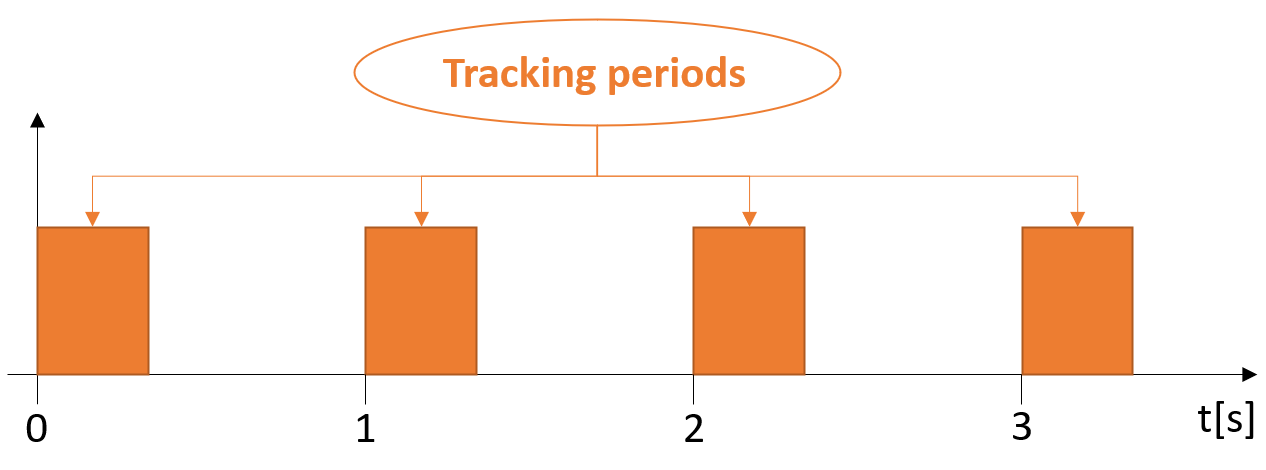
\includegraphics[scale=0.60]{fig/duty_cycle.png} 
	\caption{Duty cycle versus time}
	\label{FIG:duty_cycle} 
\end{figure}
As explained in \cite{GSA_wp:2016}, there are two different implementations of the duty-cycle that depend on the GNSS clock status:
\begin{itemize}
	\item TCXO Hardware clock is not continuous (turning on and off) during the non-tracking periods;
	\item TCXO Hardware clock is continuous during the non-tracking periods.
\end{itemize}
The smartphone has two oscillators: higher precision compensated for temperature variations (TCXO) that is being used for GNSS tracking and an alternative, low-power consumption, crystal oscillator (XO). In the first case, during the short tracking period, when the chipset tracks GNSS data, TCXO is used. 
Out of this period, when a chip shuts down for several hundreds of milliseconds, XO is providing time. In the latter case, when the GNSS chipset is turned off, the TCXO clock keeps running, even though no signal is being tracked. 
Users cannot detect when the receivers are operating in
duty cycle. Without going in further details, which is not the purpose of this work, it should be clear that duty cycle has
an impact on the carrier phase measurements. Indeed, without tracking continuity, several cycle slips may occur between two
consecutive measurements, severely limiting the use of  advance phase techniques such as Real Time Kinematic.

Starting from Android 9, it has been introduced an option to disable the duty cycle. Thanks to this option, it's possible to use GNSS carrier phase observation from smartphone.

\subsection{Doppler computation}
 The Doppler shift that results from satellite movement can be derived from the \textit{PseudorangeRateMetersPerSecond}, provided
 that the pseudorange rate, at the timestamp, is in m/s. In particular it's given by:
 
 \begin{equation}
 	Dopplershift = -\frac{PseudorangeRateMetersPerSecond}{\lambda}  	\label{eq:doppler_and}
 \end{equation}

Where $\lambda$ is the wavelength.

Once the GNSS raw observable are reconstructed they can be processed by common GNSS processing software in order to retrieve the position following the principles illustrated in chapter \ref{ch:gnss}. 


In this thesis work, the software library used for all experiments are based on RTKLIB. This software is widely use from the scientific community for research purposes on GNSS.
It implements different positioning methods and, being open source, it can be easily modified and adapted to specific cases. As latter explained, in the ambit of this work, the RTKLIB software library has been modified in order both to work in real time with data coming from Android smartphones and to implement an algorithm for increasing the positioning robustness. In the following paragraph the RTKLIB software is illustrated in details, with particular attention to the algorithms that i natively implements for GNSS positioning.

\section{RTKLIB for data processing}
RTKLIB \cite{takasu:2009}  is an open source portable program library written in C and C++ which provides a platform for precise GNSS positioning. The current version of the library is distributed under the following BSD 2-clause license and additional exclusive clauses. Previous versions of RTKLIB until ver. 2.4.1 had been distributed under GPLv3 license.
The quite satisfactory performance of the library and  specific characteristics of the licence, which allows free exploitation for commercial applications made RTKLIB, made it very popular and extensively exploited. 
\subsection{Software description}
The library implements fundamental navigation functions and carrier-based relative positioning algorithms both in real time as well as in post processing. In spite of its name, however, it is not limited to RTK relative positioning but implement also many other stand alone and relative positioning techniques, like Single, DGPS/DGNSS, Kinematic, Static, Moving-Baseline, Fixed, PPP-Kinematic, PPP-Static and PPP-Fixed.
RTKLIB is able to estimate integer ambiguity exploiting the LAMBDA method \cite{Teunissen_ar1995} . 
RTKLIB was originally developed under the Windows Operating System, and later it has been ported under UNIX environment which allows to use it in small and compact single-board computer, as for example, the Raspberry integrated into the PID. 
RTKLIB is a GNSS processing software since, in addition to GPS, it supports also GLONASS, GALILEO, QZSS, BeiDou and SBAS.
Moreover it supports many standard formats and protocols for GNSS: 
\begin{itemize}
\item RINEX 2.10, 2.11, 2.12 OBS/NAV/GNAV/HNAV/LNAV/QNAV,
\item RINEX 3.00, 3.01 OBS/NAV,
\item RINEX 3.02 OBS/NAV/CLK,
\item RTCM 2.3, 3.1(with amendment 1-5), 3.2,
\item BINEX,
\item NTRIP 1.0,
\item RTCA/DO-229C,
\item NMEA 0183,
\item SP3-c,
\item ANTEX 1.4,
\item IONEX 1.0, 
\item NGS PCV and EMS 2.0.
\end{itemize}

RTCM (Radio Technical Commission for Maritime Services) standar in particular, is a communication protocol for sending differential corrections to a GNSS receiver from a secondary source. The format does not define the source of the messages and has been used with systems as varied as longwave marine radio, communications satellite broadcasts, and internet distribution. NTRIP (Networked Transport of RTCM via Internet Protocol) instead is an application-level protocol that
supports streaming GNSS data over the Internet. which is meant to be an open non-proprietary protocol.

RTKLIB supports also several GNSS receivers' proprietary messages like NovAtel, OEM4/V/6, OEM3, OEMStar, Hemisphere, u-blox, JAVAD and other. 
It also supports external communication via: Serial port, TCP/IP, NTRIP, local log file (record and playback) and FTP/HTTP (automatic download).
The library include a full set of functions suitable to be exploited both for geodesy or precise navigation application and the processing is configurable to optimize the retrieved solution. 
Among the different function it's worth mentioning: 
\begin{itemize}
\item matrix and vector computation functions,
\item time and string functions,
\item coordinates transformation, 
\item input and output functions,
\item debug trace functions, platform dependent functions, 
\item positioning models, 
\item atmosphere, antenna, earth tides ocean loading models, 
\item geoid models and  datum transformation, 
\item precise ephemeris and satellite clock handling functions, 
\item Google Earth KML converter, 
\item SBAS functions, 
\item integer ambiguity resolution, 
\item standard positioning, real time precise positioning and post-processing positioning, 
\item stream and  RTK server functions, 
\item downloader functions
\end{itemize}
Going into details, RTKLIB provides APIs for real-time positioning, post-processing analysis, and positioning utilities. Table \ref{tab:rtklib_apps} shows the main RTKLIB APPs in their GUI (Graphical User Interface) version and CUI (Command-line User Interface) version. In the ambi of this work the CUI APs are used and in particular RTKRCV for computing the Real-Time Positioning.
\begin{table}[ht]
	\centering
	\begin{tabular}{| c | c| c|}
		\hline
		\textbf{Function} & \textbf{GUI App} & \textbf{CUI App}\\
		\hline 
		App launcher & RTKLAUNCH  & -\\
		\hline
		Real time positioning & RTKNAVI & RTKRCV\\
		\hline
		Communication Server & STRSVR & STR2STR\\     
		\hline	
		Post processing analysis & RTKPOST & RNX2RTKP\\     
		\hline
		RINEX Converter & RTKCONV & CONVBIN\\     
		\hline
		Plot solutions and observation data & RTKPLOT & -\\     
		\hline
		Download GNSS data and products & RTKGET & -\\     
		\hline
	\end{tabular}
\caption{RTKLIB Apps}
\label{tab:rtklib_apps}
\end{table}
\subsection{Software computation strategy}
RTKLIB, as well explained in \cite{takasu:2009}, uses algorithms for differential GNSS positioning. In particular, for carrier-based relative
positioning with a short length baseline between rover \textit{a} and
base-station \textit{b}, the equation \ref{eq:triple_diff0} is used. This equation can be also written as
\begin{equation} 
	\begin{matrix} 
		{\Phi_{ab}}^{ij}={\rho_{ab}}^{ij}+\lambda(B_{ab}^{i}-B_{ab}^{j})+ \textit{d}\Phi_{a}^{S}+\epsilon_{\Phi}\\ 
		{P_{ab}}^{ij}={\rho_{ab}}^{ij}+  \epsilon_{P}
		\end{matrix}
	\\
	\label{eq:ddiff_rtklib}
\end{equation}

where $\rho$ is the geometric range, $\lambda$ is the carrier wave length and $\epsilon$ is the measurement error of 
these observables, $B_{ab}^{i}$ is single-difference of carrier-phase ambiguities in cycle, and $\textit{d}\Phi_{a}^{S}$ is the carrier‐phase correction terms, which can be neglected in the short‐baseline case.
Thanks to the double differencing procedure, equations are free of satellite and receiver clock-biases, and
atmospheric effects, as explained in chapter \ref{ch:gnss}.
After computing these equations, a vector \textbf{\textit{x}} containing the unknown state for RTK-GPS positioning is set:

\begin{equation} 
	\begin{matrix} 
		{\textbf{\textit{x}}}=({\textbf{\textit{r}}_{a}}^{T}+{\textbf{\textit{B}}_{L1}}^{T}+{\textbf{\textit{B}}_{L2}}^{T} + +{\textbf{\textit{B}}_{L5}}^{T})^{T}\\ 
		\textbf{\textit{B}}_{Lj}=({{B}_{Lj}}^{1}, {{B}_{Lj}}^{2},...,{{B}_{Lj}}^{m})^{T}
		\end{matrix}
	\\
	\label{eq:unkstate_rtklib}
\end{equation}
where $\textbf{\textit{r}}_{a}$ is rover antenna position in ECEF frame, and $m$ is the number of satellites used. The measurement vector ${\textbf{\textit{y}}}_{k}$ at the epoch $\textit{t}_{k}$ is
defined with double-differenced carrier-phase and pseudorange
measurements as:

\begin{equation} 
	\begin{matrix} 
		\textbf{y}_{k}= ({\boldsymbol{\Phi}_{L1}}^{T}, {\boldsymbol{\Phi}_{L2}}^{T},{\boldsymbol{\Phi}_{L5}}^{T}, {\textbf{P}_{L1}}^{T},{\textbf{P}_{L2}}^{T}, {\textbf{P}_{L5}}^{T})^{T}\\ 
		\boldsymbol{\Phi}_{Lj}= ({\Phi_{ab,lj}}^{12},{\Phi_{ab,lj}}^{13},...,{\Phi_{ab,lj}}^{1m})^{T}\\
        \textbf{P}_{Lj}= ({P_{ab,lj}}^{12},{P_{ab,lj}}^{13},...,{P_{ab,lj}}^{1m})^{T}\\
		\end{matrix}
	\\
	\label{eq:measvector_rtklib}
\end{equation}

RTKLIB estimates the state vector
\textbf{\textit{x}} and its covariance matrix \textbf{\textit{P}} using a standard EKF Extended Kalman Filter \cite{kalman:1960, grewal2001}. The used equations are:

\begin{equation} 
	\begin{matrix} 
		\hat{\textbf{\textit{x}}_{k}}(+)= \hat{\textbf{\textit{x}}_{k}}(-) + \textbf{\textit{K}}_{k}\cdot \left[ \textbf{\textit{y}}_{k}-\textbf{\textit{h}}\left(\hat{\textbf{\textit{x}}_{k}}(-)\right) \right]\\ 
		\textbf{\textit{P}}_{k}(+)= \left(\textbf{\textit{I}}-\textbf{\textit{K}}_{k} \textbf{\textit{H}}_{k}\left(\hat{\textbf{\textit{x}}_{k}}(-) \right)\right) \left( \textbf{\textit{P}}_{k}(-)\right)\\
		\textbf{\textit{K}}_{k}= \textbf{\textit{P}}_{k}(-)\textbf{\textit{H}} \left( \hat{\textbf{\textit{x}}_{k}}(-) \right) \left( \textbf{\textit{H}} \left( \hat{\textbf{\textit{x}}_{k}}(-) \right) \textbf{\textit{P}}_{k}(-) \textbf{\textit{H}} \left( \hat{\textbf{\textit{x}}_{k}}(-) \right)^{T} + \textbf{\textit{R}}_{k} \right)^{-1}
		\end{matrix}
	\\
	\label{eq:EKF_rtklib}
\end{equation}
Where $\textbf{\textit{h(x)}}$, $\textbf{\textit{H(x)}}$ and \textbf{\textit{R\textsubscript{k}}} are the measurements model vector, the
matrix of partial derivatives and the covariance matrix of
measurement errors, respectively. Considering equations \ref{eq:ddiff_rtklib} they can be written as:
\begin{equation} 
	\begin{matrix} 
		\textbf{\textit{h}}(\hat{\textbf{\textit{x}}})= \left( {\textbf{\textit{h}}_{\Phi,L1}}^{T}, {\textbf{\textit{h}}_{\Phi,L2}}^{T},  {\textbf{\textit{h}}_{\Phi,L5}}^{T}, {\textbf{\textit{h}}_{P,L1}}^{T}, {\textbf{\textit{h}}_{P,L2}}^{T}, {\textbf{\textit{h}}_{P,L5}}^{T}\right)\\
		\textbf{\textit{h}}_{\Phi,Lj} = \begin{bmatrix} 
                {\rho_{ab}}^{12} + \lambda_{Lj} \left( B_{ab,Lj}^{1} - B_{ab,Lj}^{2} \right)  \\
                {\rho_{ab}}^{13} + \lambda_{Lj} \left( B_{ab,Lj}^{1} - B_{ab,Lj}^{3} \right)  \\
                \vdots\\
               {\rho_{ab}}^{1m} + \lambda_{Lj} \left( B_{ab,Lj}^{1} - B_{ab,Lj}^{m} \right)  \\ \\
                \end{bmatrix}, & \textbf{\textit{h}}_{P,Lj} = \begin{bmatrix} 
                {\rho_{ab}}^{12}  \\
                {\rho_{ab}}^{13}  \\
                \vdots\\
               {\rho_{ab}}^{1m}  \\
                \end{bmatrix} 
        
		\end{matrix} \\
	\label{eq:EKF_rtklib_h}
\end{equation}

\begin{equation}
	\textbf{\textit{H}}(\hat{\textbf{\textit{x}}}) = \frac{\partial \textbf{\textit{h}}(\hat{\textbf{\textit{x}}})}{\partial \textbf{x}} \bigg|_{x=\hat{x}} = \begin{bmatrix}
	    \textbf{\textit{-DE}} & 0 & \lambda_{L1}\textbf{\textit{D}} &0&0\\
	    \textbf{\textit{-DE}} & 0 & 0 &\lambda_{L2}\textbf{\textit{D}}&0\\
	    \textbf{\textit{-DE}} & 0 & 0 &0&\lambda_{L5}\textbf{\textit{D}}\\
	    \textbf{\textit{-DE}} & 0 & 0 &0&0\\
	    \textbf{\textit{-DE}} & 0 & 0 &0&0\\
	    \textbf{\textit{-DE}} & 0 & 0 &0&0\\
	\end{bmatrix}
	\label{eq:EKF_rtklib_H}
\end{equation}

\begin{equation}
\begin{matrix}
\textbf{\textit{R}}_{k} = \begin{bmatrix}
\textbf{\textit{D}}\textbf{\textit{R}}_{\Phi,L1}{\textbf{\textit{D}}}^{T} &&&&&\\
&\textbf{\textit{D}}\textbf{\textit{R}}_{\Phi,L2}{\textbf{\textit{D}}}^{T}&&&&\\
&&\textbf{\textit{D}}\textbf{\textit{R}}_{\Phi,L5}{\textbf{\textit{D}}}^{T}&&&\\
&&&\textbf{\textit{D}}\textbf{\textit{R}}_{P,L1}{\textbf{\textit{D}}}^{T}&&\\
&&&&\textbf{\textit{D}}\textbf{\textit{R}}_{P,L2}{\textbf{\textit{D}}}^{T}&\\
&&&&&\textbf{\textit{D}}\textbf{\textit{R}}_{P,L5}{\textbf{\textit{D}}}^{T}\\
\end{bmatrix}\\
{\rho_{a}}^{i}=\| \hat{\textbf{\textit{r}}}_{a} - \textbf{\textit{r}}^{j} \|,  {\rho_{b}}^{i}= \|\textbf{\textit{r}}_{b} - \textbf{\textit{r}}^{j}\|,  \textbf{\textit{E}}= \left({\textbf{\textit{e}}_{a}}^{1^{T}},{\textbf{\textit{e}}_{a}}^{2^{T}},...,{\textbf{\textit{e}}_{a}}^{m^{T}}  \right)^{T}\\
\textbf{\textit{R}}_{\Phi,Lj}= 2diag \left( {\sigma_{\Phi,Lj}^{1}}^{2}, {\sigma_{\Phi,Lj}^{2}}^{2},...,{\sigma_{\Phi,L1}^{m}}^{2}\right)\\
\textbf{\textit{R}}_{P,Lj}= 2diag \left( {\sigma_{P,Lj}^{1}}^{2}, {\sigma_{P,Lj}^{2}}^{2},...,{\sigma_{P,L1}^{m}}^{2}\right)\\

\textbf{\textit{D}}= \begin{bmatrix}
1&-1&0&\dots&0\\
1&0&-1&\dots&0\\
\vdots&\vdots&\vdots&\ddots&\vdots\\
1&0&0&\dots&-1\\
\end{bmatrix}

\end{matrix}
\\
\label{eq:EKF_rtklib_Rk}
\end{equation}

Where \textbf{\textit{r}}\textsuperscript{i} is satellite \textit{i} position in ECEF frame, \textbf{\textit{r}}\textsubscript{b} is base station antenna position, \textbf{\textit{e}}\textsubscript{a}\textsuperscript{i} is line-of-sight vector from rover
antenna to satellite \textit{i}, \textbf{\textit{D}} is single-differencing matrix, and $\sigma_{\Phi}$ and $\sigma_{P}$ are standard deviation of phase‐range measurement error and the standard deviation of pseudorange measurement error respectively.  For the standard deviation $\sigma$ of carrier-phase or pseudorange error, RTKLIB employs a priori elevation-dependent model with user-defined parameters. 
The time update of the state vector and its covariance matrix from epoch \textit{t}\textsubscript{k} to epoch \textit{t}\textsubscript{k+1} by EKF is expressed as:

\begin{equation}
\begin{matrix}
    \hat{\textbf{\textit{x}}}_{k+1}(-) = \textbf{\textit{F}}_{k}^{k+1} \hat{\textbf{\textit{x}}}_{k}(+)\\
    \textbf{\textit{P}}_{k+1}(-)=\textbf{\textit{F}}_{k}^{k+1}\textbf{\textit{P}}_{k}(+) \textbf{\textit{F}}_{k}^{{k+1}^{T}} + \textbf{\textit{Q}}_{k}^{k+1}\\
\end{matrix}
\\
\label{eq:EKF_rtklib_tupdate}
\end{equation}

where \textbf{\textit{F}} is the state transition matrix and \textbf{\textit{Q}} is the covariance matrix of system noise. 
In the kinematic positioning mode, a white noise model should be assumed for the rover antenna position as:

\begin{equation}
    \begin{matrix}
        \textbf{\textit{F}}_{k}^{k+1}=\begin{bmatrix}
        \textbf{\textit{I}}_{3x3} & & \\
        & \textbf{\textit{I}} & \\
        & & \textbf{\textit{I}}_{(3\textit{m}-3) x(3\textit{m}-3)}\\
        \end{bmatrix}, & \textbf{\textit{Q}}_{k}^{k+1} =\begin{bmatrix}
        \infty_{3x3} & & \\
        &  \textbf{\textit{0}}_{3x3} & \\
        & &  \textbf{\textit{0}}_{(3\textit{m}-3) x(3\textit{m}-3)}\\
        \end{bmatrix}
    \end{matrix}
\\
\label{eq:EKF_rtklib_FQ}
\end{equation}

where the carrier-phase ambiguities are assumed to be stationary. To avoid numerical instability by adding infinite process noises to the variances of the receiver position, the receiver position states are instead reset to the initial guess values at every epochs and adequately large process noises (10\textsubscript{4} m\textsubscript{2}) are added to the variance in RTKLIB. The initial position is derived from
the single point positioning process which is used to avoid the iteration for non‐linear signal
measurement model. In the static positioning mode, RTKLIB uses just a
simple state transition model defined as \textbf{\textit{F}} = \textbf{\textit{I}} and \textbf{\textit{Q}} = \textbf{\textit{0}}. Regarding to
the single-differenced carrier-phase ambiguity terms, the initial
states are determined as the guess estimated values by
carrier-phase minus pseudorange. If a cycle-slip is detected, the
state of the carrier-phase ambiguity is reset to initial state in the
same manner. To detect cycle-slips, RTKLIB monitors the jump
of the geometry-free LC (linear combination) of L1 and L2
carrier-phase as well as LLI (loss of lock indicator) and lock-time
provided by the receiver.

By solving the EKF formulas (see eq. \ref{eq:EKF_rtklib} with the RTK GPS equations
described above (eq \ref{eq:ddiff_rtklib}), the estimated rover antenna position and the
single-differenced carrier-phase ambiguities are obtained. The
estimated rover antenna position is frequently referred to as
"FLOAT" solution without integer ambiguity resolution.

Once the estimated states obtained, the float carrier-phase
ambiguities should be resolved into integer values in order to
improve accuracy and convergence time. In RTKLIB, the float
solution of the rover position and the single-differenced
carrier-phase ambiguities are transformed to double-differenced
forms by:

\begin{equation}
    \begin{matrix}
        \hat{\textbf{\textit{x}}}_{k}^{'}= \textbf{\textit{G}}  \hat{\textbf{\textit{x}}}_{k} (+) = \left({\hat{\textbf{\textit{x}}}_{k}}^{T} {\hat{\textbf{\textit{N}}}}^{T}\right)^{T}
        \\

    \textbf{\textit{P}}_{k}^{'}=\textbf{\textit{G}} \textbf{\textit{P}}_{k}(+) \textbf{\textit{G}}^{T}= \begin{bmatrix}
    \textbf{\textit{Q}}_{R} & \textbf{\textit{Q}}_{NR}\\
    \textbf{\textit{Q}}_{NR} & \textbf{\textit{Q}}_{N}\\
    \end{bmatrix}
\\
\textbf{\textit{G}}=\begin{bmatrix}
\textbf{\textit{I}}_{3}&&\\
&\textbf{\textit{D}}&\\
&&\textbf{\textit{D}}\\
\end{bmatrix}
\end{matrix}
\\
\label{eq:rtklib_cp_ddidd}
\end{equation}

where \textbf{\textit{N}} is the double differenced carrier-phase ambiguities,
which should be integers by canceling the receiver initial phase
terms. In this form, the best integer vector $\tilde{\textbf{\textit{N}}}$
is searched to satisfy the condition of Integer Least Square (ILS) problem as:
\begin{equation}
\tilde{\textbf{\textit{N}}}=  \argmin_{N \epsilon \textbf{\textit{Z}}} \left( \left( \textbf{\textit{N}} - \hat{\textbf{\textit{N}}} \right)^{T} {\textbf{\textit{Q}}_{N}}^{-1} \left( \textbf{\textit{N}} - \hat{\textbf{\textit{N}}} \right) \right)
\label{eq:interger_amb_ILS_N}    
\end{equation}

To solve the problem, RTKLIB exploits the well-known efficient strategy LAMBDA \cite{Teunissen_ar1995} and its extension MLAMBDA \cite{chang2005}. LAMBDA and MLAMBDA offer the combination of a linear
transformation to shrink the integer vector search space and a skillful tree‐search procedure in the
transformed space. The integer vector solution by these procedures is validated by the following
simple \textit{Ratio‐Test}. In the \textit{Ratio‐Test} (eq \ref{eq:rtklib_ratiotest}), the ratio‐factor \textit{R}, defined as the ratio of the weighted sum of the squared residuals by the second best solution $\tilde{\textbf{\textit{N}}}_{2}$ to one by the best $\tilde{\textbf{\textit{N}}}$, is used to check the reliability of the solution.
\begin{equation}
\textit{R}=\frac{\left( \tilde{\textbf{\textit{N}}}_{2} - \hat{\textbf{\textit{N}}} \right)^{T} {\textbf{\textit{Q}}_{N}}^{-1} \left( \tilde{\textbf{\textit{N}}}_{2} - \hat{\textbf{\textit{N}}} \right) }{\left( \tilde{\textbf{\textit{N}}} - \hat{\textbf{\textit{N}}} \right)^{T} {\textbf{\textit{Q}}_{N}}^{-1} \left( \tilde{\textbf{\textit{N}}} - \hat{\textbf{\textit{N}}} \right)} > \textit{R}_{thres}
\label{eq:rtklib_ratiotest}
\end{equation}

The validation threshold \textit{R}\textsubscript{\textit{Rthres}}, in eq \ref{eq:rtklib_ratiotest} can be set by the user in the processing option  \textit{"Min Ratio to Fix Ambiguity"}. 

After the validation, the  "FIXED" solution of the rover antenna position $\tilde{\textbf{\textit{r}}}_{a}$ is obtained by solving the following equation. 

\begin{equation}
\tilde{\textbf{\textit{r}}}_{a}=\hat{\textbf{\textit{r}}}_{a}- \textbf{\textit{Q}}_{RN}-{\textbf{\textit{Q}}_{N}}^{-1} \left(\hat{\textbf{\textit{N}}} -\tilde{\textbf{\textit{N}}}\right)
\label{eq:rtklib_solution}
\end{equation}

If the validation failed, the solution is considered  "FLOAT" and RTKLIB returns $\hat{\textbf{\textit{r}}}_{a}$ instead of $\tilde{\textbf{\textit{r}}}_{a}$.

\chapter[Positioning quality from Android devices]{\centering \begin{normalsize} \begin{Huge}
Positioning quality from Android devices	
		\end{Huge} \end{normalsize}}
\label{ch:quality_analisys}
%\section{Positioning analysis on Android devices}
The aim of the present research is to develop a procedure, working in real time, to increase the robustness of GNSS positioning from Android devices.  Robust positioning is intended as the capability to identify in real time whether or not the current detected position  is degraded, i.e., the position accuracy is decreasing. The need of increasing GNSS positioning robustness is particularly important in Android devices and in smartphone where the antennas can be very noisy if used in challenging environment, like urban canyons. This scenario represents the typical environment where  smartphones are used, and it's also the one in which GNSS positioning is significantly challenged. In fact, GNSS positioning in urban canyons suffers of signal reflection and blockage from buildings which degrade the quality of measurements by increasing noise and introducing outliers. 
In this Chapter we will present an analysis  of the signal quality of smartphone receivers and compare it with that of geodetic and low cost GNSS receivers. To achieve this goal, a long series of tests with different boundary conditions has been performed. 
In this chapter, for the sake of brevity, we will focus our attention on four different types of tests, 
considered to be representative of all the ones performed.

\section{Test setup}
The set up of the four selected test, having different scenarios and boundary conditions, are explained in this section. 
As previously stated, each one of these tests is representative of a series of tests performed with similar conditions 
and leading to the same consideration later explained.

The device considered in all tests is the Xiaomi Mi 8. This smartphone is equipped with the Broadcom 47755 dual-frequency GNSS chip capable of tracking GPS L1 C/A, GLONASS L1, BeiDou B1, Galileo E1, GPS L5, and Galileo E5a. 
The device has been chosen as it can provide both pseudo-range and carrier phase measurements, and navigation messages. 
It's worth mentioning in fact that not all the smartphones on the market have access to all the GNSS raw measurement. 
As a matter of fact, in the context of this work, the very first tests were performed with Xiaomi Mi 9 devices that mount the Qualcomm Snapdragon 855 handset. However, it was noted that this device does not have access to carrier phase measurement: this precludes its use in all GNSS positioning techniques involving phase ambiguity correction, making it impossible to use this device for precision positioning. For this reason this device was not longer adopted in this work, and the Xiaomi Mi 8 was used instead.

The performed test can be summarised as follows:
\begin{itemize}
\item Test 1: Long static acquisition in the proximity of a geodetic grade GNSS receiver
\item Test 2: Static acquisitions with the smartphone in different positions 
\item Test 3: Kinematic acquisition
\item Test 4: Static acquisition with multipath induced
\end{itemize}
The setup of each test is described in detail in the rest of the section.
\subsection{Test 1: Geodetic GNSS receiver}
Test 1 consists in a long static acquisition performed in the proximity of a geodetic grade GNSS receiver. 
The aim of this test is to highlight the impact of the measurement noise in the smartphone positioning. 
One instance of this class of acquisitions was performed on the 25\textsuperscript{th} of June 2020 and lasted 7 hours, 
starting from 7:40 a.m. to 2:40 p.m. UTC time. The chosen location was the rooftop of the University of Genoa and 
the geodetic GNSS receiver involved was the Topcon NET-G3, hereafter called GENU. 
The smartphone was placed few meters away from the GENU receiver as shown in Fig. \ref{FIG:test1}.
\begin{figure}[H] 
	\centering
	\includegraphics[scale=0.08]{fig/genu_test1.jpg} 
	\caption{test 1 setup}
	\label{FIG:test1} 
\end{figure}
The GENU receiver is part of the Ligurian RTK network. Therefore, its precise coordinates can be easily 
obtained obtained from it's monography. The precise coordinates for the smartphone receiver were obtained by 
means of a static positioning procedure based on the GENU receiver.
%
\subsection{Test 2:  Smartphone Orientations}
In a typical GNSS survey, the correct antenna position plays an important role in the quality of positioning. 
In the technical specifications of standard GNSS receivers, the user is often provided with the necessary information 
for a correct antenna positioning (i.e. mainly position of the phase centre, and orientation with respect to north). 
Smartphones, on the other hand, are not designed as classical GNSS receivers. In general, it is not always possible to get 
access on information about the antenna physical location inside the device.
For instance, the Xiaomi Mi8 smartphone equipped with Android 9 (updated in March 2022) used in our tests does
not give access to these information. Only since Android 11,  phase center offset coordinates and  
variation corrections have been added to the Raw Measurement API.
Test 2 aims at comparing different orientations of the device.
More specifically, five different static acquisition were then performed placing the smartphone on the same spot in  5 different orientations, as shown in Fig. \ref{FIG:test2_setup}.
\begin{figure}[H] 
	\centering
    \subfigure[]{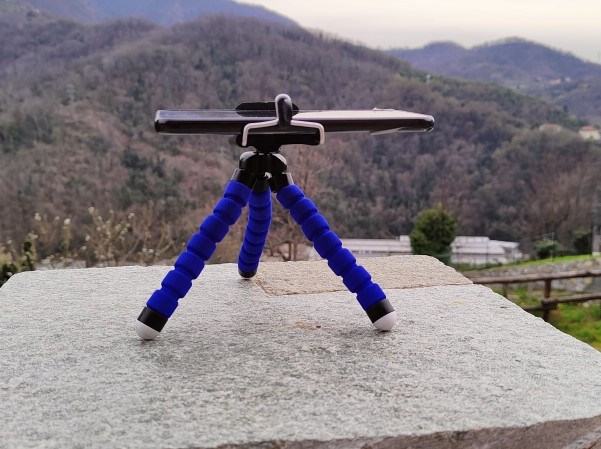
\includegraphics[width=0.27\textwidth]{fig/test2_position1.jpg}} 
    \subfigure[]{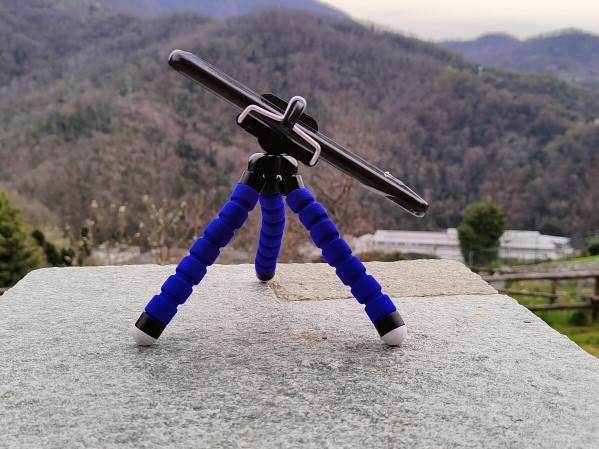
\includegraphics[width=0.27\textwidth]{fig/test2_position2.jpg}} 
    \subfigure[]{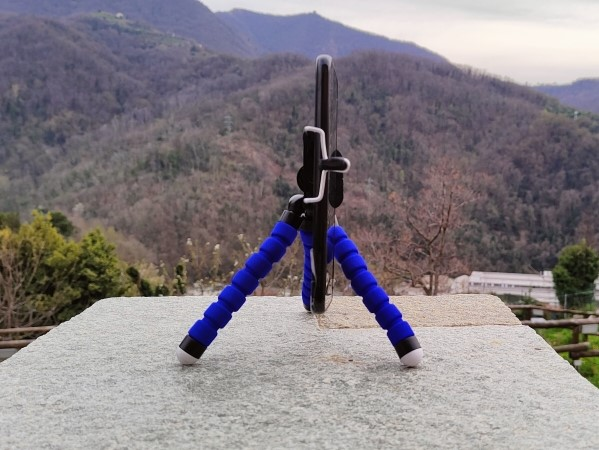
\includegraphics[width=0.27\textwidth]{fig/test2_position3.jpg}} 
    \newline
    \subfigure[]{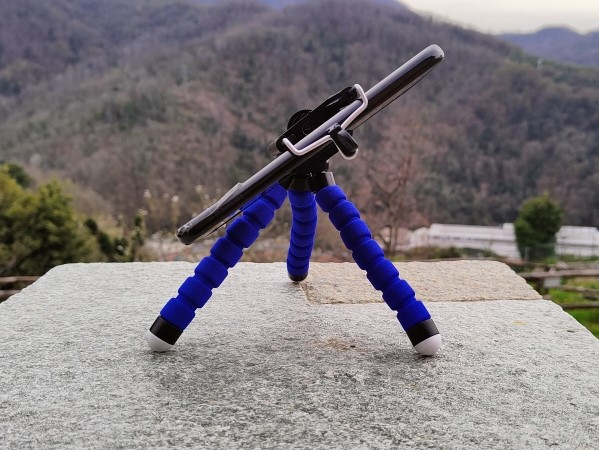
\includegraphics[width=0.27\textwidth]{fig/test2_position4.jpg}} 
    \subfigure[]{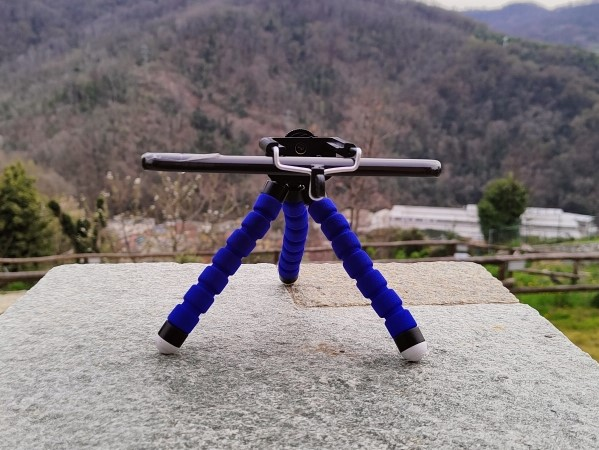
\includegraphics[width=0.27\textwidth]{fig/test2_position5.jpg}}    
    \caption{Test 2 acquisition with the smartphone in 5 different positions: (a) position 1 (b) position 2 (c) position 3 (d) position 4 (e) position 5}
    %\label{fig:foobar}
	\label{FIG:test2_setup} 
\end{figure}
As shown in the figure \ref{FIG:test2_setup}a, in position 1 the smartphone was oriented towards North and 
positioned horizontally, screen facing upwards. In the second position (figure \ref{FIG:test2_setup}b),
the smartphone was still facing north, but tilted at an angle of 45 degrees to the horizon, and screen 
facing upwards. In the third position (figure \ref{FIG:test2_setup}c) the smartphone is placed vertically with 
screen facing south. In the fourth position (figure \ref{FIG:test2_setup}d), the smartphone was oriented to  south and 
tilted 45 degrees to the horizon,  screen facing downwards. 
The last acquisition (Fig. \ref{FIG:test2_setup}e) was performed with the smartphone oriented to  south, 
placed horizontally, and screen facing downwards. 
The test was performed, in Manesseno (Genoa) on the 20\textsuperscript{th} of March 2020. 
Each acquisition lasted about half an hour in the following sequence:
\begin{itemize}
    \item position 1: from 15:20 to 15:50 UTC
    \item position 2: from 15:50 to 16:24 UTC
    \item position 3: from 16:32 to 16:57 UTC
    \item position 4: from 17:11 to 17:48 UTC
    \item position 5: from 17:48 to 18:21 UTC
\end{itemize}
\subsection{Test 3: Pedestrian Navigation}
Navigation is one of the main areas in which the GNSS receiver embedded into a smartphone is employed. 
Test 3 aims of making an assessment of the performance of the GNSS positioning from a smartphone in a typical 
scenarios such as  pedestrian navigation. 
More specifically, test 3 consists of a kinematic pedestrian acquisition involving two GNSS receivers: 
the Xiaomi Mi 8, and the Stonex S500, used as a term of comparison. The Stonex S500 is a single frequency (L1) 
and multi constellation (GPS, GLONASS, Galileo, and BeiDou) typically used for GIS (Geographic Information System) 
and RTK applications. 
The test was carried out on the 19\textsuperscript{th} of December 2021 in Genoa in Piazzale San Francesco d'Assisi, 
on a known path. The test path, shown in the figure \ref{FIG:test3_setup}a, was identified by determining the vertices of a 
square. In order to get the vertexes' coordinates with high precision, the four vertexes were surveyed in NRTK modality with 
the Stonex S70G, a geodetic level GNSS receiver, and exploiting the Ligurian NRTK network for getting the differential 
corrections. Once surveyed the vertexes were materialised using four targets. 
\begin{figure}[H] 
	\centering
    \subfigure[]{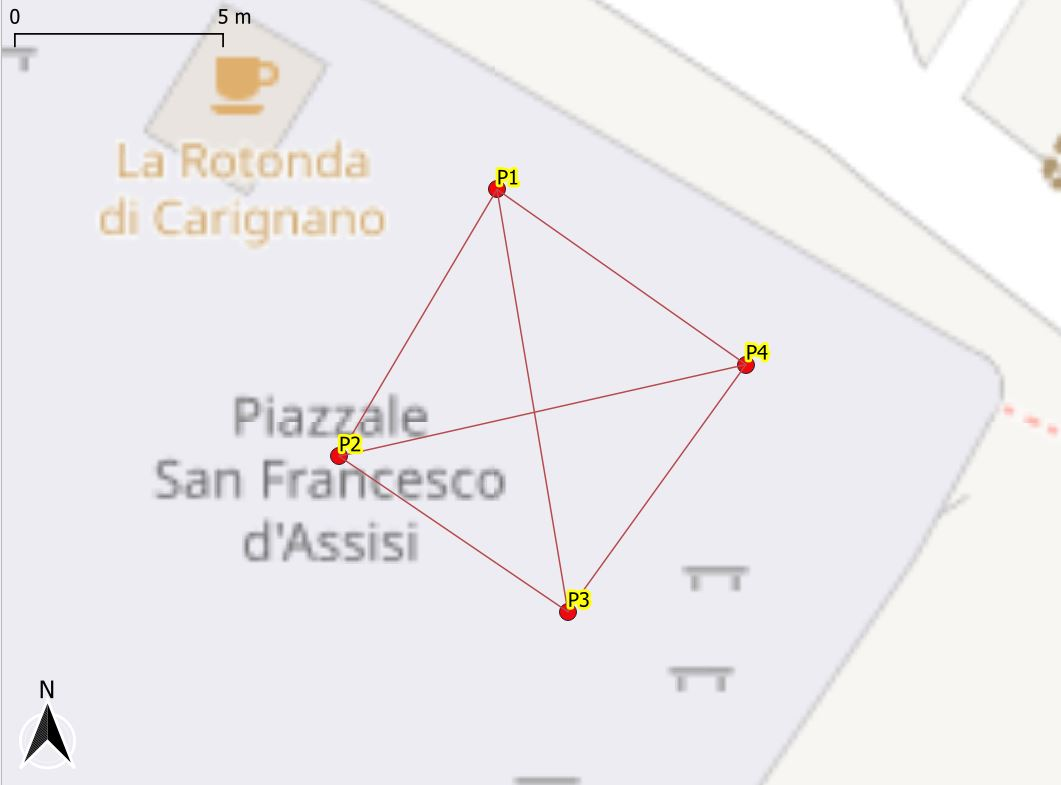
\includegraphics[width=0.48\textwidth]{fig/percorso_test3.jpg}} 
    \subfigure[]{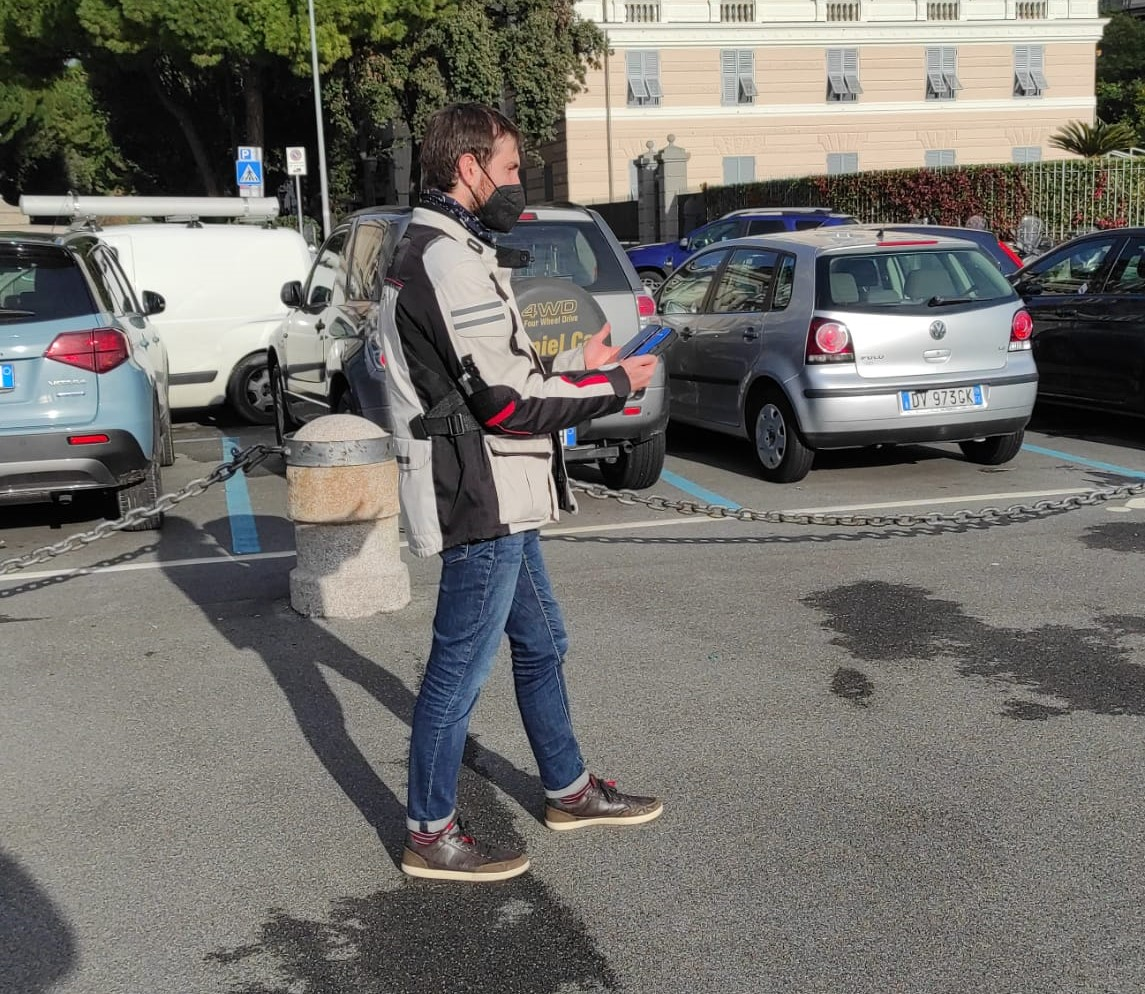
\includegraphics[width=0.48\textwidth]{fig/test3_walk.jpg}} 
    \caption{(a) Path used for test 3 (b) Test 3 execution}
    %\label{fig:foobar}
	\label{FIG:test3_setup} 
\end{figure}
Test 3 started at vertex number 1 with a static acquisition of 2 minutes. 
After that a walk between the four vertexes was performed along the squared sides as depicted in Fig. \ref{FIG:test3_setup}a. 
Each side has been traversed in both directions (e.g. from vertex 1 to vertex 2 and from vertex 2 to vertex 1). 
The test ended at vertex 1 with a static acquisition of 2 minutes. Data from both the receivers were collected at 
1 Hz rate. During the test, the two receivers were held at a height of about 1 metre above the 
ground (see Fig. \ref{FIG:test3_setup}b).
\subsection{Test 4: Multipath Effect}
Multipath and other interferences are one of the main source of error in GNSS positioning in urban canyons, 
especially if mass market GNSS receivers are employed. Based on this consideration, test 4 aims in evaluating 
the impact of multipath  in smartphone positioning. Similarly to test 3, a second GNSS receiver is used for comparing 
positioning results. Test 4 consists then in static acquisition, in which, for a specific interval, the multipath effect 
was reproduced by placing a metal plate behind the receivers (see figure \ref{FIG:test4_setup}).

The receivers used in this test are the Xiaomi Mi 8, and the ublox ZED F9P coupled with the AN-MB-00 patch antenna. The ublox ZED F9P is a mass market multi-frequency (L1/L2) and multi-constellation (GPS, GLONASS, Galileo, and BeiDou) GNSS receiver.

\begin{figure}[H] 
	\centering
    \subfigure[]{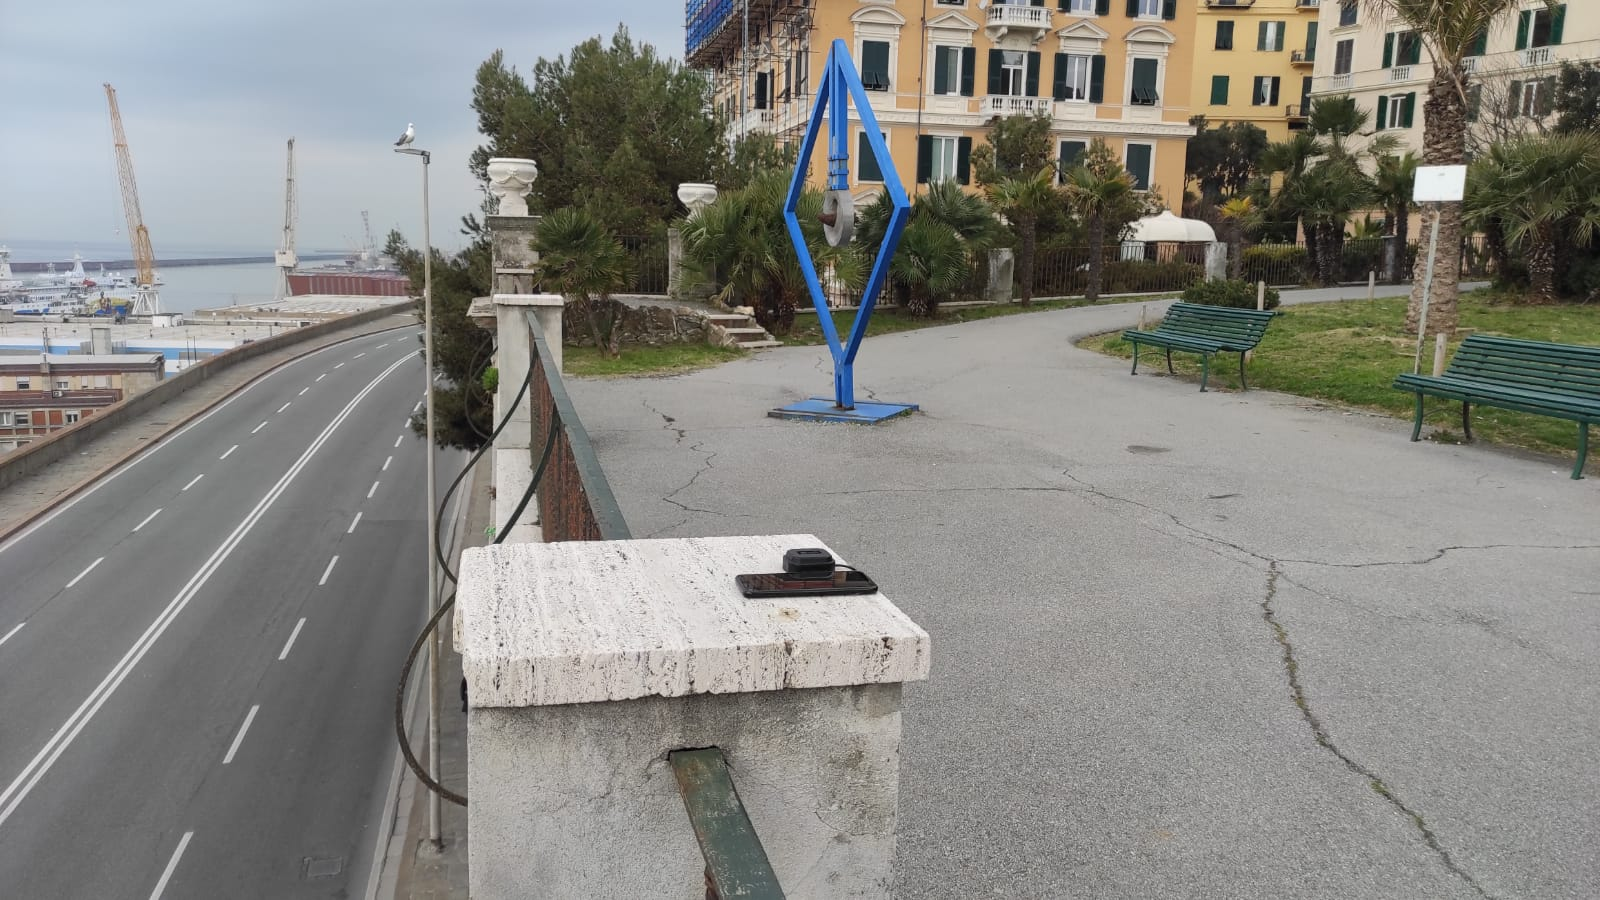
\includegraphics[width=0.48\textwidth]{fig/test4_standard.jpg}} 
    \subfigure[]{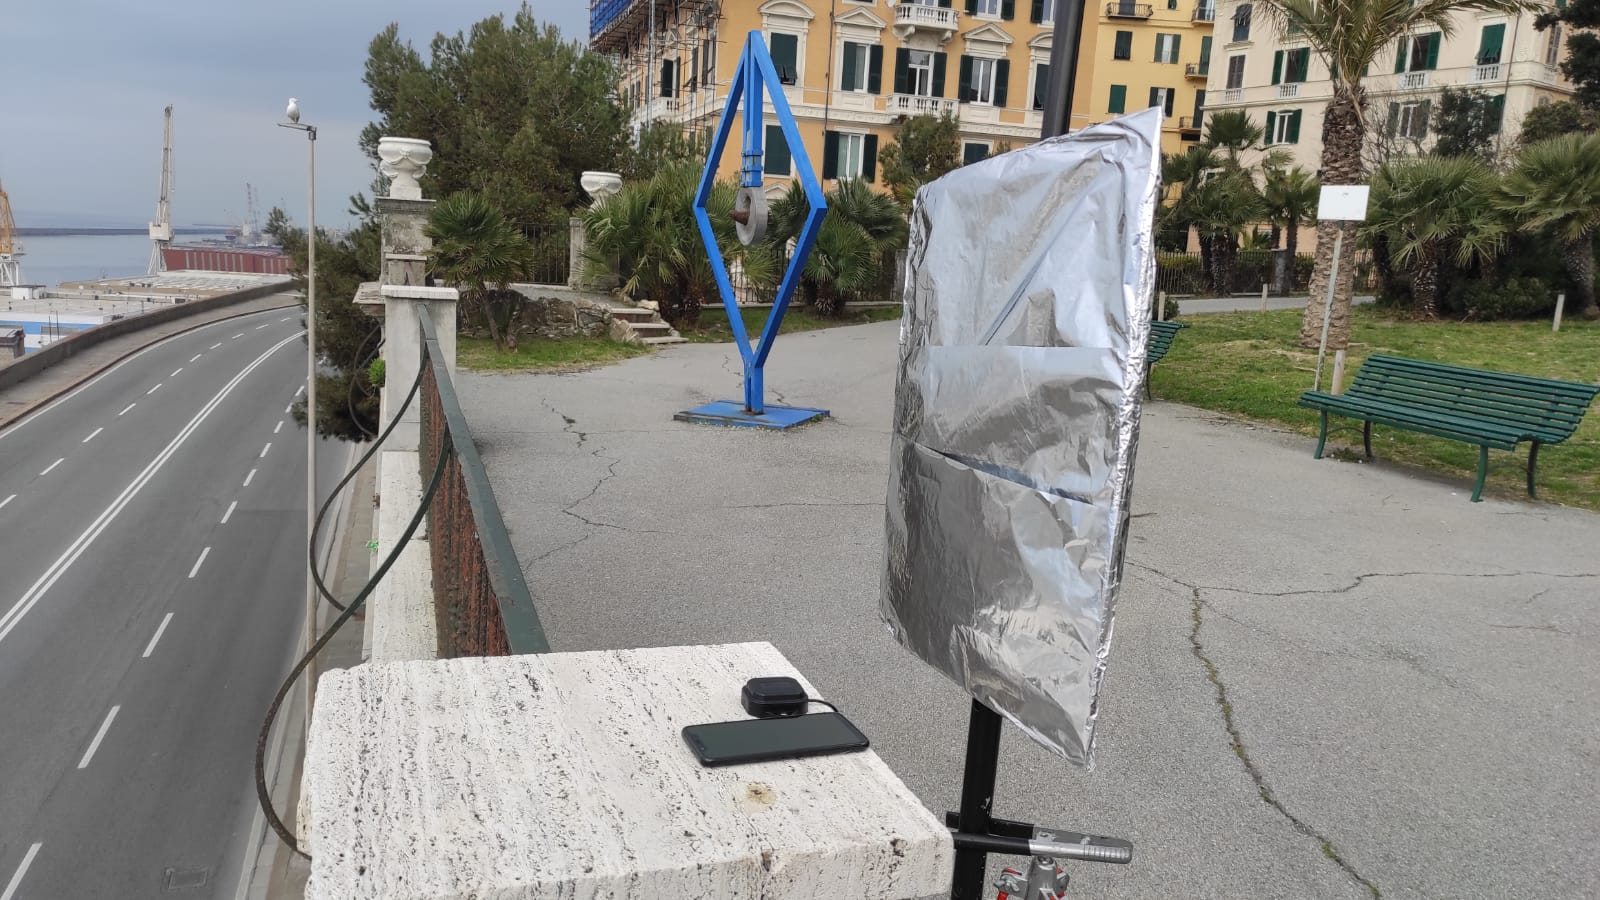
\includegraphics[width=0.48\textwidth]{fig/test4_multipath.jpg}} 
    \caption{Test 4 acquisition under standard condition (a), and with multipath induced (b)}
   % \label{fig:foobar}
	\label{FIG:test4_setup} 
\end{figure}

Test 4 was performed in Villa Croce (Genoa) on the 10\textsuperscript{th} of March 2022. 
The two receivers were placed in a point whose coordinates were determined with high precision in NRTK modality using  the Stonex S70G receiver, and exploiting the Ligurian NRTK network for the differential corrections. The static acquisition started at 9:15 am UTC time and lasted 1 hour. From 9:45 to 10:00 the multipath effect was induced placing the metal plate behind the receivers (see Fig. \ref{FIG:test4_setup}). After 10:00 the plate was removed and the acquisition ended at 10:15. Data from both the receiver were 
collected at 1 Hz rate.

\section{Discussion}
In this section the test results together with the adopted processing strategies are explained in details. Before proceeding to the discussion of the results, it's useful to clarify the concepts of precision and accuracy of the measurements, which are two parameters used to evaluate the positioning performances. Accuracy refers to the degree of dispersion of individually measured data with respect to the mean value of the series to which they belong to. Precision, on the other hand, means the deviation between the measured data and the real or reference data (i.e. the precise coordinates of the point). Figure \ref{FIG:prec_vs_acc} illustrates the difference between precision and accuracy for a generic data set.

\begin{figure}[H] 
	\centering
	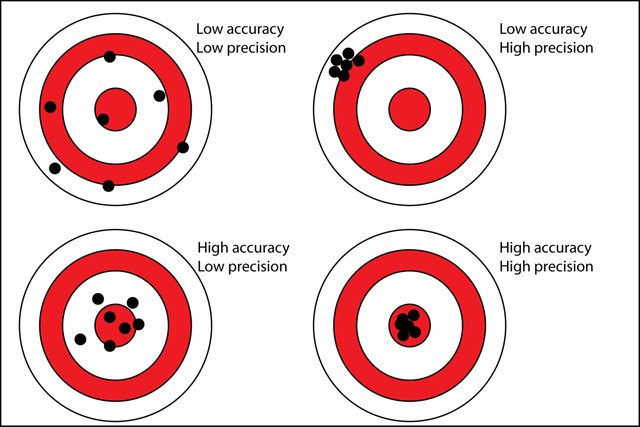
\includegraphics[scale=0.4]{fig/Precision-versus-accuracy.jpg} 
	\caption{Precision vs Accuracy}
	\label{FIG:prec_vs_acc} 
\end{figure}

Considerations on accuracy and precision of the solution can be made through the Standard Deviation (STD) and Root Mean Square (RMS) values. Given a set of elements STD and RMS can be defined as:

\begin{equation} 
	\begin{matrix} 
		STD= \sqrt{\frac{1}{N}\cdot \sum_{k=1}^N \left(x_{k}-\mu_{x}\right)^2 }\\ 
		RMS= \sqrt{\frac{1}{N}\cdot \sum_{k=1}^N \left(x_{k}-\tilde{x} \right)^2 }
		\end{matrix}
	\\
	\label{eq:std-rms}
\end{equation}
Where:
\begin{itemize}
\item $N$ is the total number of elements,
\item $x_{k}$ is a generic element belonging to the set,
\item $\mu_{x}$ is the mean value,
\item $\tilde{x}$ is a reference value for the elements (i.e., in this case, the precise coordinates of the point).
\end{itemize}

Given their definition, the STD can be considered an indicator of the precision, while the RMS can be considered an indicator of the accuracy.

\subsection{Processing Strategy}


All the processing exposed in this chapter were performed using the RTKLIB v 2.4.3 b34 software. In order to evaluate both accuracy and precision  accuracy the static tests processed as kinematic ones, i.e. obtaining as output a point cloud, with the coordinates computed epoch by epoch. Mainly two type of processing are performed: a Stand Alone positioning, which requires only the observable of the receiver in exam and a relative post processing which involves not only the observables of the receiver in exam but also the ones of a base station. This second processing is also called Post-Processed Kinematics (PPK). Unless otherwise specified the options used for processing are the following. 
The Ionosphere and Troposhere models used are the Klobuchar \cite{Klobuchar:1987} (which parameters are transmitted with the navigation message) and Saastamoinen \cite{Saastamoinen} respectively. For every tests only the broadcast ephemeris were considered and an elevation mask of \ang{15} is also set. 

Concerning the PPK elaborations the solution type combined was set. This options refers to the direction in time that the Kalman filter is run and its possible values are forward, backward and combined. Forward is the the only mode that can be used in real-time solutions (RTK). In this modality, the observation data is processed through the Kalman filter in the forward direction, i.e. starting with the beginning of the data and continuing through to the end. Backward mode is the opposite,  data is run through the filter starting with the end of the data and continuing to the beginning. In Combined mode, the filter is run both ways and the two results are combined into a single solution.


\subsection{Test 1}
In order to understand both the impact of the measurement noise in the positioning and quality of the positioning retrieved from the smartphone with respect to a geodetic receiver, two processing were computed: a Stand Alone, and a Post Processing with a common base receiver. In the Stand Alone processing only the pseudorange measurement are considered, and the two receiver are processed independently of each other. In order to make the results comparable, the constellation envolved in the processing were GPS and GLONASS, as GENU receiver was not able to track also Galileo and BeiDou as the smartphone. A cut off angle of \ang{15} was set for both the receivers. The chosen data rate for this elaboration is 1 Hz.
The results of the Stand Alone positioning for the two receivers are shown in Fig. \ref{FIG:test1_standalone}

\begin{figure}[H] 
	\centering
    \subfigure[]{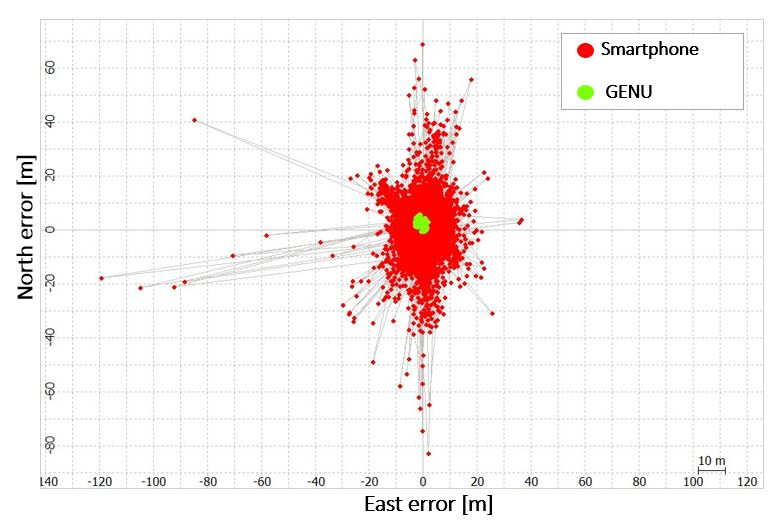
\includegraphics[width=0.48\textwidth]{fig/test1/test1_stand_alone_groundtrck.jpg}} 
    \subfigure[]{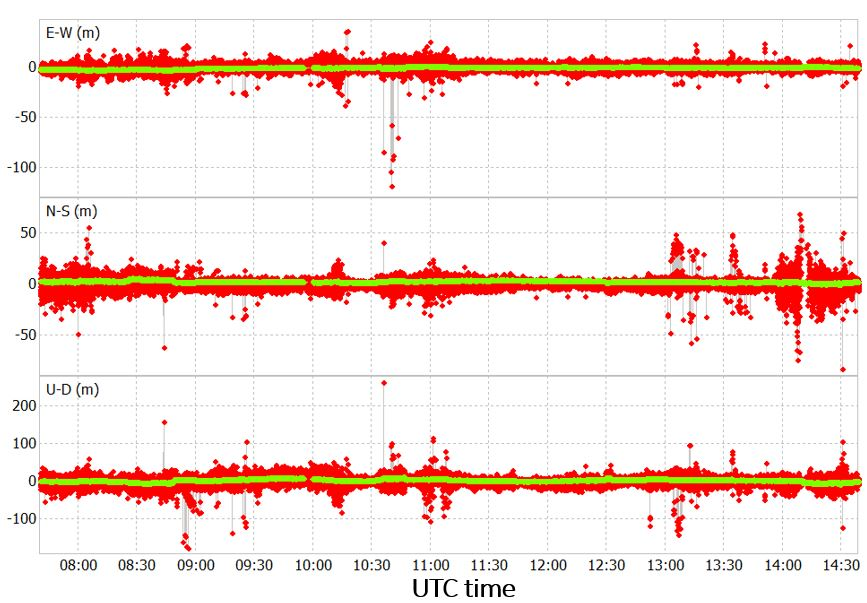
\includegraphics[width=0.48\textwidth]{fig/test1/test1_stand_alone_timeserie.jpg}} 
    \caption{(a) Scatter plot of the positioning error for GENU (green) and Smartphone (red) receivers  (b) time series of the positioning error for GENU (green) and Smartphone (red) receivers}
    %\label{fig:foobar}
	\label{FIG:test1_standalone} 
\end{figure}

The values reported in Fig. \ref{FIG:test1_standalone} refers to the difference computed with respect to the precise coordinates for both the receivers. 
The statistics values, in terms of RMS and standard deviation, of such differences are reported in tab \ref{tab:test1_spp}.

\begin{table}[H]
	\centering
	\begin{tabular}{|c|p{1.5cm}|p{1.5cm}|p{1.5cm}|p{1.5cm}|p{1.5cm}|p{1.5cm}|}
	\hline
	\textbf{Receiver} & \textbf{RMS E [m]} & \textbf{RMS N [m]} &
	\textbf{RMS H [m]} &\textbf{STD E [m]}&\textbf{STD N [m]}&\textbf{STD H [m]}\\
    \hline
	GENU & 2.385 & 1.278& 3.729&0.965&0.884&3.441\\  
    \hline
	Smartphone & 4.207 & 5.723& 12.784&3.916&5.643&12.784\\ \hline
	\end{tabular} 
	\caption{Test 1, Stand Alone processing results}
	\label{tab:test1_spp}
\end{table}

With reference to the values in the Table \ref{tab:test1_spp} and Fig. \ref{FIG:test1_standalone} it is possible to state that the geodetic receiver and the smartphone presents a meter level accuracy, which is typical of this kind of positioning. The accuracy of the smartphone positioning however results definitely coarser than the one of the geodetic receiver. Also concerning the precision, the smartphone presents coarser results. Some outilers of the order of several tens of metres can also be detected between the smartphone positions. This behaviour can be explained by the poor quality of the smartphone observables compared to those of the geodetic receiver. An indicator of the quality of observables is the residual of the pseudorange measurements. The pseudorange residual is the difference between the value of the satellite-receiver range, computed a-posteriori (when the point coordinates are known) and the observed value. The residual plot for the two receivers in shown in Fig. \ref{FIG:test1_psdrgres}

\begin{figure}[H] 
	\centering
    \subfigure[]{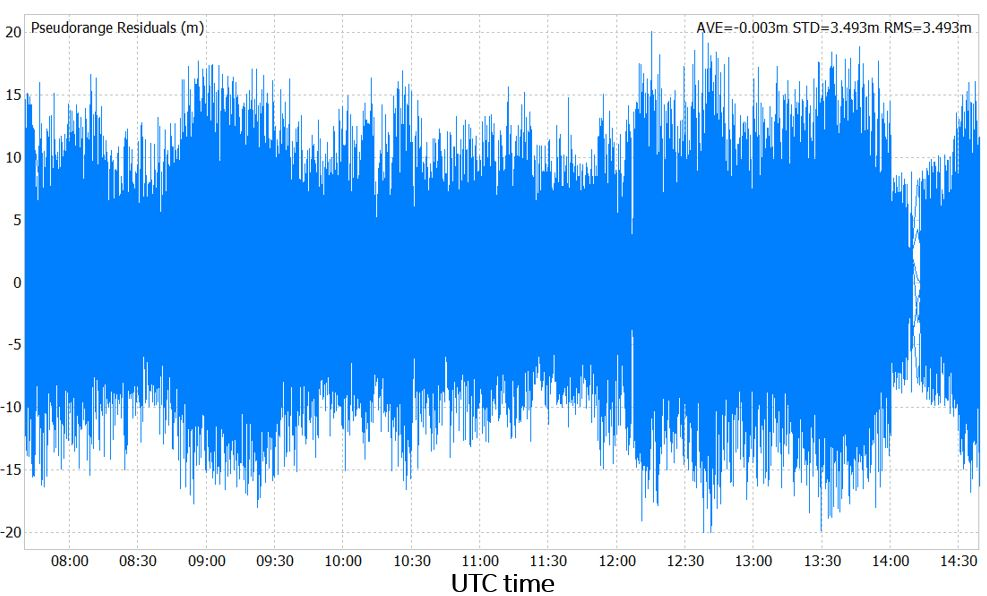
\includegraphics[width=0.48\textwidth]{fig/test1/test1_psdrg_residual_xiaomi.jpg}} 
    \subfigure[]{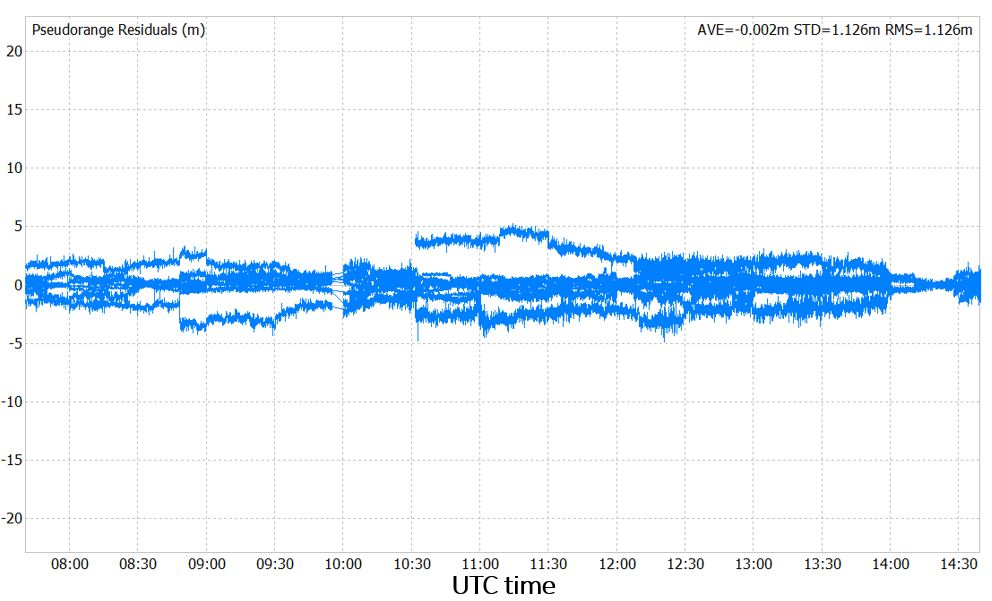
\includegraphics[width=0.48\textwidth]{fig/test1/test1_psdrg_residual_genu.jpg}} 
    \caption{(a) Residual pseudorange plot for Smartphone receiver (b) Residual pseudorange plot for GENU receiver}
   % \label{fig:foobar}
	\label{FIG:test1_psdrgres} 
\end{figure}

It is possible to state form Fig. \ref{FIG:test1_psdrgres} that pseudorange residuals from smartphone are definitely noisier than the ones from the GENU receiver. This can be explained by the different quality of the antennas which the two receivers mounts: GENU receiver in fact has a choke ring antenna, which is used for precise positioning purposes while the smartphone has an integrated antenna not specifically designed for GNSS positioning.    

Test 1 receivers have been also post processed with a common reference station. The base receiver chosen is GENO, a GNSS receiver of the RDN (Rete Dinamica Nazionale)\footnote{\url{https://www.igmi.org/it/direzione-geodetica}} located approximately 3 km away from the test field.

The obtained results are shown in figure \ref{FIG:test1_pp}

\begin{figure}[H] 
	\centering
    \subfigure[]{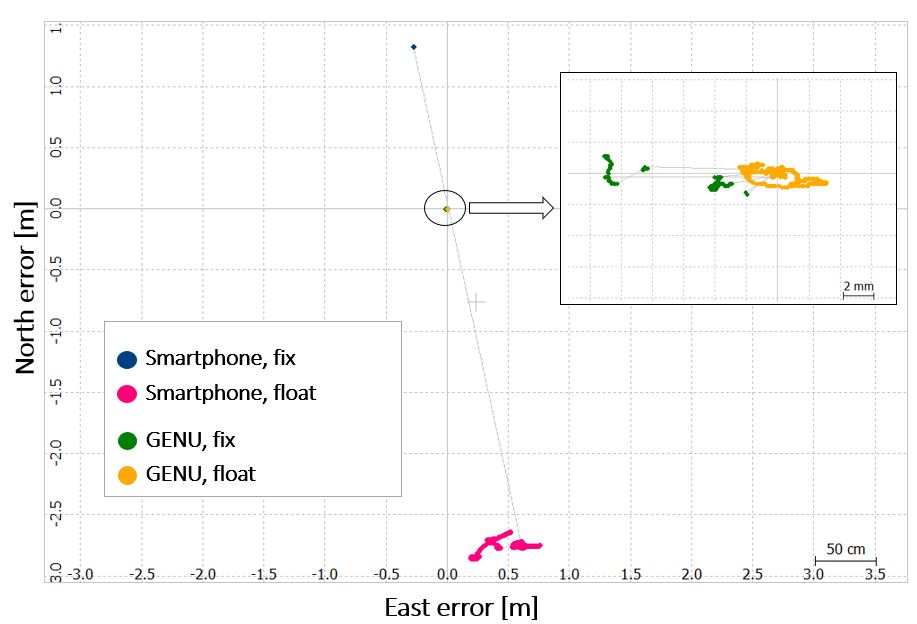
\includegraphics[width=0.48\textwidth]{fig/test1/test1_pp_groundtrck.jpg}} 
    \subfigure[]{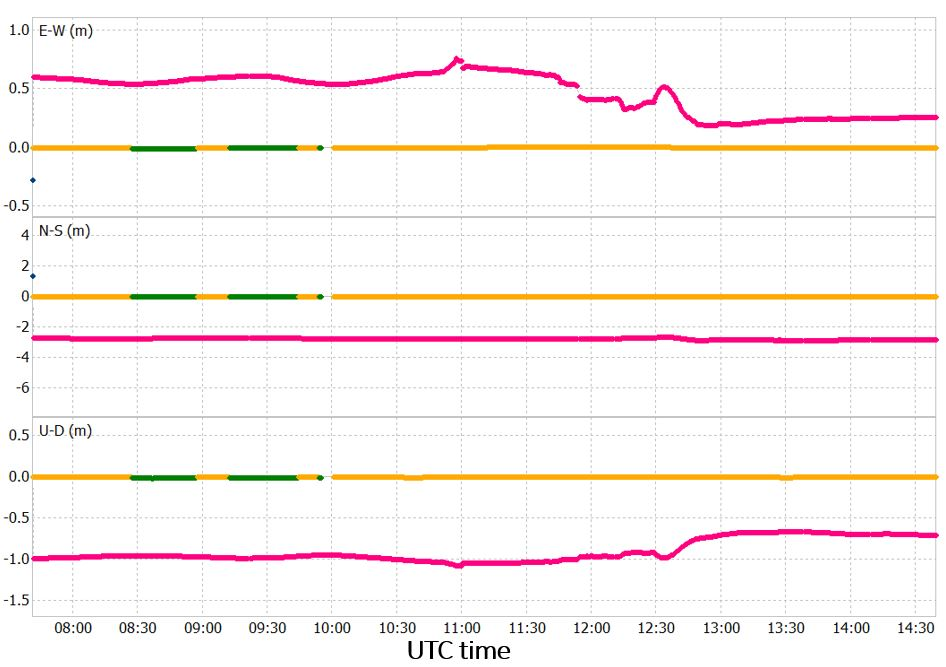
\includegraphics[width=0.48\textwidth]{fig/test1/test1_pp_timeserie.jpg}} 
    \caption{(a) Scatter plot of the positioning error for GENU (green) and Smartphone (red) receivers  (b) time series of the positioning error for GENU (green) and Smartphone (red) receivers}
    %\label{fig:foobar}
	\label{FIG:test1_pp} 
\end{figure}

The statistics values, in terms of RMS and standard deviation with respect to the precise coordinates of the receivers, are reported in Table \ref{tab:test1_pp}

\begin{table}[H]
	\centering
		\begin{tabular}{|c|p{1.5cm}|p{1.5cm}|p{1.5cm}|p{1.5cm}|p{1.5cm}|p{1.5cm}|}
	\hline
	\textbf{Receiver} & \textbf{RMS E [m]} & \textbf{RMS N [m]} &
	\textbf{RMS H [m]} &\textbf{STD E [m]}&\textbf{STD N [m]}&\textbf{STD H [m]}\\
	\hline
	GENU & 0.004 & 0.001 & 0.005&0.003&0.0004&0.003\\  
    \hline
	Smartphone & 0.576 & 0.242& 0.333&0.167&0.152&0.158\\ \hline
	\end{tabular} 
	\caption{Test 1, Post processing results}
	\label{tab:test1_pp}
\end{table}

The GENU receiver has an RMS in the order of millimetres for all the components. The standard deviations in East, North and Height components are also in the millimetre range. Those are expected results for a geodetic GNSS receivers. The smartphone receiver in the other hand presents coarser results with respect to the geodetic one. The RMS are in the order of tens of centimeters with a maximum of 58 cm in the East. Also the standard deviations is in the order of tens of centimeters with a maximum in the Height component equal to 17 cm.      
The two positioning can be also compared in terms of percentage of fixing solutions obtained. The smartphone positioning only have 1 fixing solution (i.e. 0.1\%) while GENU receiver have 127 fixing solutions (i.e. 15.4\%). Furthermore the only fixing solution of the smartphone (blue point in Fig. \ref{FIG:test1_pp}a  can be considered an outlier as its error values are not coherent with the rest of the obtained errors. It's error components for East, North and Height components in fact are -1.306 m, 3.899 m and 2.753 m respectively with respect to the precise coordinates of the point. Considering that for fixed solutions the expected errors are in the order of few centimeters, this point can be also considered a false fixed solution.   

\subsection{Test 2}
Similarly to test 1, also for test 2 two processing were computed in order to evaluate whether the smartphone orientation influences the positioning results. The first one is a Stand Alone processing and the second one is a PPK processing with GENU receiver. The baseline between the smartphone receiver and the GENU base, in this case is about 10 km. Considering the length of the baseline and the low quality of smartphone hardware in this case it was not possible to determine the precise coordinates of the smartphone. Considering that and than only consideration concerning the precision and not the accuracy can be carried out for this case study. Nevertheless it interesting to report this case also to show the behaviour of relative positioning from smartphone considering long baselines.

The result for the Stand Alone processing are exposed in Fig. \ref{FIG:test2_sa_scatter}:

\begin{figure}[H] 
	\centering
    \subfigure[]{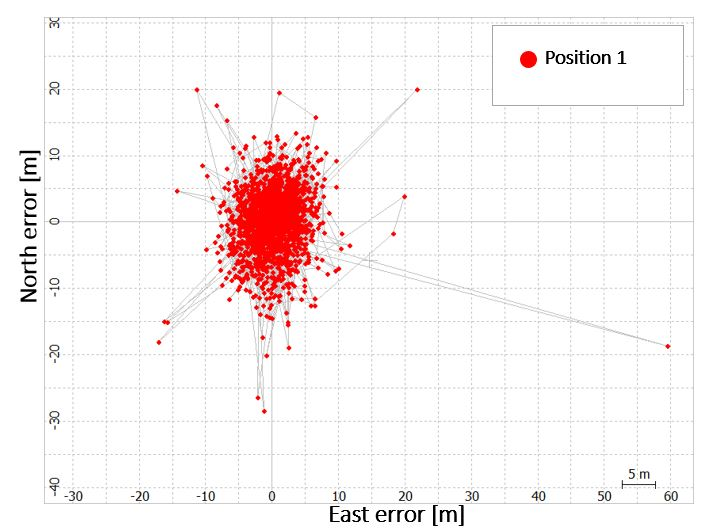
\includegraphics[width=0.3\textwidth]{fig/test2/test2_p1_sa.jpg}} 
    \subfigure[]{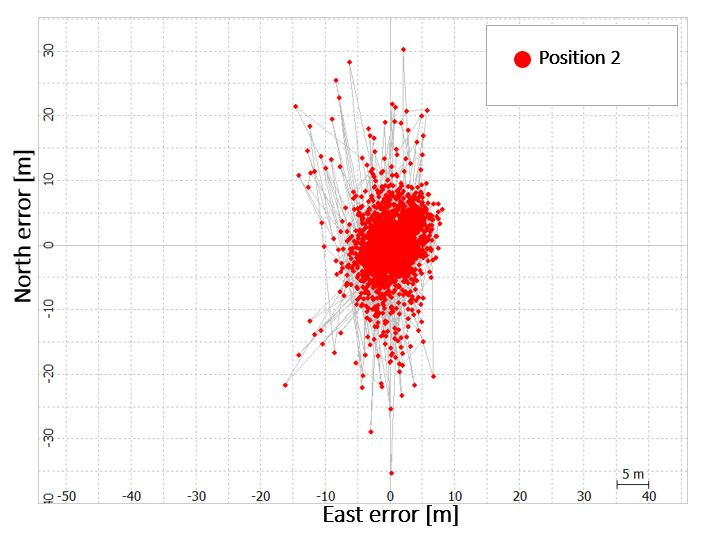
\includegraphics[width=0.3\textwidth]{fig/test2/test2_p2_sa.jpg}} 
    \subfigure[]{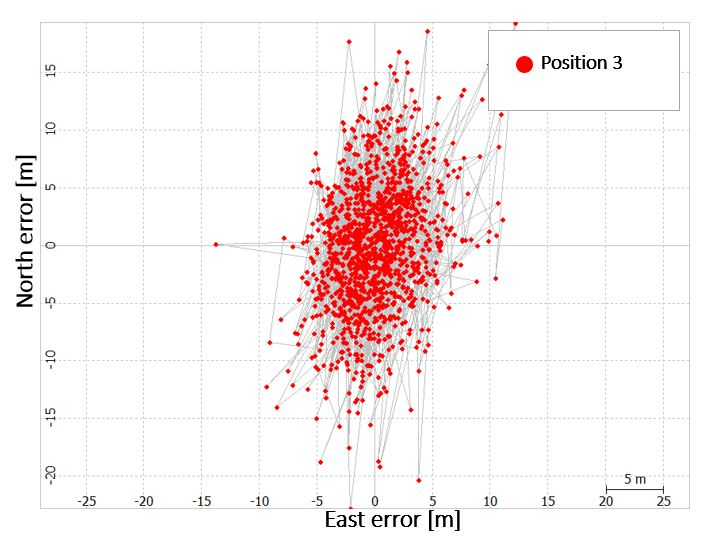
\includegraphics[width=0.3\textwidth]{fig/test2/test2_p3_sa.jpg}} 
    \newline
    \subfigure[]{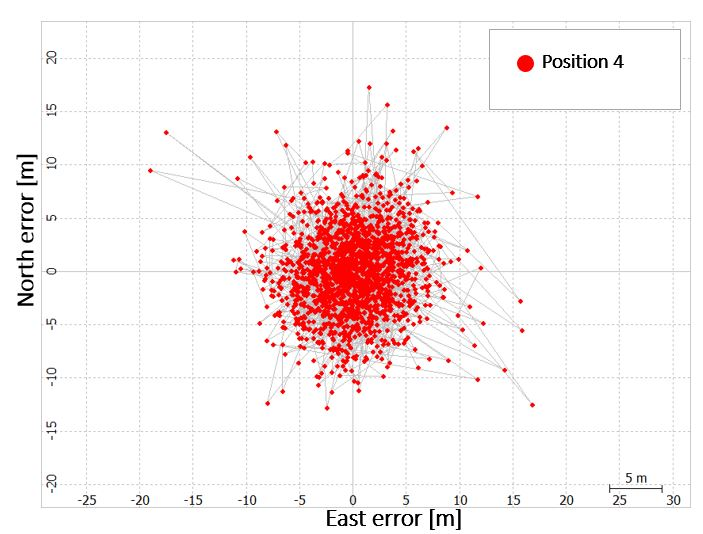
\includegraphics[width=0.3\textwidth]{fig/test2/test2_p4_sa.jpg}} 
    \subfigure[]{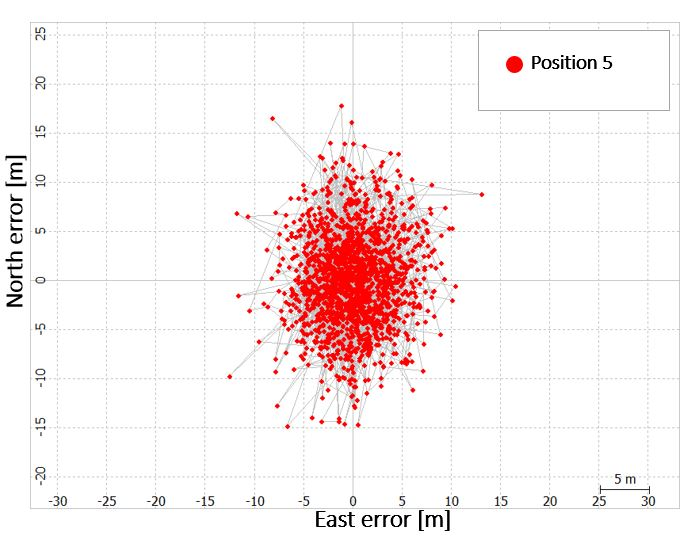
\includegraphics[width=0.3\textwidth]{fig/test2/test2_p5_sa.jpg}}    
    \caption{Scatter plot of the positioning error for test 2 in Stand Alone modality: (a) position 1 (b) position 2 (c) position 3 (d) position 4 (e) position 5}
   % \label{fig:foobar}
	\label{FIG:test2_sa_scatter} 
\end{figure}

Table \ref{tab:test2_sa} shows the standard deviation for the position errors obtained:

\begin{table}[H]
	\centering
	\begin{tabular}{|c|c|c|c|}
	\hline
	\textbf{Position} &\textbf{STD E [m]}&\textbf{STD N [m]}&\textbf{STD H [m]}\\
    \hline
	 1 & 3.352 & 4.833  & 10.286\\  
    \hline
     2 & 3.040 & 5.455  & 7.391\\  
    \hline
     3 & 2.982 & 5.474  & 6.265\\  
    \hline
     4 & 3.572 & 3.857  & 14.188\\  
    \hline
     5 & 3.276 & 4.655  & 11.436\\  
    \hline
	\end{tabular} 
	\caption{Test 1, Post processing results}
	\label{tab:test2_sa}
\end{table}

The standard deviation values derived from the five different positions are in agreement with each other and settle at values of about 3 m in the East component, about 5 m in the North component and about 10 m in the Height component. These values are also of the same order of magnitude as those obtained for the Stand Alone positioning of test 1 (cfr Table \ref{tab:test1_spp}). Therefore, there does not seem to be one position that clearly prevails over another in terms of precision in smartphone Stand Alone positioning.

As previously stated nothing can be said about the positioning accuracy, as it was not possible to determine the precise coordinates of the smartphone.

The results of the PPK processing with GENU base are exposed in Fig. \ref{FIG:test2_pp_scatter} 

\begin{figure}[H] 
	\centering
    \subfigure[]{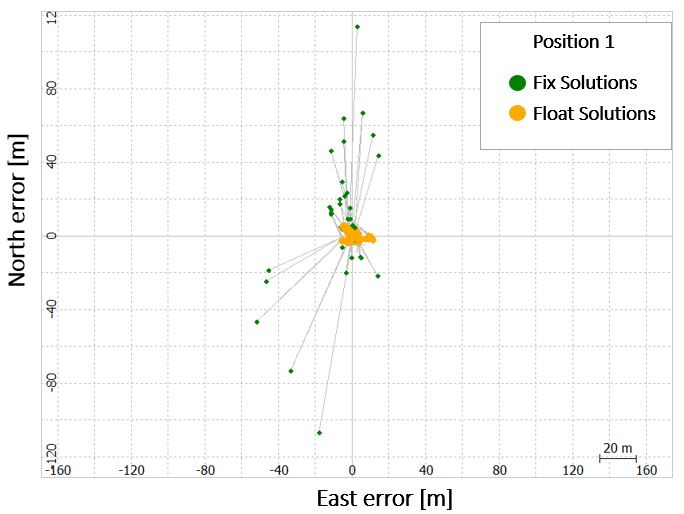
\includegraphics[width=0.3\textwidth]{fig/test2/test2_p1_pp.jpg}} 
    \subfigure[]{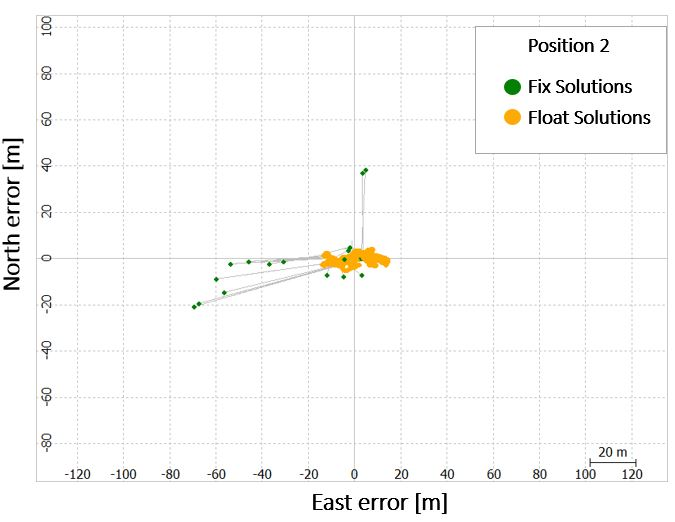
\includegraphics[width=0.3\textwidth]{fig/test2/test2_p2_pp.jpg}} 
    \subfigure[]{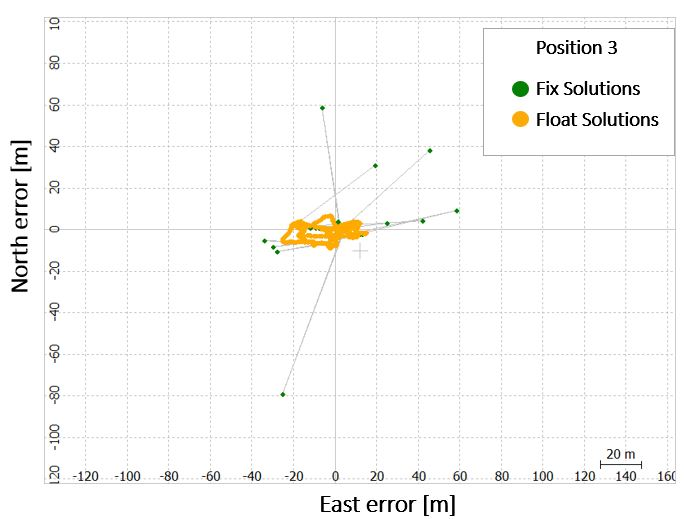
\includegraphics[width=0.3\textwidth]{fig/test2/test2_p3_pp.jpg}} 
    \newline
    \subfigure[]{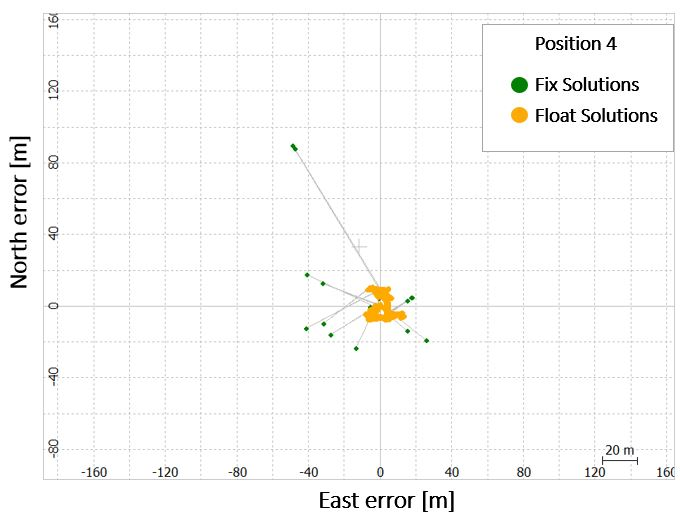
\includegraphics[width=0.3\textwidth]{fig/test2/test2_p4_pp.jpg}} 
    \subfigure[]{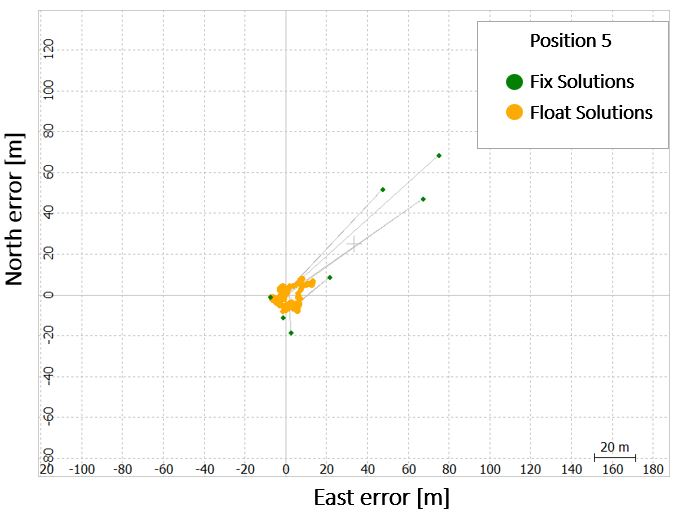
\includegraphics[width=0.3\textwidth]{fig/test2/test2_p5_pp.jpg}}    
    \caption{Scatter plot of the positioning error for test 2 in Post Processing: (a) position 1 (b) position 2 (c) position 3 (d) position 4 (e) position 5}
   % \label{fig:foobar}
	\label{FIG:test2_pp_scatter} 
\end{figure}

Table \ref{tab:test2_pp_fixflt} shows the standard deviation for the position errors obtained:

\begin{table}[H]
	\centering
	\begin{tabular}{|c|c|c|c|}
	\hline
	\textbf{Position} &\textbf{STD E [m]}&\textbf{STD N [m]}&\textbf{STD H [m]}\\
    \hline
	 1 & 4.017 & 6.061  & 9.282\\  
    \hline
     2 & 7.692 & 2.373  & 3.896\\  
    \hline
     3 & 9.854 & 4.217  & 9.365\\  
    \hline
     4 & 4.834 & 5.732   & 7.379 \\  
    \hline
     5 & 5.168 &  4.316& 9.925\\  
    \hline
	\end{tabular} 
	\caption{Test 1, Post processing results}
	\label{tab:test2_pp_fixflt}
\end{table}

From the graphs shown in the Fig. \ref{FIG:test2_pp_scatter} and the values in the Table \ref{tab:test2_pp_fixflt}, it can be state that PPK from smartphones on long baselines has precision errors in the order of meters, while sub metric values are attended for this type of techniques. It can be also said that all the fixed solution obtained are false fixing solutions as their error values are clearly not coherent with the rest of the obtained errors. 
Factors explaining this behaviour are the poor quality of GNSS data from smartphones and the length of the baseline. For the rest of the tests carried out in this work only shorter baselines ($<$ 1 Km) are then considered.
Also considering the post processing approach, it seems that none of the positions tested shows better results if compared to the others. Based on this, for the rest of the tests carried out in this work, no further attention will be paid to the orientation of the smartphone.


\subsection{Test 3}


The performance of the smartphone GNSS receiver in a kinematic contest can be analysed at two different levels: preprocessing level and positioning level. In both cases to better understand its performance, the data coming from the smartphone (Xiaomi Mi 8) are compared with the ones coming from the Stonex S500 receiver, which is considered as a benchmark.

Concerning the preprocessing level the quality of the incoming signal for the two receiver is compared. A good indicator of the incoming signal quality is the Signal to Noise Ratio (SNR), which is measure of the strength of the desired signal relative to background noise. SNR expressed in DB-Hz presents high values for a good incoming signal, while low values for a bad signal. The SNR values for the two receivers used in test 3 are shown in Fig. \ref{FIG:test3_snr}.

\begin{figure}[H] 
	\centering
    \subfigure[]{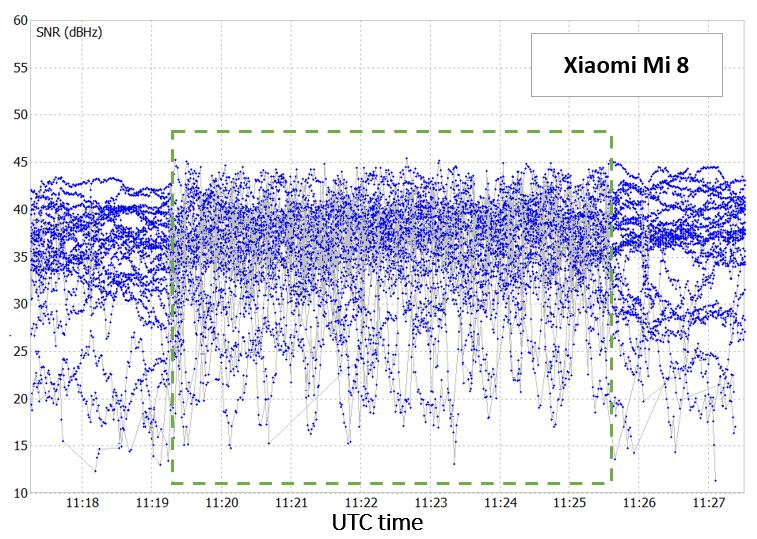
\includegraphics[width=0.48\textwidth]{fig/test3/test3_snr_xiaomi.jpg}} 
    \subfigure[]{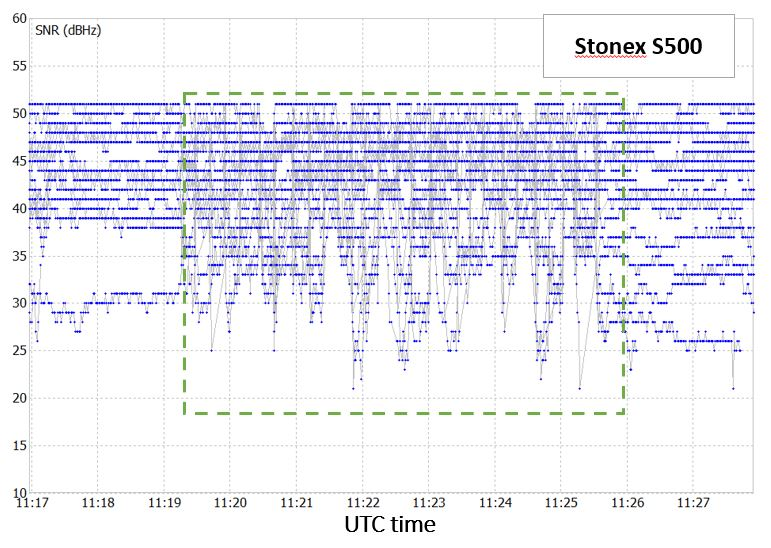
\includegraphics[width=0.48\textwidth]{fig/test3/test3_snr_s500.jpg}} 
    \caption{SNR for Xiaomi Mi 8 receiver (a) and for Stonex S500 receiver (b) }
    %\label{fig:foobar}
	\label{FIG:test3_snr} 
\end{figure}

Figure \ref{FIG:test3_snr} shows that the Stonex S500 receiver has a much better SNR than the Xiaomi Mi 8 receiver. In fact an average difference of about 10 DB-Hz between the two receivers is observed. From the SNR trend it's also possible to recognise the static and kinematic parts of the survey. The kinematic part, highlighted in the green dashed box, in fact presents a noisier SNR trend than the static parts located at the beginning at ad the end of the test.

It's also interesting to notice that number of satellites acquired by the two receivers (Fig. \ref{FIG:test3_nsat}).

\begin{figure}[H] 
	\centering
    \subfigure[]{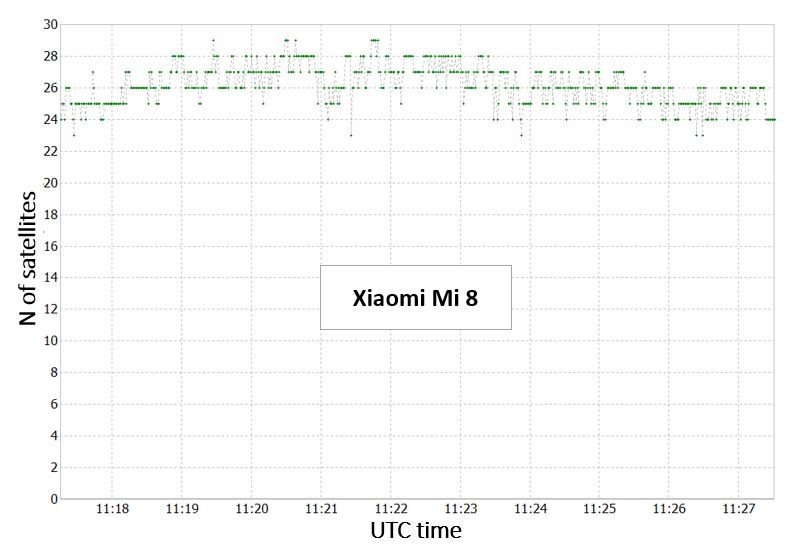
\includegraphics[width=0.48\textwidth]{fig/test3/test3_nsat_xiaomi.jpg}} 
    \subfigure[]{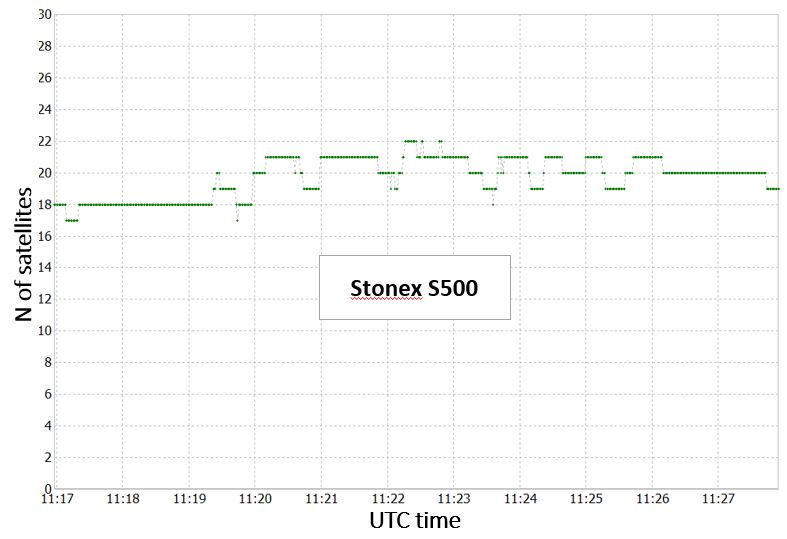
\includegraphics[width=0.48\textwidth]{fig/test3/test3_nsat_s500.jpg}} 
    \caption{Number of satellite observed by Xiaomi Mi 8 receiver (a) and Stonex S500 receiver (b) }
   % \label{fig:foobar}
	\label{FIG:test3_nsat} 
\end{figure}

The number of satellites observed by the Xiaomi Mi 8 is greater than that of the Stonex S500, but much more variable over time. In fact, the Xiaomi Mi 8 receiver also acquires very noisy satellites (SNR $<$ 25 DB-Hz) for short periods of time, which are ignored by the Stonex S500. However, acquiring a larger number of satellites is not always advantageous for positioning purposes, especially if the acquired signals are very noisy. 


Concerning the positioning part, both the receiver were post processed with a common GNSS permanent station located about 200 m away from the test field. This GNSS permanent station, hereafter called LIGE, was designed and realized in the ambit of this thesis work (see par \ref{par:lige}). LIGE permanent station is equipped with the low cost GNSS receiver Ublox ZED F9P coupled with the Hemisphere A45 antenna. 
For this case study the solution type "forward" is set in order to simulate a real time condition. 

The positioning solutions obtained are shown in Fig. \ref{FIG:test3_pp}.

\begin{figure}[H] 
	\centering
    \subfigure[]{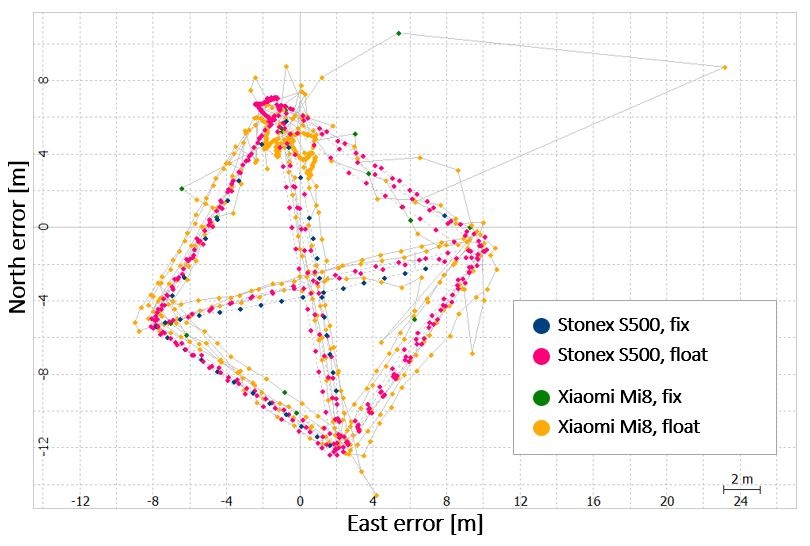
\includegraphics[width=0.48\textwidth]{fig/test3/test3_pp_scatter.jpg}} 
    \subfigure[]{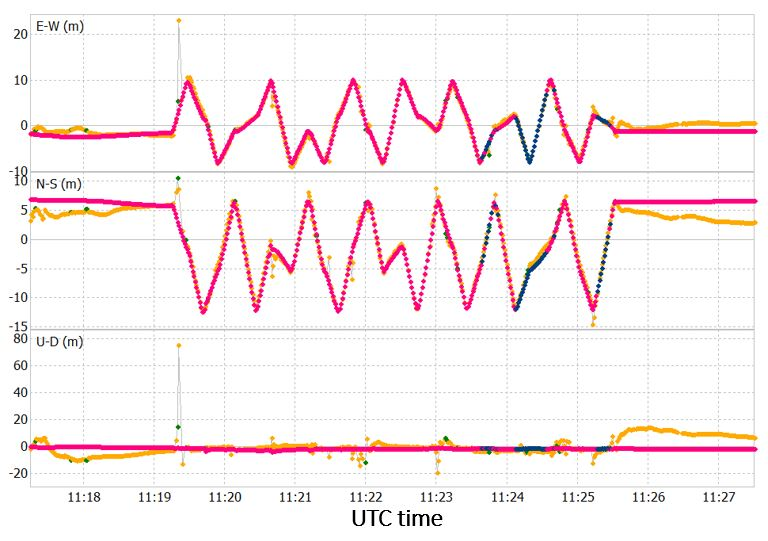
\includegraphics[width=0.48\textwidth]{fig/test3/test3_pp_timeserie.jpg}} 
    \caption{(a) Scatter plot of the positioning error for Xiaomi Mi8 and Stonex S500  (b) time series of the positioning error for Xiaomi Mi8 and Stonex S500}
   % \label{fig:foobar}
	\label{FIG:test3_pp} 
\end{figure}

Considering that the first two minutes and the last two minutes of the survey were carried out statically at vertex P1 (see Fig. \ref{FIG:test3_setup}), it is possible to make preliminary considerations on the accuracy of the positioning obtained by comparing the deviation of the positions obtained in the first two minutes and the last two minutes with respect to the precise coordinates of the vertex.
The Xiaomi Mi8 receiver presents and RMS of 1.066 m, 2.849 m and 5.670m for East, North and Height components respectively while the Stonex S500 has 0.598 m, 0.498 and 2.318 m for East, North and Height components respectively. The Stonex S500 receiver solution is therefore more accurate, especially when considering the North and Altitude components.


The two solutions can be compared also in terms of number of computed positions and percentage of fix and float solutions (see Table \ref{tab:test3_pp_quality}).

\begin{table}[H]
	\centering
	\begin{tabular}{|c|c|c|c|}
	\hline
	\textbf{Receiver} &\textbf{Number of solutions}&\textbf{Fixed solutions}&\textbf{Float solutions}\\
    \hline
	 Xiaomi Mi 8 & 595 & 19 (3,2\%) & 576 (96.8\%)\\  
    \hline
     Stonex S500 & 617 & 47 (7,6\%) & 570 (92.4\%)\\  
    \hline
	\end{tabular} 
	\caption{Test 3, Solution quality}
	\label{tab:test3_pp_quality}
\end{table}

The Xiaomi Mi 8 receiver presents fewer solutions than the Stonex S500. The poor quality of the GNSS measurement from the smartphone prevents the computation of the positioning for some epochs. Furthermore the Xiaomi Mi 8 solution, coherently with other results obtained from the previous tests presents some outliers and false fixing solutions.


\subsection{Test 4}
Similarly to test 3, also for this case the performance of the Xiaomi Mi8 receiver are compared to the ones of the other device involved, the Ublox ZED F9P in two different levels: preprocessing and positioning level. Once again in the preprocessing level the two receivers are compared in terms of quality of the incoming signal. For this purpose the SNR trend for the two receivers is shown in Fig. \ref{FIG:test4_snr}.
\begin{figure}[H] 
	\centering
    \subfigure[]{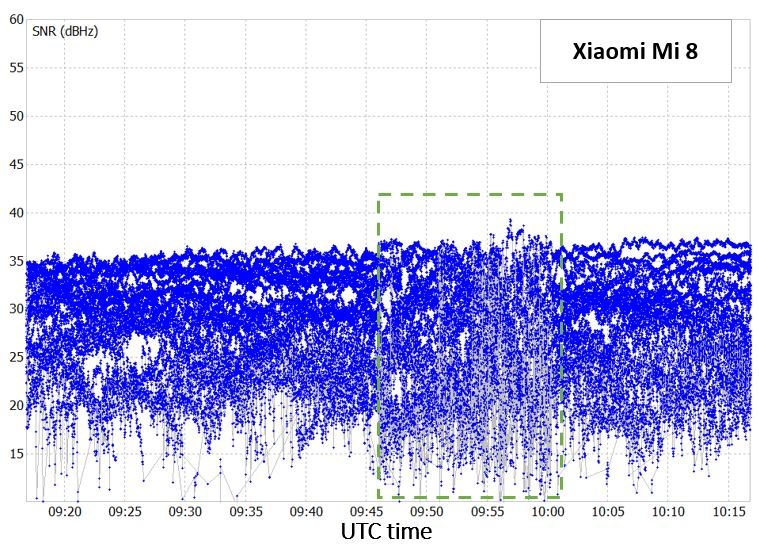
\includegraphics[width=0.48\textwidth]{fig/test4/test4_snr_xiaomi.jpg}} 
    \subfigure[]{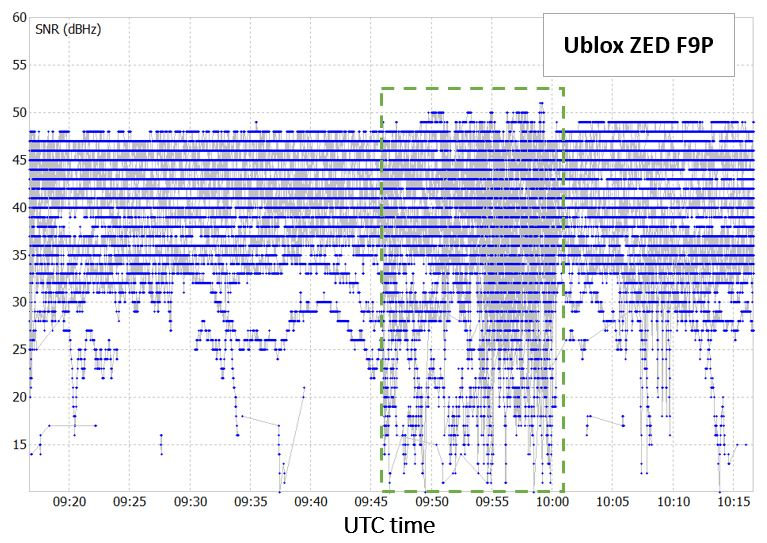
\includegraphics[width=0.48\textwidth]{fig/test4/test4_snr_ublox.jpg}} 
    \caption{SNR for Xiaomi Mi 8 receiver (a) and for Ublox ZED F9P receiver (b) }
  %  \label{fig:foobar}
	\label{FIG:test4_snr} 
\end{figure}

Concerning the SNR comparison, the results obtained for test 3 are confirmed also for this case study. The Xiaomi Mi 8 on average presents lower SNR values with respect to the Ublox ZED F9P. This means that, due to the poor quality of the smartphone's hardware, the signals acquired by the Xiaomi Mi 8 receiver are much noisier. From the SNR trend of the two receivers it's evident the period in which the multipath effect was induced with the metal plate, i.e. from 9:45 a.m. to 10:00 a.m. UTC (green boxes in Fig. \ref{FIG:test4_snr}). In this time interval, as expected, the signals acquired is degraded.This results in a general lowering of SNR values, and a significantly noisier trend. 


Concerning the positioning part, both the receiver were post processed with a the LIGE permanent station which is about 0.2 km away from the test field. Similarly to test 3 also for this case study the solution type chosen is forward. Figure \ref{FIG:test4_pp} shows the obtained positioning results in terms of errors with respect to the precise coordinates of the point.

\begin{figure}[H] 
	\centering
    \subfigure[]{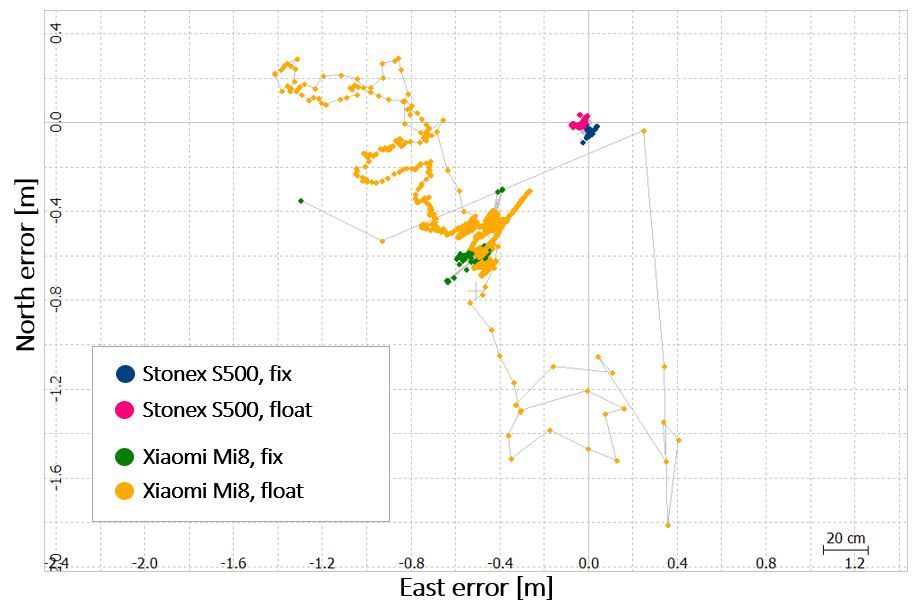
\includegraphics[width=0.48\textwidth]{fig/test4/test4_pp_scatter.jpg}} 
    \subfigure[]{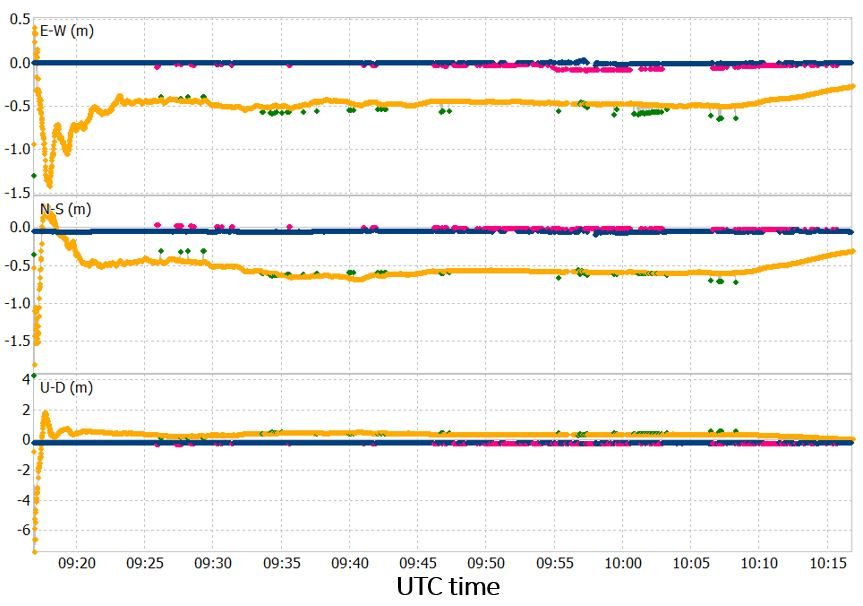
\includegraphics[width=0.48\textwidth]{fig/test4/test4_pp_timeserie.jpg}} 
    \caption{(a) Scatter plot of the positioning error for Xiaomi Mi8 and Ubox ZED F9P  (b) time series of the positioning error for Xiaomi Mi8 and Ubox ZED F9P}
    %\label{fig:foobar}
	\label{FIG:test4_pp} 
\end{figure}

The statistics values, in terms of RMS and standard deviation with respect to the precise coordinates of the receivers, are reported in Table \ref{tab:test4_pp}.

\begin{table}[H]
	\centering
	\begin{tabular}{|c|p{1.5cm}|p{1.5cm}|p{1.5cm}|p{1.5cm}|p{1.5cm}|p{1.5cm}|}
	\hline
	\textbf{Receiver} & \textbf{RMS E [m]} & \textbf{RMS N [m]} &
	\textbf{RMS H [m]} &\textbf{STD E [m]}&\textbf{STD N [m]}&\textbf{STD H [m]}\\
    \hline
	Xiaomi Mi8 & 0.499 &0.549 &0.556  &0.133 & 0.151&0.411\\  
    \hline
	Ublox ZED F9P & 0.021 & 0.043 & 0.020&0.179&0.017&0.018\\ \hline
	\end{tabular} 
	\caption{Test 4, Post processing results}
	\label{tab:test4_pp}
\end{table}

In this case study the solution for the Xiaomi Mi8 receiver has a convergence time of about 5 minutes. After this time interval the standard deviation of the solution are 0.051 m, 0.08 m, 0.093 m for East, North and Height components respectively.The solutions then presents a centimeter level accuracy, nevertheless the Ublox ZED F9P solution result more accurate. After the convergence time the Xiaomi Mi8 solution has average deviations from the precise point coordinates of -0.460m, -0.549m and 0.390m for East, North and Height components respectively. It can be state that the solution presents a decimeter precision level, but once again the Ublox ZED F9P solution results more precise.

Similarly to the previous tests the two solution can be compared in term of number of solutions and percentage of fix solution obtained. Coherently to the results already obtained for the other case studies, the Xiaomi Mi8 has a lower number of solutions (3473 against 3501) and a lower percentage of fixed solutions (2.4\% against 81.3\%).

For this case study it's also interesting to anal the solution in the time interval in which the multipath was induced, i.e. between the 9:45 and the 10:00 UTC. For the Ublox ZED F9P the solution results particularly degraded (see Fig. \ref{FIG:test4_pp}b), and almost the totality of the float solutions obtained for this receiver is in this time interval. Concerning the Xiaomi receiver the solution doesn't seem particularly degraded in this time interval with respect of the entire test period, nevertheless in this interval some false fixed solution can be observed. 

In this chapter an assessment of the quality of the GNSS position from a smartphone receiver is performed. For this purpose many tests were performed under different boundary condition and using different processing techniques, in this chapter the 4 most significant tests were reported and commented. Summarising the obtained results it's possible to state that on average the quality of the satellite signal received for smartphone receiver is definitely lower with respect to both geodetic GNSS receiver (e.g. GENU receiver in test one), but also to mass market GNSS receiver (e.g. Ublox ZED F9P in test 4). This is due to the low quality of the smartphone hardware, in particular of the antenna which is not designed for GNSS positioning. Concerning Stand Alone positioning typical accuracy and precision obtained from a smartphone are in the order of few meters. Concerning post processing relative positioning, the accuracy and precision are in the order of decimeters in both static and kinematic situations. It can be also state that in post processing approach the phase ambiguity can be hardly fixed with smartphone's observables. Furthermore the fix solution obtained are often false fixed. These false fixed solutions together with other outliers definitely compromise the robustness of the GNSS positioning by smartphone. 
\chapter[An approach to increase robustness in GNSS positionings]{\centering \begin{normalsize} \begin{Huge}
		An approach to increase robustness  in GNSS positioning
		\end{Huge} \end{normalsize}}
\label{ch:service_devel}

%\section{Workflow description}
%\section{GNSS raw: app for recording GNSS data from Android devices and sending them to a server}
%\section{Development of a low-cost permanent station for RTK positioning}

The GNSS positioning performances from smartphone devices is deeply exposed in chapter \ref{ch:quality_analisys}. The accuracy and precision obtainable in a relative post processing positioning are in the order of decimeters. Similar results can also be  obtained in real time, performing a RTK positioning. But, as highlighted by the tests performed, GNSS positioning from smartphones suffers from false fixed solutions, and outliers that compromise the robustness of the positioning itself. Those false fixed solution can be caused by many factors including the poor quality of the GNSS observables and the presence of external interferences such as multipath.
In this chapter, we present a solution to increase the robustness of GNSS RTK positioning using an Android device as a rover, and a low cost GNSS receiver as a base station. More in detail, in this chapter explains the architecture proposed highlighting the endpoints peculiarities and infrastructure realised from the communication between them. In the last part of the chapter particular attention is posed to the strategy implemented for increasing the robustness of the solution by means of the mitigation of the multipath error.
%
%\section{GNSS RTK positioning with Android devices}
The architecture of the GNSS RTK positioning procedure that we used to process GNSS data coming from Android smartphones consists of the following components:
\begin{itemize}
\item A smartphone for data acquisition;
\item A GNSS base station; 
\item A remote server for RTK processing.
\end{itemize}
The smartphone is supposed to be equipped with an Android App capable of reading GNSS raw observables, packing them in a proper way, and send them to a server running RTKLIB through a TCP socket. The base station must be capable of sending in real time it's observables together with it's precise coordinates to the server. The server is supposed to be capable of reading the input streams from the smartphone and from the base station, processing them with RTKLIB, and then returning the coordinates to the smartphone. 
The resulting architecture is shown in figure \ref{FIG:dev_rtk_arch}.
\begin{figure}[H] 
	\centering
	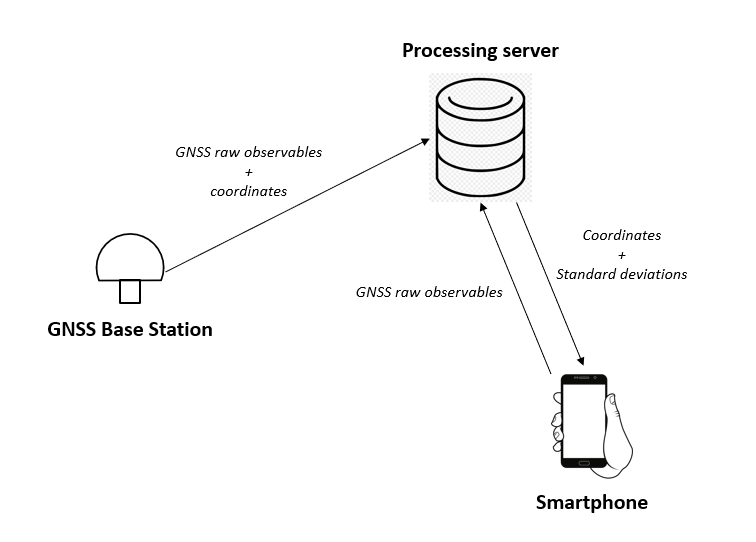
\includegraphics[scale=0.80]{fig/dev_rtk_arch.PNG} 
	\caption{Proposed architecture for robust RTK positioning with smartphone}
	\label{FIG:dev_rtk_arch} 
\end{figure}
The proposed system works with an ah-hoc GNSS base station assembled with a low cost GNSS receiver, but can be generalised by using an NRTK network instead. In the following sections the implementation of the different components are described in detail.
\section{GNSS base station}
\label{par:lige}
The first element of the developed architecture for GNSS RTK positioning with Android smartphones, is the GNSS base station. This paragraph describes the GNSS base station built, using a low cost hardware, and the software written for data acquisition and delivery. 
The hardware  is based on the dual frequency and multiconstellation GNSS receiver ublox ZED F9P. The performance of this receiver have been investigated in literature in many application \cite{Wielgocka:2021, Nguyen:2021,Hohensinn:2021}, and in open sky environment it can be considered a valuable alternative to geodetic-grade GNSS receivers \cite{janos:2021}. The GNSS receiver is coupled with the Hemisphere A45 antenna mounted in the rooftop of Gter's office, in Genoa. The base station hardware (see fig \ref{FIG:ligehw}) is completed with a Raspberry Pi used for data logging and delivery.
%
\begin{figure}[H] 
	\centering
	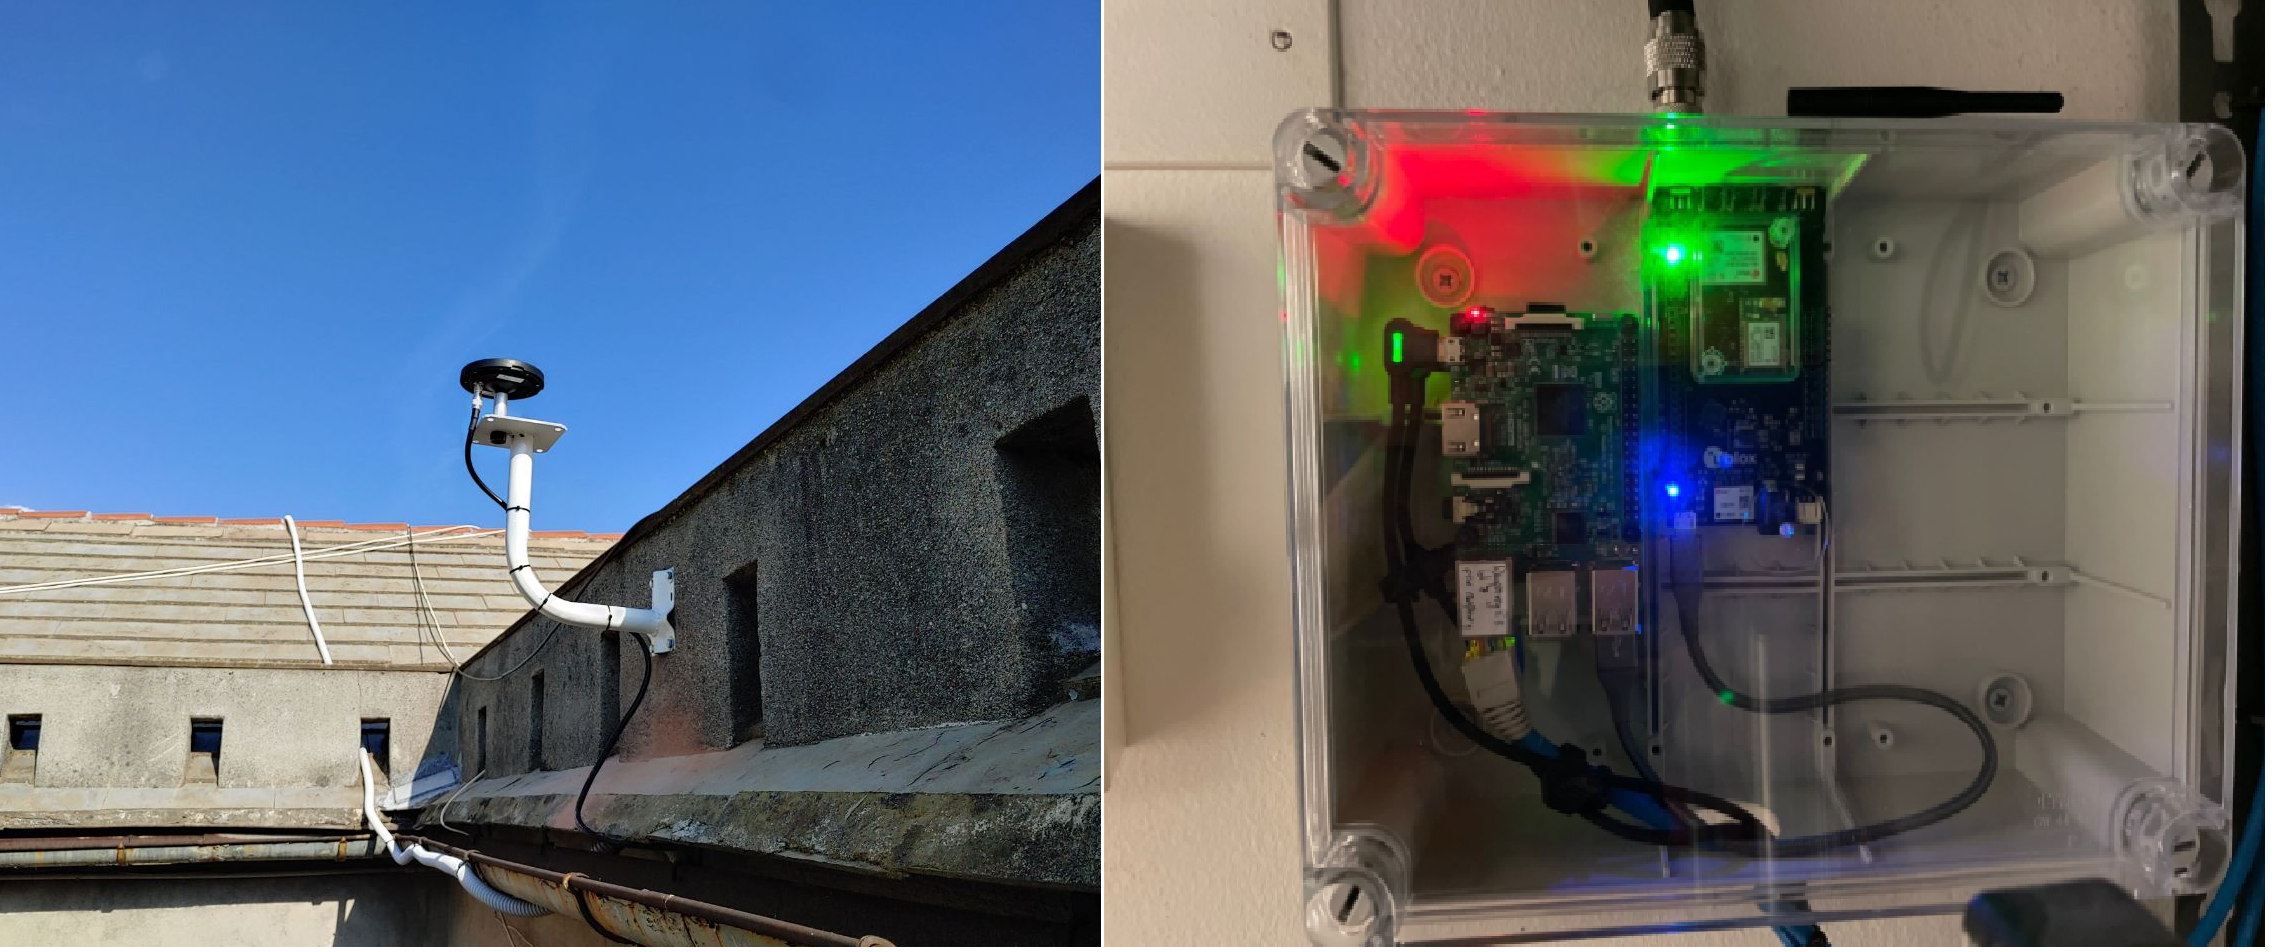
\includegraphics[scale=0.40]{fig/gnss_base_lige.png} 
	\caption{GNSS base station hardware}
	\label{FIG:ligehw} 
\end{figure}
%
The main functions of the GNSS station are:
\begin{itemize}
\item Publish the GNSS raw measurement stream  to users in real time over the Internet;
\item Recording hourly RINEX files and publish them on a ftp server.
\end{itemize}
%
In order to fulfil these two functions, the RTKLIB software was installed in the Raspberry Pi, and a few Python scripts were developed for background management of the processes. Figure \ref{FIG:ligesw} shows the developed software architecture.

\begin{figure}[H] 
	\centering
	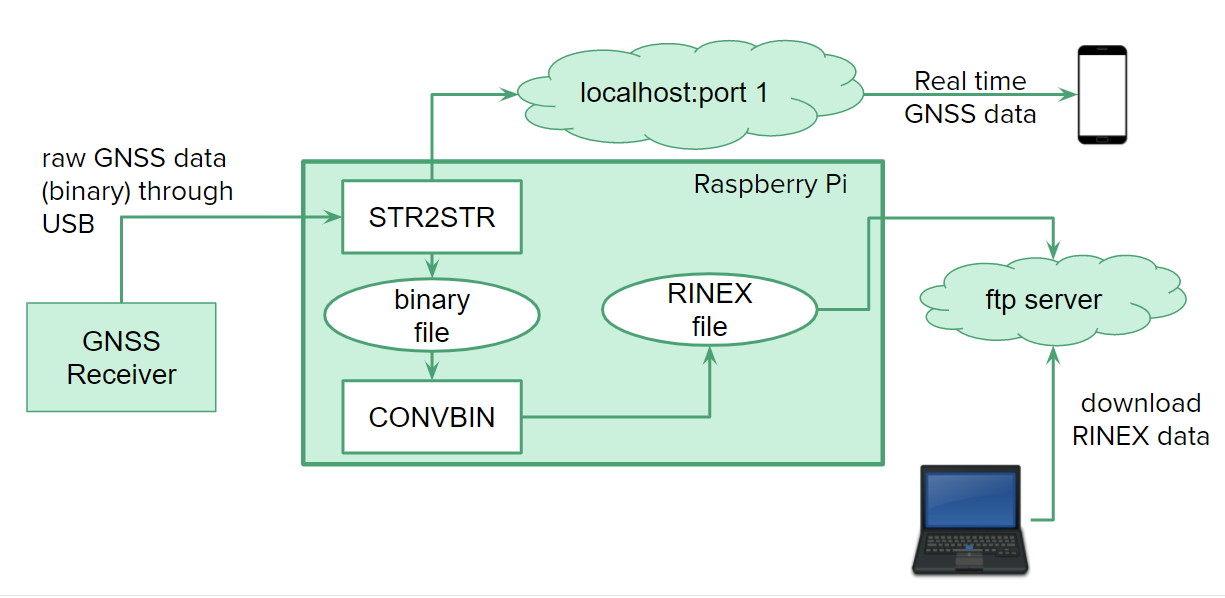
\includegraphics[scale=0.60]{fig/lige_sw_architecture.PNG} 
	\caption{GNSS base station software architecture}
	\label{FIG:ligesw} 
\end{figure}

In this GNSS base station the receiver is connected to the Raspberry Pi via USB, so the GNSS raw measurement observed by the receiver, must be transmitted to the Raspberry Pi through this channel.
By default the ublox GNSS receiver doesn't include the GNSS raw measurement in their stream coming out of the USB, but they have to be included manually. This operation can be done using the ublox management software u-center\footnote{\url{https://www.u-blox.com/en/product/u-center}}. Under the configuration menu, there's the possibility to include different messages to the output stream of the GNSS receiver. For having GNSS raw measurement in the USB output stream the messages to include are the ``RXM-RAWX", and the ``RXM-SRFBX". Once these messages are included, the GNSS receiver can properly work with RTKLIB modules. Another important option that can be set before using the GNSS receiver with RTKLIB is the acquisition rate. For this application the acquisition rate is set equal to 1Hz.

As shown in fig. \ref{FIG:ligesw}, the first block in the chain is the RTKLIB module STR2STR. This module is able to read an input stream and redirect it through different channels. In this case the input stream comes from the USB port, and it's redirected to a TCP port and to a file. The stream through the TCP port can be access by external user in order to perform a GNSS RTK positioning. The other output stream is saved to a file. This file is in binary format (ubx) so in order to be used for post processing application it shall be converted into RINEX format. This conversion can be done with the RTKLIB module CONVBIN. 
Process management is delegated to a couple of Python scripts: \textit{start\_acquisition} and \textit{stop\_and\_upload}. The first scripts simply launches an instance of STR2STR and saves in a temporary file the STR2STR's PID (Process ID), the path and the name of the local file created. When executed, the  \textit{stop\_and\_upload} script reads the information form the temporary file, kills the STR2STR and launches the CONVBIN software for RINEX conversion. Once the conversion is terminated, thanks to the Python's library \textit{ftplib} the RINEX file is upload to a ftp server and made available to users.
Properly inserted into \textit{"/etc/crontab"} file (i.e. the file that manages the automatic execution of software and scripts in a Raspberry Pi or more in general in a UNIX system) this two scripts allow having a continuous stream of GNSS raw observable through a TCP port and hourly RINEX file published in an FTP server. 
The code developed is also made available in the Gter's GitHub page\footnote{\url{https://github.com/gtergeomatica/GNSSBase_station_ublox}}.

\section{Android Application}
\label{sec:gnssraw}
%
The second component of the architecture  is a smartphone capable of accessing GNSS raw measurement. In order to make the smartphone working in this architecture, a specific Android App, named  ``GNSS Raw", is conceived and developed. The purpose of this app is to read data from the Android device in which it is installed, sending them to a remote server, and reading and plotting the position computed by the server with those data.
The application is written in Java and it is compatible with all devices running an Android version higher than 7.0 Nougat. During the PhD work we have developed two versions of the App. More specifically, in the second release we have improved data preparation and added services to visualise the computed position, run the app in background, and disable duty cycle directly in the app (for Full Track surveys) without the need to disable it from the developer options menu. This last feature is available only for devices having Android version higher than 12 (API level 31).

The application, based on the GNSS Logger app released by Google\footnote{\url{https://github.com/google/gps-measurement-tools/tree/master/GNSSLogger}} is composed by 5 different menu:
\begin{itemize}
\item Measurement
\item Plot
\item Map
\item Files
\item Settings
\end{itemize}
In the rest of the section we will describe each functionality while focusing on important points in 
the implementation of the Java code.
%
\subsubsection*{Measurement}
The Measurement menu presents a very simple GUI (Graphical User Interface) as shown in figure \ref{FIG:gnssraw_measurement}, and is used to to start and stop data recording.
\begin{figure}[H] 
	\centering
	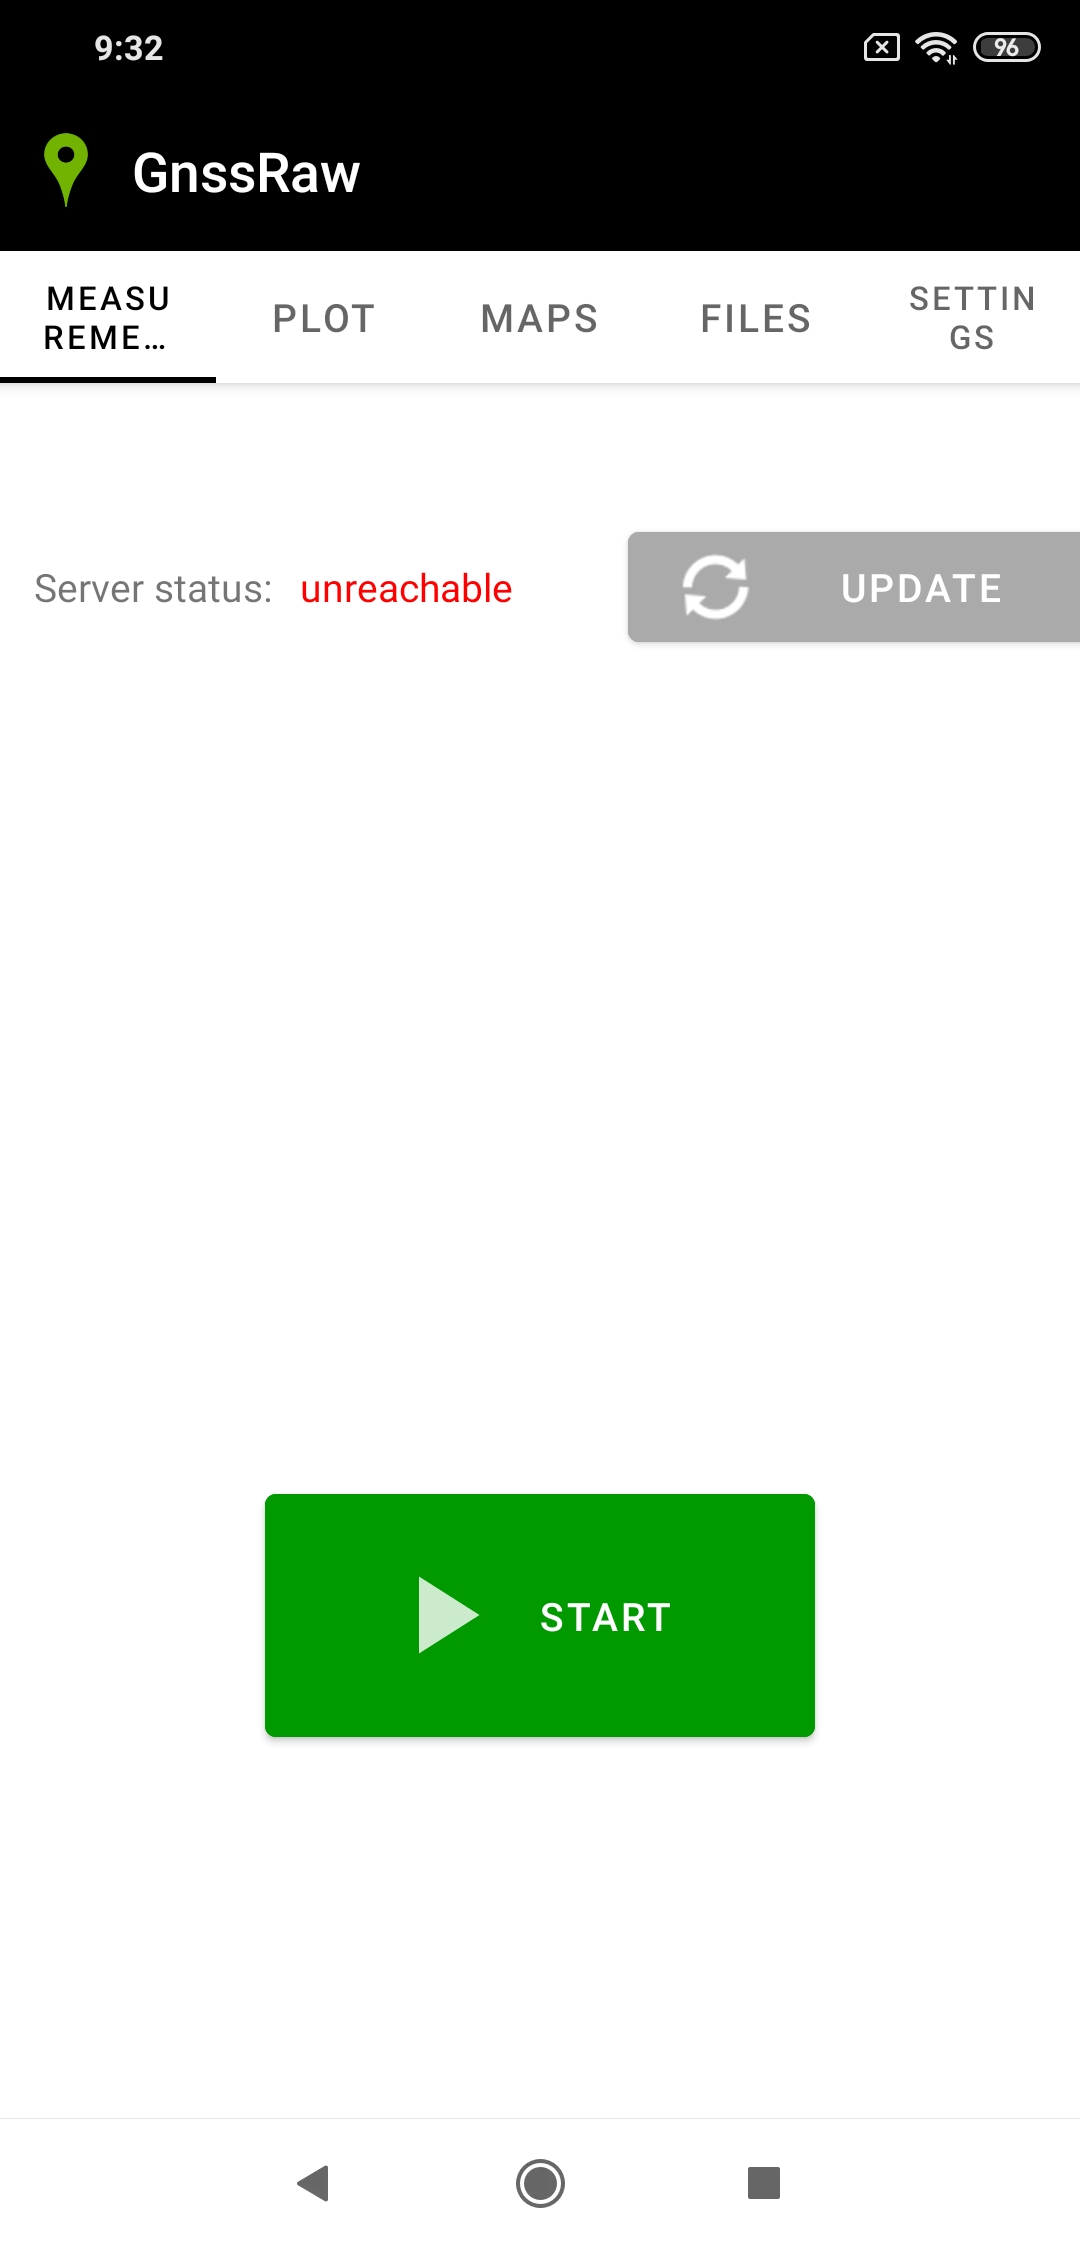
\includegraphics[scale=0.15,frame]{fig/gnssraw_measurement.jpg} 
	\caption{GNSS Raw: Measurement menu}
	\label{FIG:gnssraw_measurement} 
\end{figure}
When the start button is pushed, the GNSS raw measurement data (see chapter \ref{ch:SoA}) are saved in a local file and sent to a remote server (when reachable) in real time. 
The procedure for accessing the GNSS raw data from the smartphone GPS receiver are described next.
\subsubsection*{Data Acquisition}
The Java code that implements data acquisition, processing and communication is listed in Appendix \ref{appendix:androidcode}
organized in accord with the class diagram depicted in Fig. \ref{FIG:class_diagram}. 
\begin{figure}[H] 
	\centering
	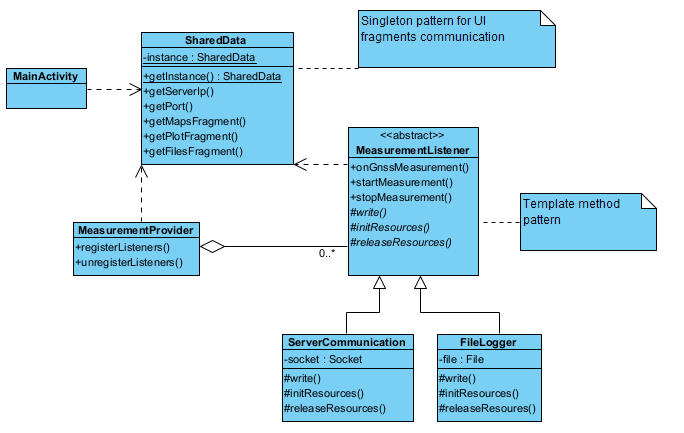
\includegraphics[scale=0.80,frame]{fig/class.png} 
	\caption{Class diagram}
	\label{FIG:class_diagram} 
\end{figure}
More specifically, we defined the following Java classes:
\begin{itemize}
\item 
the class \verb+MeasurementProvider+ that contains the software configuration of the GNSS engine (e.g. managers, listeneres, and sampling intervals);
\item 
the class  \verb+MeasurementListener+ that specifies the  data collection listeners;
\item 
the class \verb+ServerCommunication+ (that extends 
\verb+MeasurementListener+) that provides the API communication layer between the smartphone and the RTKLIB server.
\item 
the singleton class \verb+SharedData+ is used to encapsulate all data used in the application, to share data among different tabs, 
and to decouple the application logic from its view component (the fragments used in the UI).
\end{itemize}
The \verb+MeasurementProvider+ class creates a \verb+LocationManager+ object and the callbacks and parameters used for setting up the GNSS data acquisition.  
The \verb+LocationManager+ class provides access to the system location services, and in particular allows applications to obtain periodic updates of the device's geographical location. Starting from API level 24, using this class it's also possible to access GNSS raw measurements. In order to get those data a specific callback has been created.\footnotemark{A callback is a function  that is passed into another function as an argument and is expected to execute after some specific type of event.} The callback is invoked every time  a new measurement occurs and it is used for receiving GNSS satellite data. Each measurement contains raw and computed data identifying a satellite. 
The sampling rates are defined via the static attributes \verb+LOCATION_RATE_GPS_MS+ (1 second) 
and \verb+LOCATION_RATE_NETWORK_MS+ (1 minute).

The public method \verb+onGnssMeasurementsReceived+, used in the above mentioned class, reports the latest collected  GNSS measurements from the GNSS engine via  listener.
The listener provides a callback to be invoked when the \verb+MeasurementManager+ updates the sensors and signals data. 
The callback invokes the  method \verb+onGnssMeasurementsReceived+ of the \verb+MeasurementListener+ class. The method invocation received  \verb+event+ object that contains the raw measurement data in the format of the Android GNSS raw data library.
To correctly process those measurements, it's necessary to send to the RTKLIB server all the measurements referred to the same epoch in an unique block. For this reason, the implemented callback checks the epoch of every measurement and creates an unique string with all the measurement referred to the same epoch. This string is sent to the server in order to be processed.

More specifically, the method \verb+onGnssMeasurementsReceived+ computes the current timestamp using the \verb+getClock()+ method of the corresponding event. Every satellite measurement shares the same clock value up to milliseconds. The milliseconds timestamp of each single piece of data can be extracted from the event object via the \verb+event.getMeasurements()+ method. 
Data of the different satellites are then packaged into a single string delimited by two special sentinels ("NB" and "FB") via 
by invoking  the method \verb+getMeasurementInfo+.
The packaging phase is executed in the body of the listener 
(not on separate threads) since it does not seem to affect the performance of the app.   
%
\subsubsection*{Data Transmission}
%
In order to set up the Client-Server communication simple TCP sockets from the standard Java network library (java.net) were used.
To correctly set up the communication with the server, the server's IP and the port, must be specified in the relatives boxes (figure \ref{FIG:gnssraw_settings}. The reachability status of the server can be checked by the user in the "Measurement" menu.
The communication is active by default, but the application gives also the possibility to turn it off. In this case the application doesn't perform any positioning, but simply records GNSS raw data. 
Assuming the server is reachable, the app sends the packaged GNSS raw measurements to the server using the \verb+write+ method of the  \verb+ServerCommunication+ class.
Differently from the data preparation phase, 
the \verb+ServerCommunication+ class employs a thread pool in order to schedule data transmission on a dedicated thread to avoid to block the UI in case of transmission delays.
%
\subsubsection*{Plot}
The Plot menu (figure \ref{FIG:gnssraw_plot}) is activated only when the start button is pushed. Similarly to the Google GNSS logger app, this menu, shows the $SNR$ trend over time. This parameter is a good indicator of the quality of the incoming signal, and it's useful to keep it monitored during a survey in order to understand which satellites may cause problems in the positioning. The GNSS Raw app allows to filter this graph by constellation or by individual satellite.

\begin{figure}[H] 
	\centering
	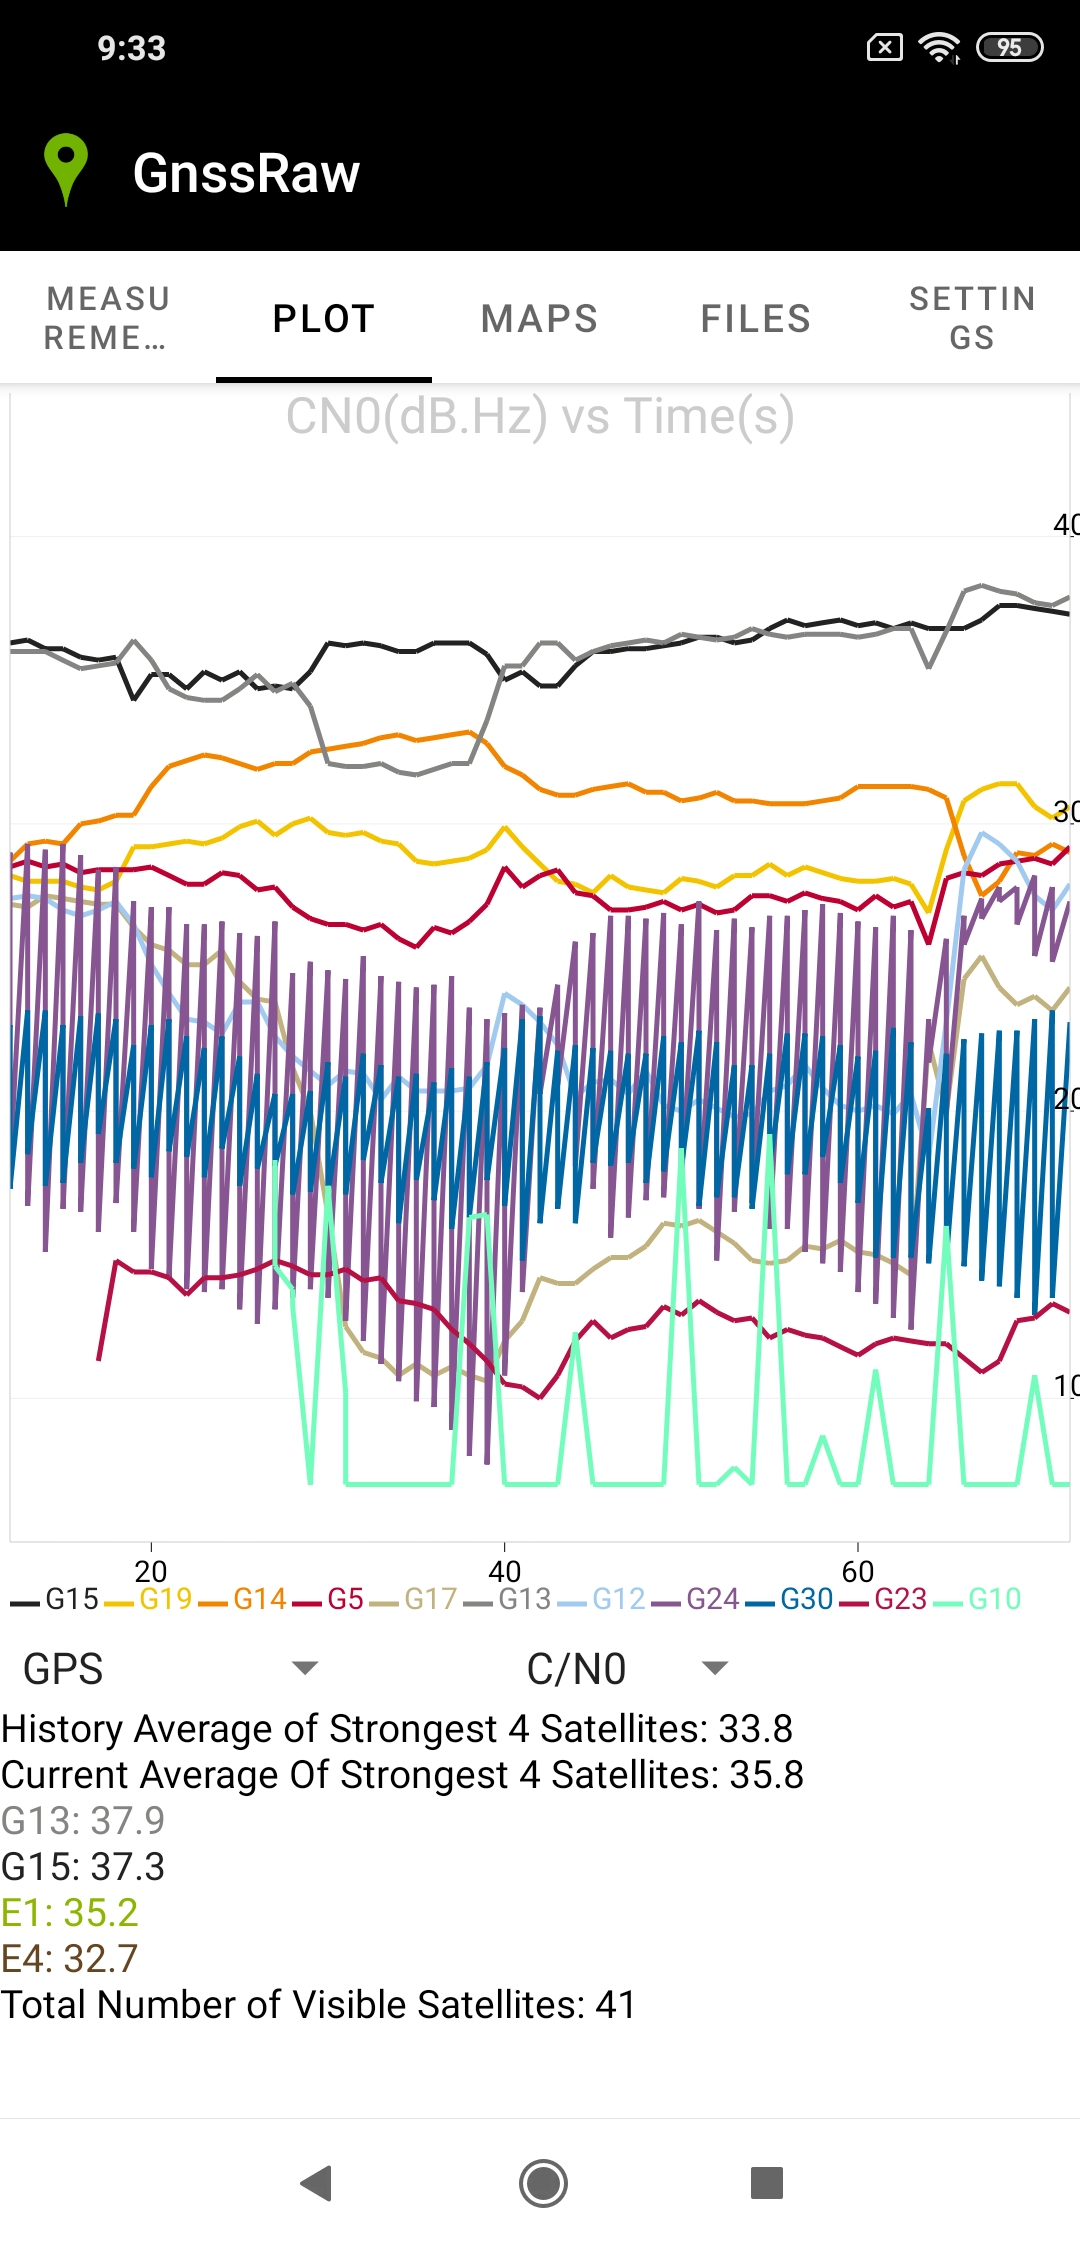
\includegraphics[scale=0.15,frame]{fig/gnssraw_plots.jpg} 
	\caption{GNSS Raw: Plot menu}
	\label{FIG:gnssraw_plot} 
\end{figure}

The GNSS raw, implements a menu for viewing the recorded files with GNSS raw measurement (figure \ref{FIG:gnssraw_file}), without using the smartphone's integrated file manager. In order to keep order between all the recorded files, the filename criteria adopts the simple rules ``GNSS\_Log" suffix followed by the date. This menu also allows user to share the recorded data through common sharing channels, and gives the possibility to eliminate them from the local storage memory. 

\begin{figure}[H] 
	\centering
	\includegraphics[scale=0.15,frame]{fig/gnssraw_files.jpg} 
	\caption{GNSS Raw: File menu}
	\label{FIG:gnssraw_file} 
\end{figure}
\subsection*{Settings}
The Settings menu (figure \ref{FIG:gnssraw_settings}) is mainly used to set up the communication between the smartphone and the remote server running RTKLIB.

\begin{figure}[H] 
	\centering
	\includegraphics[scale=0.15,frame]{fig/gnssraw_settings.jpg} 
	\caption{GNSS Raw: Settings menu}
	\label{FIG:gnssraw_settings} 
\end{figure}
\subsection*{Map}
 The results of the processing (i.e. the coordinates and the associated standard deviations) are sent to a tcp server on the same host, by means of a native RTKLIB function. The GNSS raw app connects to this server using another socket and get the processed data. Those data are than parsed and plotted in the Map menu (figure \ref{FIG:gnssraw_map}).   
The marker in the map changes color accordingly to the solution status. In particular the marker becomes green if the solution is Fix, yellow is the solution is Float and red if the solution is Stand Alone (i.e. the relative positioning couldn't be performed).

\begin{figure}[H] 
	\centering
	\includegraphics[scale=0.15,frame]{fig/gnssraw_maps.jpg} 
	\caption{GNSS Raw: Map menu}
	\label{FIG:gnssraw_map} 
\end{figure}
The source code of the app has been also translated and optimized to Kotlin language, which is now supported by Google as an official language for Android apps. The Kotlin code of the app is available on a branch of the GitHub repository of the app. \\
The GNSS raw application has been designed in order to read and send to the server not only GNSS raw data, but also data coming from the other sensor embedded in the smartphone. The main idea is to send to the server, also data coming from accelerometer, gyroscope and magnetometer, to investigate the possibility to perform server side, an integration between GNSS and INS data from smartphone. This kind of integration is not object of this work and the function to record data from other sensor in the smartphone is still under development.
%
\section{RTKLIB Server}
\label{sec:modified_rtklib}
The last component of the architecture is a remote server for GNSS positioning. The server should have installed an RTKLIB version for data processing and should be able to communicate in real time with both the smartphone and the Base station though tcp sockets. In the specific case an Ubuntu 20.04 server has been chosen. Concerning the GNSS processing, the standard version of RTKLIB only few formats for input GNSS data, including the standard ones (RTCM 3, RTCM2 and BINEX) and some GNSS manufacturers proper binary format. The original version of RTKLIB is not capable of working in real time with GNSS data coming from Android devices, as the format in which they are accessed is not recognised by the software. The ``Android format" is the one generated by the ``GNSS raw" app (see par \ref{sec:gnssraw}). In order to overcome this issue, in the ambit of this work, the original version of RTKLIB was modified, in order to perform, a RTK GNSS positioning using data coming from an Android smartphone.  This section explains in details the software modification done to make RTKLIB compatible with Android format. In rtksvr.c there's the \textit{decoderaw} function used to decode input data and saving them in the proper structure to be elaborated. The \textit{decoderaw} function has 3 different cases depending on input data format, and for each cases implements the following function:
\begin{itemize}
\item \textit{input\_rtcm2} for decoding RTCM v.2 data
\item \textit{input\_rtcm3} for decoding RTCM v.3 data
\item \textit{input\_raw} for decoding binary data from the supported receivers
\end{itemize}

Differently from \textit{input\_rtcm2} and \textit{input\_rtcm3} functions, the \textit{input\_raw} requires as an argument, in addition to the data to be decoded, the format of that data. This parameter must be specified by the user in the configuration file. For every supported format RTKLIB implements a different decoding function. The main RTKLIB modification consists in the generation of a new format together with it's relative decoding function, called \textit{decode\_gterAndroid} used to decode the data sent from the ``GNSS raw" app (see par. \ref{sec:gnssraw}). Before entering this function, an entire block of data must be recognised from the input stream. This operation allows to pass to the \textit{decode\_gterAndroid} function a set of observables all referring to the same epoch, which is essential for the rest of the processing. Data recognition is based on the fact that each block of data referred to the same epoch, is packed in a specific way, and has an identification character needed for its synchronisation. After a block of data is recognized the \textit{decode\_gterAndroid} function is executed.
The first operation performed by the function is to recognise and isolate within the block of data read the subsets of observables corresponding to each single satellite. Then, for each set of observables, using the strategies described in chapter \ref{ch:SoA}, the following parameters are calculated:
\begin{itemize}
\item Satellite ID
\item Frequency and observation code
\item GPS week and GPS second of week
\item Pseudorange
\item Carrier phase 
\item Doppler
\item Signal to Noise Ratio
\end{itemize}
Once they have been computed, the quantities are saved in the proper RTKLIB structure in order to be used in the part of the software workflow. In the pseudo-range and carrier phase computation some controls are implemented as suggested in \cite{GSA_wp:2016}. In particular for the pseudo-range computation it is necessary to control the decoding status of the Time Of Week (TOW) value, an essential parameter for the correct generation of pseudo-range. 
In other words even a small uncertainty on the TOW could lead to a completely wrong value of the pseudo-range which in turn could significantly degrade the quality of the final positioning. The decoding status of the TOW can be retrieved using the GNSS Android API. By comparing this value with some defined constants (see table \ref{tab:api_constants}), it is possible to distinguish whether the TOW is properly decoded or not. In case the TOW results not properly decoded the pseudo-range it is not computed.

Concerning the carrier phase generation, a check is made on the validity status of the observable. In this case the GNSS 
Android API presents a specific field, called \textit{AccumulatedDeltaRangeState}, used for this purpose. Furthermore this field is also used to verify the presence of cycle slips. Considering the high noisiness of GNSS observables from smartphones a second check is implemented on carrier phase generation. This second check is performed using the field \textit{AccumulatedDeltaRangeUncertaintyMeters} that provides and estimation of the uncertainty in meters on the accumulated delta range quantity. In the modified RTKLIB version a new configuration parameter, called \textit{maxadru} was introduced, to discard all the carrier phase measurements whose \textit{AccumulatedDeltaRangeUncertaintyMeters} parameter is higher than the specified value. By default the \textit{maxadru} parameter is equal to 0.1 meters.
%
\section{Multipath Mitigation Heuristics}
One of the major external interference that degrade GNSS 
positioning is multipath. The effect of this interference is well described by its name: a satellite-emitted signal arrives at the
receiver from different directions (i.e following different paths). Multipath effect is mainly caused by reflecting surfaces
nearby the receiver. For this reason, it frequently happens  in urban canyons, a typical scenario in which smartphone are used.
Multipath effect may also occur when using low cost GNSS receivers equipped with low quality antennas, such as the smartphone's ones. For this reason a good strategy to improve the robustness in GNSS positioning from Android devices should aim at mitigating the multipath error. 

Multipath mitigation can be performed at the Antenna, Receiver (Signal Processing) and Navigation Solution Level \cite{Bhuiyan:2010}. 

%Concerning antenna level mitigation possible solutions are 

In this work the multipath mitigation is attacked at software level, using an algorithm, called MDP (Multipath Detection Parameter) conceived by Gter. In the following section the algorithm is explained in detail together with its implementation in RTKLIB.
\subsection{The MDP Algorithm}
The MDP algorithm consists in two main parts: the first one concerning multipath detection, and the second one concerning multipath mitigation.
The multipath detection part is based on the SNR (Signal to Noise Ration) value and a new variable called MDP (Multipath Detection Parameter). The aim of the MDP value is to create a variable representative for multipath effect for single frequency GNSS receivers, starting from the observation equation. 
The observation equations for GNSS are:
\begin{equation}
    \begin{matrix}
        P(t_{1})=\rho(t_{1})+\Delta T_{r}^{s}(t_{1}) + Ion(t_{1}) + Trop(t_{1}) + Mult(t_{1}) + \epsilon \\
        L(t_{1})=\rho(t_{1})+\Delta T_{r}^{s}(t_{1}) - Ion(t_{1}) + Trop(t_{1}) + mult(t_{1}) + \lambda N+ \epsilon
    \end{matrix}
\label{eq:obs_multipath}
\end{equation}
where
\begin{itemize}
\item \textit{P(t\textsubscript{1})} is the pseudorange observable at instant \textit{t\textsubscript{1}}
\item \textit{L(t\textsubscript{1})} is the carrier phase observable at instant \textit{t\textsubscript{1}}
\item $\rho(t_{1})$ is the geometric range between the satellite and the receiver at instant \textit{t\textsubscript{1}}
\item $\Delta T_{r}^{s}(t_{1})$ is the global time unknown at instant \textit{t\textsubscript{1}}
\item $Ion(t_{1})$ is the ionospheric effect on the signal at instant \textit{t\textsubscript{1}}
\item $Trop(t_{1})$ is the tropospheric effect on the signal at instant \textit{t\textsubscript{1}}
\item $\lambda N$ is the phase ambiguity
\item $Mult(t_{1})$ is the code multipath
\item $mult(t_{1})$ is the phase multipath
\item $\epsilon$ represents residual errors due to noise.
\end{itemize}

The reported equations are valid for GPS and Galileo. If GLONASS constellation is considered, then the inter-channel bias should also be added to the model.

One common approach to isolate the multipath effect from equations \ref{eq:obs_multipath} is to compute their difference \cite{Bisnath:2001}. The result is the so-called sentinel variable:
\begin{equation}
    S(t_{1}) = P(t_{1})-L(t_{1}) = 2Ion(t_{1})- \lambda N + (Mult(t_{1}) - mult(t_{1}))
\label{eq_sentinel}
\end{equation}
The definition of MDP variable requires two assumptions. 
Considering a sufficiently high acquisition rate (i.e. 1 Hz), we can 
assume that:
\begin{itemize}
    \item The ionosphere effect is equal between 2 consecutive epochs;
    \item The phase ambiguity is equal between 2 consecutive epochs.
\end{itemize}
Based on these assumptions, the MDP variable is defined as:
\begin{equation}
    MDP=S(t_{2})-S(t_{1})=\{ [Mult(t_{2})-mult(t_{2})]-[Mult(t_{1})-mult(t_{1})]\}+\epsilon
\label{eq:mdpvariable}
\end{equation}
Hence, as shown in equation \ref{eq:mdpvariable}, the MDP variable is representative of the effect of multipath effect and   
residual errors due to noise.
\subsubsection{MDP: Detection Algorithm}
The detection algorithm compares the SNR and  MDP parameters to
static and dynamic threshold values as explained below.
\paragraph*{SNR Threshold} The multipath detection part proposed in the MDP algorithm exploits also the SNR value, which is not a specific indicator for multipath but for noise in general. The aim of checking also the SNR mask is to identify outliers which can be caused by multipath, other external interference, or can refer to corrupted data.
More specifically, for the SNR parameter 
a static threshold is set before running the positioning procedure. The value to be assigned to the SNR threshold depends on several factors, such as the quality of the GNSS antenna and the environmental conditions of the survey. The optimal value to assign to the threshold is still object of research. In this work, it is determined experimentally by trying different configurations, as explained in the chapter \ref{ch:mdp_results}.
Epoch by epoch for each acquired observable the SNR value is compared to the chosen threshold: if the SNR value is lower than the threshold, the observable is flagged with a so-called SNR flag.
\paragraph*{MDP Threshold}
The MDP is a parameter specifically designed to identify data affected by multipath. Under normal conditions, i.e. absence of multipath, the variable MDP is expected to have a white noise trend, and it's values depend on the entity of residual errors due to noise. In case of incoming multipath, the MDP variable is expected to have some outliers. The aim of the MDP threshold than is to identify those outliers, as they indicate multipath affected data. Two difference MDP thresholds were introduced in this work: a static one and a dynamic one. The static MDP threshold is used in a similar way to the SNR threshold. The optimal MDP threshold value is still object of research and in this work, it is determined experimentally by trying different configurations, as discussed in the chapter \ref{ch:mdp_results}.  Once the MDP static threshold is set, epoch by epoch for each acquired observable the MDP value is computed and compared to the threshold. The observable is then flagged with a so-called MDP flag if:
\begin{equation}
|MDP| \geq mdpthreshold 
\label{eq:mdpthres}
\end{equation}
Concerning the MDP, also an adaptive threshold was proposed. This adaptive threshold is computed considering a statistical analysis on previous epochs. 
The heuristics is based on an additional parameter, $N$, that defined the length of the observation window (number of epochs to be analysed). As the aim of the MDP threshold is to detect outliers, the Chebyshev's inequality is used for its definition. In fact, Chebyshev’s inequality states that, considering a broad range of probability distributions, 88.89\% of values lies within three standard deviations of the mean \cite{chebyshev:1}. The MDP adaptive threshold is then defined as:
\begin{equation}
mdpthreshold = \mu \pm 3\sigma
\label{eq:mdpthres_din}
\end{equation}
where
\begin{itemize}
    \item $\mu$ is the mean MDP value on $N$ previous epochs;
    \item $\sigma$ is the standard deviation of the $N$ previous MDP values;
\end{itemize}
In this case the observable is flagged if:
\begin{equation}
MDP \leq \mu -3\sigma \vee MDP \geq \mu + 3\sigma
\label{eq:mdpthres_dyn}
\end{equation}
\paragraph*{Initialization Phase}
The detection part of the algorithm when the MDP dynamic threshold is chosen, needs an initialization time equal to $N$ times the acquisition rate. Therefore, for example, if the acquisition rate is 1Hz and $N$ is equal to 60, the detection algorithm needs 1 minute to reach a complete operating status. 
\paragraph*{Detection Phase}
Based on the current values of the MDP and SNR flags, the detection algorithm implements 3 different criteria to state if the observable is affected by multipath. Those criteria are:
\begin{itemize}
    \item Crit 1.: Only MDP flag
    \item Crit 2.: MDP flag and SNR flag
    \item Crit 3.: MDP flag or SNR flag
\end{itemize}
Figure \ref{FIG:mdp_workflow} summarises the resulting detection algorithm.
\begin{figure}[H] 
	\centering
	\includegraphics[scale=1]{fig/mdpscheme.png} 
	\caption{MDP: Detection part of the algorithm}
	\label{FIG:mdp_workflow} 
\end{figure}
\clearpage
For each epoch, using this procedure, a set of observables potentially affected by multipath is identified. 
The detection phase is used then to trigger the mitigation procedure.
\subsubsection{MDP: Mitigation Algorithm}
The aim of the mitigation algorithm is to retrieve a more accurate and precise GNSS positioning taking into account multipath-affected observables. One possible way to mitigate multipath effect is to exclude the multipath affected observables. This heuristics runs into the risk of excluding too many GNSS observables, hence producing a poor quality result due to missing redundancies in the 
observables. In order to avoid this scenario, a good way to proceed is to consider associated different weights to the multipath-affected GNSS observables. 

Since the MDP is integrated in RTKLIB, the new proposed weight to be associated with the multipath affected observables is based on the weight that the software associates with the observables.
As previously described RTKLIB uses a weight matrix defined as:
\begin{equation}
\textbf{W}=diag\left(\sigma_{1}^{-2}, \sigma_{2}^{-2}, ...,\sigma_{n}^{-2}\right)
\label{eq:rtklib_weight_matrix}
\end{equation}
In eq. \ref{eq:rtklib_weight_matrix}, $\sigma_{n}^{2}$ is the variance associated to the n\textsuperscript{th} observable defined as:
\begin{equation}
\sigma_{meas}^{2}=F^{s}R_{r}\left(a_{\sigma}^{2}+\frac{b_{\sigma}^{2}}{sinEL_{r}^{s}}\right)
\label{eq:rtklib_weight_matrix1}
\end{equation}
where:
\begin{itemize}
    \item $F^{s}$ is the satellite system error factor which is equal to 1 for GPS, Galileo, QZSS and BeiDou, equal to 1.5 for BEIDOU and equal to 3 for GLONASS
    \item $R_{r}$ is the code/carrier‐phase error ratio
    \item $a_{\sigma}, b_{\sigma}$ are the carrier‐phase error factor a and b in meters
\end{itemize}
    
Furthermore the software adds to this variance other contributions, so the final equation becomes:

\begin{equation}
\sigma_{obs}^2= \sigma_{meas}^2+\sigma_{eph}^{2}+\sigma_{ion}^{2}+\sigma_{trop}^{2}+\sigma_{bias}^{2}
\label{eq:rtklib_variance_matrix1}
\end{equation}

where
\begin{itemize}
    \item $\sigma_{eph}$ is the standard deviation of ephemeris and clock error in meters
    \item $\sigma_{ion}$ is the standard deviation of ionosphere correction model error in meters
    \item $\sigma_{trop}$ is the standard deviation of troposphere correction model error in meters
    \item $\sigma_{bias}$ is the standard deviation of code bias error in meters [m]
\end{itemize}


In order to take into account of the multipath effect, the variance of the observables identified as potentially affected by multipath, is incremented adding a new component. This component, is based on the sigma-$\epsilon$ model \cite{Brunner:1999,Wieser:2000} used to weight GNSS observables by means of their SNR value. A new term has been added to this model in order to take into account also the multipath effect by means of the MDP value. The resulting term, called \textit{mdp variance}, is expressed by:

\begin{equation}
\sigma_{mdp}^{2}= mdp^{2}+C\cdot 10^{-\frac{SNR}{10}}
\label{eq:rtklib_mdp_variance}
\end{equation}

Where $C$ is a model parameter equal to 0.244 m\textsuperscript{2}DB-Hz for L1 frequency.
The proposed weight model is defined in a such way to amplify the impact of the multipath effect (MDP variable) with respect to external noise (SNR). 
 Since the weight associated to the observables is equal to the inverse of its variance (see eq. \ref{eq:rtklib_weight_matrix}), the weight of the observable decrease as its MDP value increase. Furthermore using the proposed MDP variance, the multipath affected observable are weighted in a different way depending on their MDP values: observables affected by a large multipath error (high MDP value) will have a lower weight with respect to observables having a lower multipath error (i.e. lower MDP value). Furthermore the MDP variance takes into account also the SNR value. As the SNR value decreases (i.e. the observable noise increases), the MDP variance associated to the variable increases and consequently its weight decreases.
%l'approccio proposto verrà validato sperimentalmente

An experimental validation of the proposed algorithm will be presented in the next chapter.
%nel prossimo capitolo verrà presentata una validazione sperimentale dell'algoritmo proposto... 

\chapter[Results analysis]{\centering \begin{normalsize} \begin{Huge}
		Results analysis
		\end{Huge} \end{normalsize}}
\label{ch:mdp_results}

In this chapter, the effects on the GNSS positioning from smartphones introduced by the application of the MDP algorithm are discussed. In particular the performance of the algorithm, in terms of multipath detection and mitigation, by varying its configuration parameters are exposed. For this purpose both static and kinematic datasets are analysed. 

\section{Processing strategy}

The datasets analysed for the evaluation of the performance of the proposed algorithm are the case studies 3 and 4 reported in chapter \ref{ch:quality_analisys}. The selected case studies are used to test the main features of the proposed architecture. They are both processed using the LIGE base station, developed for this work. They  require the use of our Android app installed on a device and the modified RTKLIB version for data processing. Although the proposed architecture has been designed for real-time applications, in order to evaluate the performance of the MDP algorithm, several post processing elaborations were computed all having the same input data, hence  under  the same contextual conditions.

%TIZIANO: non ricordo se c'è un altra sezione della tesi in cui i valori di soglia e i criteri con cui è stato creato l'MDP sono dettagliati meglio.

The MDP algorithm present several input parameters to tune the computation phase. First of all, in the detection step one out of three criterion must be selected. Moreover, the strategy for the MDP threshold computation must be chosen between the static and the adaptive one. The value chosen as static threshold remains constant for the entire computation. For the adaptive threshold value, the number of previous epochs should be set. The MDP threshold will depend then on a  statistical analysis computed on the previous MDP values following the equation \ref{eq:mdpthres_dyn}.  Finally the SNR threshold must be set.  

The values to be associated with the various parameters to achieve optimal results may depend on various factors (e.g. environmental conditions and hardware characteristics of the receiver) and are still object of research. For the two case studies, some PPK processing were performed considering different combinations of those parameters, as later explained. 

Concerning the rest of the processing options used in RTKLIB for PPK positioning, the Ionosphere and Troposhere models used are the Klobuchar and Saastamoinen respectively. Only the broadcast ephemeris were considered and an elevation mask of \ang{15} is also set. The solution type selected is "forward" for both  case studies.

%TIZIANO: spiegare il motivo delle scelte di processing indicate al precedente paragrafo.
\section{Experimental Results}
This section presents the results of the processing carried out with the application of the MDP algorithm. Preliminary considerations on the MDP value are made for both case studies considered. From these considerations, the different values to associate with the various configuration parameters of the MDP algorithm are then chosen. Finally, the results obtained from the different processing are presented and discussed.

The static test with induced multipath (i.e. test 4 in Chapter \ref{ch:quality_analisys}) is analysed first.  This dataset is particularly interesting as we can analyse the behaviour of the algorithm both in the absence and presence of multipath. After that a kinematic dataset (i.e. test 3 in Chapter \ref{ch:quality_analisys}) is analysed and discussed. Finally general considerations on the performance of the MDP algorithm for smartphone's GNSS positioning are exposed.

\subsection{Static test}

As shown in chapter \ref{ch:quality_analisys}, the static dataset selected for testing the MDP algorithm refers to a static acquisition performed the 10\textsuperscript{th} March 2022 using two GNSS receivers in parallel: the Xiaomi Mi8 and the Ublox ZED F9P. Between 9:45 and 10:00 UTC a metal plate was placed behind the two receivers inducing the multipath effect. In this time interval the MDP variable is expected to have some outliers indicating the presence of multipath.
Before proceeding in the analysis of our results, the MDP trend is presented for both the receiver used, with the purpose of understanding the MDP performance in detecting multipath errors for smartphone receivers with respect to a classic GNSS receiver.

Figure \ref{FIG:test4mdp_mdpxiaomiublox} shows the MDP values detected by the Xiaomi Mi8 and the Ublox ZED F9P.

\begin{figure}[H] 
	\centering
    \subfigure[]{\includegraphics[width=0.48\textwidth]{fig/test4mpd/mdp_xiaomi_test4.png}} 
    \subfigure[]{\includegraphics[width=0.48\textwidth]{fig/test4mpd/mdp_ublox_test4.png}} 
    \caption{MDP values for Xiaomi Mi8 receiver (a) and for Ublox ZED F9P receiver (b) for the static dataset}
   % \label{fig:foobar}
	\label{FIG:test4mdp_mdpxiaomiublox} 
\end{figure}

As explained in chapter \ref{FIG:dev_rtk_arch}, the MDP variable is representative of the multipath effect and residual errors due to external noise (see eq. \ref{eq:mdpvariable}). Figure \ref{FIG:test4mdp_mdpxiaomiublox} shows that the MDP variable for the Ublox ZED F9P receiver has some peaks between the 9:45 and 10:00 UTC, i.e. when the multipath effect was induced. The MDP variable than can then be considered a reasonable multipath indicator for this kind of receivers.
For the Xiaomi Mi8 receiver the MDP variable presents a  noisy trend with higher values in modulus. Differently from the Ublox ZED F9P, the Xiaomi Mi8 MDP trend has more diffuse peaks and not particularly concentrated between  9:45 and 10:00 UTC. Nevertheless, a couple of peaks can be noted for the Xiaomi Mi8 in that interval. The noisier trend of the  Xiaomi Mi8 MDP variable with respect to the Ublox ZED F9P ones, can be justified by  higher values of the external noise caused by the poor quality of the smartphone's antenna. This makes MDP variable less effective in multipath identification for smartphones receivers.  

For evaluating the performance of the MDP algorithm for the smartphone receiver, several processing were computed changing the configuration parameters. Data were processed using all the three criterion proposed for multipath detection. For every criterion, both static and adaptive MDP threshold were used as specified below.
\begin{itemize}
\item Concerning the static threshold 6 values were selected on the basis of the MDP trend (Fig. \ref{FIG:test4mdp_mdpxiaomiublox}a). The chosen value of the MDP static threshold are: 2.5, 3.0, 3.5, 4.0, 4.5 and 5 m.
\item For the adaptive threshold, 6 different windows (number of epochs) are selected: 10, 20, 30, 40, 50 and 60. The window size times the acquisition rate determine  an initialization time in which the algorithm can't be applied. Considering that all smartphones have an acquisition rate of 1 Hz, an initialisation time no longer than 1 minute (i.e. 60  epochs) was considered in the experiments.
\item  Finally, considering the SNR trend for the Xiaomi Mi8 receiver (figure \ref{FIG:test4_snr}a) 4 values of the SNR threshold were considered: 20, 25, 30 and 35 DB-Hz. 
\end{itemize}
 Combining all these option values, we considered 108 different experimental tests. Hereafter the most interesting results are reported.  

First of all, the processing results obtained for the criterion 1, i.e. considering only the MDP variable and not the SNR are exposed. In this set of tests it's possible to observe the impact on the solution of different MDP threshold values. The solutions obtained for the static mdp threshold values, compared with the solution without the MDP algorithm application, are shown in Fig.  \ref{FIG:test4mdp_crit1mdpstaticall}.

\begin{figure}[H] 
	\centering
    \subfigure[]{\includegraphics[width=0.48\textwidth]{fig/test4mpd/crit1_mdp_static_25.png}} 
    \subfigure[]{\includegraphics[width=0.48\textwidth]{fig/test4mpd/crit1_mdp_static_50.png}} 
    \caption{Results obtained after the mdp algorithm application using the criterion 1 and static mdp threshold equal to 2.5 m (a) and equal to 5.0 m (b)}
    %\label{fig:foobar}
	\label{FIG:test4mdp_crit1mdpstaticall} 
\end{figure}

In figure \ref{FIG:test4mdp_crit1mdpstaticall} the solution obtained after the MDP algorithm application are depicted in pink and blue for float and fixed solution respectively, while the solution obtained without the application of MDP algorithm is depicted in yellow and green for float and fixed solution respectively. In the figure are also highlighted the precise coordinates of the point with the dashed green line. As exposed in chapter \ref{ch:quality_analisys} this dataset presents a convergence time of about 5 minutes which is not considered for the results analysis. 

The solution, after the application of the MDP algorithm, has slight improvements in terms of accuracy, specially in the case of MDP threshold = 2.5. In this case, in fact, the solution's RMS pass from 0.450 m to 0.427 m for the East component, from 0.554 m to 0.538 m for the North component and from 0.387 to 0.370 for the Height component. The planimetric RMS of the reference solution, i.e. the one without the application of the MDP algorithm is equal to 1.428 m, while the one obtained considering the MDP static threshold equal to 2.5 m, is equal to 1.374 m. So considering the planimetric accuracy, an improvement of 5 cm is obtained.
Over all the threshold values considered for this criterion, this is the best result reached. The worst result obtained instead is the one having an MDP threshold value of 5.0 m. The difference between the two cases in terms of RMS is 2 cm for the East component, 1 cm for the North component and 1 cm for the Altitude, resulting in a RMS planimetric difference of about 2 cm. No difference in term of precision were found as the two solutions present the same STD values. 
Having noticed an improvement in the solution in terms of accuracy as the threshold value decreased, two further cases were tested with threshold values of 2.0 m and 1.5 m. However, no significant improvement has been noted with respect to the value of 2.5 m, which is therefore considered to be the best choice if a static MDP threshold is considered. 

As additional experiment, the dataset has  been  processed considering the adaptive MDP threshold. The behaviour of the adaptive threshold by varying the window size  is depicted in figure \ref{FIG:test4mdp_adaptivethr}. For instance, Fig. \ref{FIG:test4mdp_adaptivethr} is referred to the satellite G12, but the same considerations can be deduced for the other satellites.  

\begin{figure}[H] 
	\centering
    \subfigure[]{\includegraphics[width=0.48\textwidth]{fig/test4mpd/adaptive_thres_10.png}} 
    \subfigure[]{\includegraphics[width=0.48\textwidth]{fig/test4mpd/adaptive_thres_60.png}} 
    \caption{Adaptive mdp threshold trend by varying the number of previuos epochs: 10 epochs (a), 60 epochs (b)}
    %\label{fig:foobar}
	\label{FIG:test4mdp_adaptivethr} 
\end{figure}

Figure \ref{FIG:test4mdp_adaptivethr} only shows  the two extreme cases considered for the adaptive threshold computation, i.e. 10 and 60 previous epochs. It turns out  that the trend for the adaptive threshold computed over 60 previous epochs is smoother than the one computed over 10 previous epochs. Nevertheless, the capability of recognising outliers for the two cases is very similar. The positioning results by varying the number of previous epochs are pretty the same, and no appreciable differences in terms of RMS and STD can be noted in the obtained results. For this reason, hereafter all the considerations on the adaptive threshold are referred to the intermediate case among all tests, i.e. a window with 30 epochs.  

The positioning results concerning the processing executed with the criterion 1 and the adaptive MDP threshold compared with the solution without the MDP algorithm application are reported in Fig. \ref{FIG:test4mdp_crit1mdpadaptive}.

\begin{figure}[H] 
	\centering
    {\includegraphics[width=0.50\textwidth]{fig/test4mpd/crit1_mdp_adaptive.png}}
    \caption{Results obtained after the MDP algorithm application using the criterion 1 and adaptive MDP threshold}
    %\label{fig:foobar}
	\label{FIG:test4mdp_crit1mdpadaptive} 
\end{figure}

Again, in Fig. \ref{FIG:test4mdp_crit1mdpadaptive}, the solution obtained with the application of the MDP algorithm is the one in pink and blue whereas  the solution obtained without its application is the one in yellow and green; the precise coordinates of the point are represented by the dashed green line.
In this case  improvements are present in the solution accuracy not only with respect to the case without the MDP algorithm application, but also with respect to the case with the static MDP threshold equal to 2.5 m. The difference in terms of RMS for the three cases is reported in Table \ref{tab:mdp_c1_rms}.

\begin{table}[H]
	\centering
	\begin{tabular}{|c|c|c|c|c|}
	\hline
	\textbf{Processing} & \textbf{RMS E [m]} & \textbf{RMS N [m]} &
	\textbf{RMS H [m]} &
	\textbf{RMS 2D [m]}\\
    \hline
	No MDP & 0.450 & 0.554& 0.387&1.428\\ 
    \hline
	MDP, crit 1 static thres. & 0.427 & 0.538& 0.370&1.374\\
    \hline
    MDP, crit 1 adaptive thres. & 0.410 & 0.530 & 0.353&1.339\\  
    \hline
	\end{tabular} 
	\caption{Comparison between RMS obtained after MDP application, criterion 1 }
	\label{tab:mdp_c1_rms}
\end{table}

From table \ref{tab:mdp_c1_rms}, it's possible to see that the RMS improvement obtained with the using of the adaptive threshold is of 17 mm for East and Height components and 8 mm for the North component resulting in a RMS planimetric improvement of 34 mm. This behaviour can be explained by the fact that the adaptive threshold is more selective than the static threshold in the identification of data potentially affected by multipath. Dealing with very noisy GNSS observables such as those produced by smartphones, the usage of a static MDP threshold may lead to consider as outlier in the MDP trend data that are not affected by multipath. Reducing the weights of those data still leads to some benefits in terms of positioning accuracy, but those benefits are lower with respect to the ones obtained if only multipath affected observables (i.e. outliers in the MDP trend) will be assigned a reduced weight. Concerning the precision of the solution obtained to appreciable differences are noted in the STD of the solutions, so it can be state that the MDP algorithm does not lead to improvement in positioning precision.

Concerning these processing, it's also interesting to analyse the obtained results during the period of the induced multipath only, i.e. from 9:45 to 10:00 UTC. From figures \ref{FIG:test4mdp_crit1mdpstaticall} and \ref{FIG:test4mdp_crit1mdpadaptive} it can be seen that the best improvements are obtained in that time interval, while for the rest of the period the solutions with and without the application of the MDP algorithm are quite similar. The solution obtained for both adaptive and static threshold in that time interval are depicted in Fig. \ref{FIG:test4mdp_crit1mpind}.

\begin{figure}[H] 
	\centering
    \subfigure[]{\includegraphics[width=0.48\textwidth]{fig/test4mpd/crit1_mdp_adaptive-mpind.png}} 
    \subfigure[]{\includegraphics[width=0.48\textwidth]{fig/test4mpd/crit1_mdp_static-mpind.png}} 
    \caption{Results obtained after the MDP algorithm application using the criterion 1 and adaptive MDP threshold (a) and static MDP threshold (b) referred to the multipath induced interval}
   % \label{fig:foobar}
	\label{FIG:test4mdp_crit1mpind} 
\end{figure}

 The color criteria used for Fig. \ref{FIG:test4mdp_crit1mpind} is the same adopted for Fig. \ref{FIG:test4mdp_crit1mdpstaticall} and Fig. \ref{FIG:test4mdp_crit1mdpadaptive}.

It is possible to observe from figure \ref{FIG:test4mdp_crit1mpind} that  the solution obtained with the MDP algorithm presents an unstable set of fixed solutions. However, fixed solutions obtained without the MDP algorithm turned out to be  often false solutions. Indeed, their RMS is in the order of tens of centimeters, while, for fixed solution, the expected RMS should be in the order of few centimeters. In this sense, an unstable set of results  that is still consistent with the rest of the obtained positions seems to be preferable to false fixed solutions. Therefore, the MDP heuristics seems to increase the robustness of the positioning process in the selected test battery.

The differences in terms of RMS for the adaptive threshold case and static  one, are reported in table \ref{tab:mdp_crit1_mpind_table}.
\begin{table}[H]
	\centering
	\begin{tabular}{|c|c|c|c|c|}
	\hline
	\textbf{Processing} & \textbf{RMS E [m]} & \textbf{RMS N [m]} &
	\textbf{RMS H [m]}&
	\textbf{RMS 2D [m]}\\
    \hline
	No MDP & 0.444 & 0.567& 0.384&1.441\\  
    \hline
	 MDP, crit 1 static thres.& 0.387 & 0.5393& 0.344&1.328\\ \hline
	 MDP, crit 1 adaptive thres.& 0.356 & 0.519& 0.309&1.259\\ \hline
	\end{tabular} 
	\caption{Comparison between RMS obtained after MDP application, criterion 1, during multipath induced interval}
	\label{tab:mdp_crit1_mpind_table}
\end{table}

Similarly to the whole test period, in this time interval the solution accuracy increases in particular when the adaptive threshold is considered. In this case an improvement of about 9 cm, 5 cm and 8 cm is obtained for East, North and Height components respectively with respect to the ``No MDP" case, resulting in a planimetric RMS improvement of 18 cm. Considering that the multipath error, was manually induced in this time interval, MDP algorithm seems to be  effective in mitigating this type of errors.

As explained in chapter \ref{ch:service_devel}, the criterion 1 that the MDP algorithm implements for the detection phase, relies only on the MDP variable; The SNR value is not considered in this phase. Criterion 2 and 3 instead exploit also SNR for this purpose. Hereafter the role that SNR plays in the MDP algorithm for multipath detection is discussed.

In criterion 2, the observable is considered affected by multipath if its SNR value is lower than its threshold and at the same time, the MDP value in modulus is higher than the current MDP threshold. Considering the static MDP threshold, coherently to the results obtained for the criterion 1, the major improvements are obtained for MDP threshold equal to 2.5 m, so the impact of the SNR value is discussed only for this situation. Figure \ref{FIG:test4mdp_crit2mdpstatic} shows the results obtained for the application of the criterion 2 considering a SNR threshold of 20 and 35 DB-Hz.

\begin{figure}[H] 
	\centering
    \subfigure[]{\includegraphics[width=0.48\textwidth]{fig/test4mpd/crit2_mdp_static_25_snr20.png}} 
    \subfigure[]{\includegraphics[width=0.48\textwidth]{fig/test4mpd/crit2_mdp_static_25_snr35.png}} 
    \caption{Results obtained after the mdp algorithm application using the criterion 2, static mdp threshold equal to 2.5 m and SNR threshold equal to 20 DB-Hz (a) and equal to 35 DB-Hz (b)}
    %\label{fig:foobar}
	\label{FIG:test4mdp_crit2mdpstatic} 
\end{figure}
In Fig. \ref{FIG:test4mdp_crit2mdpstatic} the solution obtained after the application of the MDP algorithm are depicted in pink and
blue for float and fixed solution respectively, while the solution obtained without the application of MDP algorithm is depicted in yellow and green for float and fixed solution respectively. The statistics in terms of RMS referred to the processing shown in Fig. \ref{FIG:test4mdp_crit2mdpstatic} are reported in table \ref{tab:mdp_crit2_mdp_table}.

\begin{table}[H]
	\centering
	\begin{tabular}{|p{4.5cm}|c|c|c|c|}
	\hline
	\textbf{Processing} & \textbf{RMS E [m]} & \textbf{RMS N [m]} &
	\textbf{RMS H [m]}&\textbf{RMS 2D [m]}\\
    \hline
	No MDP & 0.450 & 0.554& 0.387&1.441\\  
    \hline
	 MDP, crit 2, MDP thr = 2.5 m, SNR thr = 20 DB-Hz.& 0.448 & 0.551& 0.384&1.424\\ \hline
	 MDP, crit 2, MDP thr = 2.5 m, SNR thr = 35 DB-Hz.& 0.397 & 0.509& 0.333&1.250\\ \hline
	\end{tabular} 
	\caption{Comparison between RMS obtained after MDP application, criterion 1}
	\label{tab:mdp_crit2_mdp_table}
\end{table}

In the case of SNR threshold set to 20 DB-Hz, very low improvements can be noted in term of accuracy with respect to the solution without the MDP algorithm. This means that very few observations have the condition on MDP (i.e. $|MDP| \geq$ \textit{MDP threshold}) and on SNR (i.e. $SNR \leq$ \textit{SNR threshold}) verified at the same time and consequently very few data are annihilated by the heuristics. Considering then the results obtained with the application of criterion 1 for the same MDP threshold value (see table \ref{tab:mdp_c1_rms}), it can be stated that, for the criterion 2, the introduction of a very low SNR threshold worsens the performance of the algorithm in improving the accuracy of the solution. Also, no significant improvements in terms of solution robustness can be observed in this case. 
In fact, in figure \ref{tab:mdp_crit1_mpind_table}a about the same number of false fixed solutions are computed resp. in the test with the algorithm applied (blue points) and  without (green points).
Considering the case having SNR threshold equal to 35 DB-Hz instead some improvements in terms of accuracy can be observed. In particular an improvement of about 5 cm is obtained for East and North and Height components with respect to the solution without the MDP algorithm application. Also considering the results obtained with the application of criterion 1 for the same MDP threshold value (see table \ref{tab:mdp_c1_rms}), some accuracy improvements can be observed. In particular an RMS improvement of about 3 cm for East and North components and about 5 cm for the Height components. Furthermore if a SNR threshold equal to 35 DB-Hz is considered the number of false fixed solution is reduced with respect to the ``No MDP" case. This means that the solution robustness is increased.
Some tests were carried out for the criterion 2 also using the adaptive MDP threshold. In these cases no significant differences were obtained with respect to the results for the criterion 1. Indeed, as previously noted, the MDP adaptive threshold, differently from the static one, only selects few outliers in the MDP trend. The SNR threshold instead selects many data, especially if its value is set to 35 DB-Hz. In this case almost all the data observed satisfy the SNR condition (cfr figure \ref{FIG:test4_snr}a). Considering that for criterion 2 the MDP and SNR condition must be verified at the same time, it's reasonable to think that the discarded  data in this case are the same of those selected via 
criterion 1 where the SNR is not checked for the detection part of the algorithm.

Summarizing it's possible to state that, considering the criterion 2, the usage of the SNR values for the detection phase of the MDP algorithm takes advantages for the mitigation performance of the algorithm itself, if a static MDP threshold is considered. Those benefits regards the position accuracy and robustness and they are more evident for increasing values for the SNR threshold. No differences are introduced by the usage of SNR in the detection part if the MDP adaptive threshold is selected. No appreciable differences can be observed, for all the processing executed for this criterion, in terms of STD. It can be said so that the MDP algorithm doesn't influence the positioning precision.

Lastly the criterion 3 is considered for the processing referred to this dataset. In this criterion the observable is considered affected by multipath if the SNR of the observable is lower than the current threshold or the MDP value is higher in modulus than the current MDP threshold. In other words we reduce the weights of each piece of data selected by the condition on the SNR together and of those selected via the  condition on the MDP. Considering the static MDP threshold, coherently to the results obtained for the others two criteria, the major improvements are obtained for MDP threshold equal to 2.5 m, so the impact of the SNR value is discussed only for this situation. In criterion 3, improvements on the solution are observed only for SNR values lower than 30 DB-Hz. Figure \ref{FIG:test4mdp_crit3mdpstatic} shows the results obtained for SNR threshold equal to 25 (best results obtained for this criterion) and 35 DB-Hz (worst results obtained obtained for this criterion).

\begin{figure}[H] 
	\centering
    \subfigure[]{\includegraphics[width=0.48\textwidth]{fig/test4mpd/crit3_mdp_static_25_snr25.png}} 
    \subfigure[]{\includegraphics[width=0.48\textwidth]{fig/test4mpd/crit3_mdp_static_25_snr35.png}} 
    \caption{Results obtained after the MDP algorithm application using the criterion 3, static MDP threshold equal to 2.5 m and SNR threshold equal to 25 DB-Hz (a) and equal to 35 DB-Hz (b)}
    %\label{fig:foobar}
	\label{FIG:test4mdp_crit3mdpstatic} 
\end{figure}

The color criteria for Fig. \ref{FIG:test4mdp_crit3mdpstatic} follows the one used by the other figures reported in this paragraph. Furthermore the part a and b of the figure present different scales on the y axis, otherwise the difference between the solution obtained with the MDP algorithm (pink and blue points) couldn't be noticed for the case having SNR threshold equal to 25 DB-Hz.
The statistics in terms of RMS referred to the processing shown in Fig. \ref{FIG:test4mdp_crit3mdpstatic} are reported in Table \ref{tab:mdp_crit3_mdp_table}.

\begin{table}[H]
	\centering
	\begin{tabular}{|p{4.5cm}|c|c|c|c|}
	\hline
	\textbf{Processing} & \textbf{RMS E [m]} & \textbf{RMS N [m]} &
	\textbf{RMS H [m]}&
	\textbf{RMS 2D [m]}\\
    \hline
	No MDP & 0.450 & 0.554& 0.387&1.441\\  
    \hline
	 MDP, crit 3, MDP thr = 2.5 m, SNR thr = 25 DB-Hz.& 0.416 & 0.529& 0.354&1.346\\ \hline
	 MDP, crit 3, MDP thr = 2.5 m, SNR thr = 35 DB-Hz.& 2.974 & 2.346& 2.822&5.455\\ \hline
	\end{tabular} 
	\caption{RMS obtained for criterion 3, static MDP threshold}
	\label{tab:mdp_crit3_mdp_table}
\end{table}

From Table \ref{tab:mdp_crit3_mdp_table} it can be observed that some small improvements in terms of RMS are obtained if the SNR threshold value is set to 25 DB-Hz. Also the number of false fix solution is reduced especially between the 9:45 and the 10:00 UTC, when the multipath effect is introduced. Considering the SNR threshold value equal to 35 DB-Hz instead, the RMS of the solution is definitely degraded with respect to the one of the ``No MDP" solution (yellow and green points in figure \ref{FIG:test4mdp_crit3mdpstatic}). 

Taking into account the SNR trend of the observable, shown in Fig. \ref{FIG:test4_snr}a, and the logic of the criterion 3, it is possible to state that almost all the observables are underweighted. Even when the multipath is not present (i.e. before the 9:45 and after the 10:00 UTC) in fact the smartphone observable are very noisy as shown by their SNR values which are below 35 DB-Hz. From the obtained results, it is possible to state that underweighting all data with the proposed methodology (i.e. using equation \ref{eq:rtklib_mdp_variance}) even when they are not clearly affected by multipath, not only does not provide any benefit but  decreases the accuracy of the solution. 

Similar considerations can be also retrieved if the adaptive MDP threshold is adopted in the criterion 3.  Fig. \ref{FIG:test4mdp_crit3mdpadaptive} and Table \ref{tab:mdp_crit3_mdp_table_adaptive} shows the results obtained for SNR threshold equal to 25 (best results obtained for this criterion) and 35 DB-Hz (worst results obtained obtained for this criterion).

\begin{figure}[H] 
	\centering
    \subfigure[]{\includegraphics[width=0.48\textwidth]{fig/test4mpd/crit3_mdp_adaptive_snr25.png}} 
    \subfigure[]{\includegraphics[width=0.48\textwidth]{fig/test4mpd/crit3_mdp_adaptive_snr35.png}} 
    \caption{Results obtained after the MDP algorithm application using the criterion 3, adaptive MDP threshold and SNR threshold equal to 25 DB-Hz (a) and equal to 35 DB-Hz (b)}
    %\label{fig:foobar}
	\label{FIG:test4mdp_crit3mdpadaptive} 
\end{figure}

\begin{table}[H]
	\centering
	\begin{tabular}{|p{4.5cm}|c|c|c|c|}
	\hline
	\textbf{Processing} & \textbf{RMS E [m]} & \textbf{RMS N [m]} &
	\textbf{RMS H [m]}&
	\textbf{RMS 2D [m]}\\
    \hline
	No MDP & 0.450 & 0.554& 0.387&1.441\\  
    \hline
	 MDP, crit 3, adaptive MDP thr, SNR thr = 25 DB-Hz.& 0.407 & 0.528& 0.353&1.333\\ \hline
	 MDP, crit 3, adaptive MDP thr, SNR thr = 35 DB-Hz.& 0.318 & 0.862&0.819& 1.837\\ \hline
	\end{tabular} 
	\caption{RMS obtained for criterion 3, adaptive MDP threshold}
	\label{tab:mdp_crit3_mdp_table_adaptive}
\end{table}
In this case, considering an SNR threshold value equal to 25 DB-Hz (Fig. \ref{FIG:test4mdp_crit3mdpadaptive}a), some millimeter-level differences are observed whit respect to the results obtained for the adaptive threshold cases of criterion 1 and 2. Considering higher SNR threshold values, e.g. SNR threshold equal to 35 DB-Hz (figure \ref{FIG:test4mdp_crit3mdpadaptive}b), similarly to the results obtained for the static threshold, the accuracy of the solution is degraded. The RMS actually presents an improved value, with respect to the ``NO MDP" case, if the East component is considered, but definitely coarser values if North and Height component are considered. 

Summarizing the results obtained for criterion 3, it is possible to state that the usage of the SNR values for the detection phase of the MDP algorithm produces benefits in the solution only if very low SNR threshold (i.e. 20 or 25 DB-Hz) are considered. However increasing the SNR threshold, almost the totality of the observables are considered affected by multipath and consequently underweighted by the MDP algorithm. This leads to a coarser solution with respect to the one obtained without the MDP algorithm application.

\subsection{Kinematic test}

As shown in Chapter \ref{ch:quality_analisys} the kinematic dataset selected for testing the MDP algorithm, refers to a kinematic pedestrian acquisition performed the 9\textsuperscript{th} of December 2021 in Genoa in Piazzale San Francesco d'Assisi using two GNSS receivers in parallel: the Xiaomi Mi8 and the Stonex S500. The acquisition was performed walking between four corners of known coordinates. At the beginning and at the end, 2 minutes of static acquisitions were performed at one of four corners considered.

As for the static case study, the MDP trend is presented for both receivers, with the purpose of understanding the MDP performance of detecting multipath for smartphone receivers with respect to more traditional GNSS receivers.

\begin{figure}[H] 
	\centering
    \subfigure[]{\includegraphics[width=0.48\textwidth]{fig/test3mdp/test3_mdp_xiaomi.png}} 
    \subfigure[]{\includegraphics[width=0.48\textwidth]{fig/test3mdp/test3_mdp_stonex.png}} 
    \caption{MDP values for Xiaomi Mi8 receiver (a) and for Ublox ZED F9P receiver (b) for a kinematic dataset}
    %\label{fig:foobar}
	\label{FIG:test3mdp_mdpxiaomistonex} 
\end{figure}

Similarly to what observed for the static case study, the MDP variable for the smartphone receiver (Fig. \ref{FIG:test3mdp_mdpxiaomistonex}a) is noisier with respect to the one of a classic GNSS receiver. This confirms that, for smartphones receivers the MDP variable is less effective in multipath recognition with respect to a classical GNSS receiver. In fact, mainly due 
 to the poor quality of smartphone's antenna, the external noise component of the MDP variable is not negligible with respect to the multipath effect which is therefore not clearly identified by this method.
 
For evaluating the performance of the MDP algorithm for the smartphone receiver, several tests were performed by changing the configuration parameters. Similarly to the static case study, data were processed using all the three criterion proposed for multipath detection. For every criterion, both static and adaptive MDP threshold were used. Concerning the static threshold, 6 values were selected on the basis of MDP trend (Fig. \ref{FIG:test3mdp_mdpxiaomistonex}a). The chosen value MDP static threshold are: 2.5, 3.0, 3.5, 4.0, 4.5 and 5 m. For the adaptive threshold, due to the consideration retrieved for the static case study only 30 previous epochs were considered for the threshold computation. Finally considering the SNR trend for the Xiaomi Mi8 receiver (Fig. \ref{FIG:test3_snr}a) 4 values of the SNR threshold were considered: 20, 25, 30 and 35 DB-Hz. Combining all these option values, 63 different processing were obtained. Hereafter the obtained results are reported.

The processing results related to the criterion 1 are exposed first. Concerning all the static MDP threshold values tested, a similar behaviour has been found for all the solution obtained. The best results for this case, were obtained considering the MDP threshold equal to 2.5 m.
Fig. \ref{FIG:test3mdp_crit1mdpstatic} shows the solutions obtained for this processing, separating the initial static part by the kinematic part of the dataset.

\begin{figure}[H] 
	\centering
    \subfigure[]{\includegraphics[width=0.48\textwidth]{fig/test3mdp/test3_crit1_m25_static.png}} 
    \subfigure[]{\includegraphics[width=0.48\textwidth]{fig/test3mdp/test3_crit1_m25_kin.png}} 
    \caption{Results obtained after the MDP algorithm application using the criterion 1 and static MDP threshold equal to 2.5 m for static part (a) and kinematic part (b)}
    \label{fig:foobar}
	\label{FIG:test3mdp_crit1mdpstatic} 
\end{figure}

As the static part of the test were performed in correspondence of a point with known coordinates (green dashed line in Fig. \ref{FIG:test3mdp_crit1mdpstatic}a) it's possible to quantify the accuracy of the solution obtained. Concerning the kinematic part, as the followed trajectory is not of known coordinates it's not possible to quantify the positioning accuracy, and only some qualitative consideration can be retrieved.

The RMS for the static part are reported in Table \ref{tab:test3mpd_crit1_mdp_static}, for both "NO MDP" solution (green and yellow dots) and for the results obtained with the MDP algorithm application (blue and pink dots). In order to justify the better improvements obtained with the MDP threshold equal to 2.5 m with respect to the other tested values, also the worst result obtained, i.e. MDP threshold equal to 5.0 m, is reported in the table.

\begin{table}[H]
	\centering
	\begin{tabular}{|p{5.5cm}|c|c|c|c|}
	\hline
	\textbf{Processing} & \textbf{RMS E [m]} & \textbf{RMS N [m]} &
	\textbf{RMS H [m]}&
	\textbf{RMS 2D [m]}\\
    \hline
	No MDP & 0.731 & 2.075& 4.444&4.340\\  
	\hline
	 MDP, crit 1, MDP thr = 2.5 m& 0.935 & 1.638& 4.063&3.773\\ 
    \hline
	 MDP, crit 1, MDP thr = 5.0 m& 0.696 & 1.944& 3.635&4.129\\ \hline
	\end{tabular} 
	\caption{RMS obtained for criterion 1, varying static MDP threshold values}
	\label{tab:test3mpd_crit1_mdp_static}
\end{table}

As illustrated in the Table \ref{tab:test3mpd_crit1_mdp_static}, some improvements in terms of accuracy are obtained after the MDP algorithm application. The case having MDP threshold equal to 2.5 m shows a coarser RMS in the East component with respect to the "No MDP" solution while results for MDP threshold equal to 5.0 present and improvement of about 4 cm. Nevertheless the improvements in RMS for the other components are higher for the MDP threshold equal to 2.5 m. Most importantly the planimetric RMS for this solution is more improved with respect to the case having MDP threshold equal to 5.0 m (57 cm against 21 cm). In the static part of the dataset, therefore, the MDP algorithm seems particularly effective in improving the accuracy of the solution, specially if the MDP threshold equal to 2.5 is considered.
Concerning the kinematic part, the application of the MDP algorithm produces some local benefits in the solution (green circles in Fig. \ref{tab:test3mpd_crit1_mdp_static}b). Those benefits regard the elimination of some outliers that can be observed in the ``NO MDP" solution. This means that in those interval the robustness of the solution is increased. Nevertheless the MDP algorithm seems to introduce some outliers that were not observed in the ``NO MDP" solution (red circles in Table \ref{tab:test3mpd_crit1_mdp_static}b). In those cases the solution robustness is decreased. The introduction of those outliers can be due to the fact that some data not affected by multipath were underweighted by the algorithm. As shown in the static dataset in fact, underweighting of non-multipath data produces negative effects on the final solution. Using the static MDP threshold for multipath identification so seems to work well, if the receiver is static, but seems not so effective, is the receiver is moving.  

The criterion 1 coupled with the adaptive MDP threshold was also tested for this case study. The results for this elaboration are shown in Fig. \ref{FIG:test3mdp_crit1mdpadaptive}

\begin{figure}[H] 
	\centering
    \subfigure[]{\includegraphics[width=0.48\textwidth]{fig/test3mdp/test3_crit1_mada_static.png}} 
    \subfigure[]{\includegraphics[width=0.48\textwidth]{fig/test3mdp/test3_crit1_mada_kinematic.png}} 
    \caption{Results obtained after the MDP algorithm application using the criterion 1 and adaptive MDP threshold for static part (a) and kinematic part (b)}
    %\label{fig:foobar}
	\label{FIG:test3mdp_crit1mdpadaptive} 
\end{figure}

Differently for the results obtained for the static MDP threshold, the solution accuracy in this case is degraded if the static part of the dataset is considered. The RMS values in fact are increased of about 13 cm and 78 cm for the East and North components, while for 
the Height component an improvement of 92 cm is registered, as shown in Table \ref{tab:test3mpd_crit1_mdp_adaptive}. 

\begin{table}[H]
	\centering
	\begin{tabular}{|p{4.5cm}|c|c|c|c|}
	\hline
	\textbf{Processing} & \textbf{RMS E [m]} & \textbf{RMS N [m]} &
	\textbf{RMS H [m]}&
	\textbf{RMS 2D [m]}\\
    \hline
	No MDP & 0.786 & 1.912 & 3.827&4.340\\  
    \hline
	 MDP, crit 1, adaptive MDP thr & 0.867 & 2.845& 3.521&5.949\\ \hline
	\end{tabular} 
	\caption{RMS obtained for criterion 1, adaptive MDP threshold}
	\label{tab:test3mpd_crit1_mdp_adaptive}
\end{table}

This result highlights that for this case study, the adaptive SNR threshold seems to be less effective in multipath recognition. Nevertheless a significant improvement in the position accuracy can be noted for East and North component after the 11:18 UTC. After this instant the planimetric accuracy is improved of about 11 cm, as the 2D RMS passes from 3.642 m to 3.528 m. This means that the bad performance of the MDP multipath detection are limited to the first few epochs of the dataset. 

Concerning the kinematic part of the dataset a similar behaviour to the one observed for the static MDP threshold is obtained. Nevertheless in this case some improvements are shown. The adaptive MDP threshold solution in fact does not have some outliers that the static MDP solution presents, especially for the Height component (i.e. the ones observed between the 11:21:00 and the 11:21:30 UTC, 11:24:00 and the 11:24:30 UTC cfr Fig. \ref{FIG:test3mdp_crit1mdpstatic}). This means that, if the criterion 1 is considered for kinematic datasets the usage of the adaptive MDP threshold seems preferable to the usage a static MDP threshold.

Hereafter the results for the criterion 2 are exposed with particular attention to the role played by the SNR threshold in the detection part of the MDP algorithm. As previously explained different SNR threshold values together with different MDP static threshold values were tested. Also different SNR threshold values were tested using the adaptive MDP threshold. 
Between all the MDP static threshold values considered, the best results were obtained for threshold value equal to 2.5 m, coherently with the results observed for criterion 1. In the following discussion therefore only this MDP static threshold value is considered. Varying the SNR threshold value it was noted that the solution accuracy, at least for the static part, improves as the threshold value increases. A further processing was carried out by raising the SNR threshold value from 35 to 40 DB-Hz, but no significant differences were noted. The results for the SNR threshold equal to 35 DB-Hz are shown in Figure \ref{FIG:test3mdp_crit2m25s35}.

\begin{figure}[H] 
	\centering
    \subfigure[]{\includegraphics[width=0.48\textwidth]{fig/test3mdp/test3_crit2_m25_s35_static.png}} 
    \subfigure[]{\includegraphics[width=0.48\textwidth]{fig/test3mdp/test3_crit2_m25_s35_kinematic.png}} 
    \caption{Results obtained after the MDP algorithm application using the criterion 2, static MDP threshold = 2.5 m and SNR threshold = 35 DB-Hz, for static part (a) and kinematic part (b)}
   % \label{fig:foobar}
	\label{FIG:test3mdp_crit2m25s35} 
\end{figure}

The statistics in terms of RMS referred to the static part of this solution are exposed in Table \ref{tab:test3mpd_crit2_mdp_static}.

\begin{table}[H]
	\centering
	\begin{tabular}{|p{4.5cm}|c|c|c|c|}
	\hline
	\textbf{Processing} & \textbf{RMS E [m]} & \textbf{RMS N [m]} &
	\textbf{RMS H [m]}&
	\textbf{RMS 2D [m]}\\
    \hline
	No MDP & 0.731 & 2.075& 4.444&4.340\\  
    \hline
	 MDP, crit 2, MDP thr = 2.5 m, SNR thr = 35 DB-Hz& 0.542 &1.722&3.929&3.611\\ \hline
	\end{tabular} 
	\caption{RMS obtained for criterion 2, MDP static threshold}
	\label{tab:test3mpd_crit2_mdp_static}
\end{table}

From the SNR value reported, we observe that the accuracy of the solution in this interval is improved of about 19 cm, 35 cm and 52 cm for the East, North and Height component respectively.The planimetric accuracy of the solution is improved of 73 cm. It's interesting also to notice the difference in RMS between this solution and the one obtained for the criterion 1 (cfr table \ref{tab:test3mpd_crit1_mdp_static}), i.e. without the usage of SNR for the multipath detection part. Considering the planimetric accuracy an improvement of 16 cm is obtained for the criterion 2 case.
Concerning the kinematic part no substantial differences are observed with respect to the criterion 1 case (cfr Fig. \ref{FIG:test3mdp_crit2m25s35}b and Fig. \ref{FIG:test3mdp_crit1mdpstatic}b). 
It can be stated then that the solution obtained for the criterion 2 is better in terms of accuracy with respect to the one obtained for the criterion 1, in case of an MDP static threshold, especially for the static part of the test. So in static condition, considering both the SNR and MDP values for the detection part of the MDP algorithm increases the performance of the algorithm itself. The situation is different for the kinematic part, in which no differences are noted. In this case it seems that using the SNR value does not take any advantage to the detection part of the MDP algorithm.

The test  with criterion 2 also involved  the usage of the adaptive MDP threshold. In this cases, varying the SNR threshold value, no significant differences were reported to the results already obtained for the criterion 1 so the results are not shown. It can be state then that, for criterion 2, if the adaptive MDP threshold is considered, the usage of the SNR value does not improve the performance of the detection part of the MDP algorithm.

Lastly the criterion 3 is considered for the processing referred to this dataset. Considering the static MDP threshold, coherently to the results obtained for the others two criteria, the major improvements are obtained for MDP threshold equal to 2.5 m, so the impact of the SNR value is discussed only for this situation.  In criterion 3, improvements in the solution are observed only for SNR values lower than 30 DB-Hz, and the best results are obtained for SNR threshold equal to 25 DB-Hz. Fig. \ref{FIG:test3mdp_crit3m25s25} shows the results obtained for this case.

\begin{figure}[H] 
	\centering
    \subfigure[]{\includegraphics[width=0.48\textwidth]{fig/test3mdp/test3_crit3_m25_s25_static.png}} 
    \subfigure[]{\includegraphics[width=0.48\textwidth]{fig/test3mdp/test3_crit3_m25_s25_kinematic.png}} 
    \caption{Results obtained after the MDP algorithm application using the criterion 3, static MDP threshold = 2.5 m and SNR threshold = 25 DB-Hz, for static part (a) and kinematic part (b)}
    %\label{fig:foobar}
	\label{FIG:test3mdp_crit3m25s25} 
\end{figure}

The RMS for the static part are reported in Table \ref{tab:test3mpd_crit3_mdp_static}. With the aim of highlighting the worsening of the solution accuracy as the SNR threshold value increases, also the statistics related to the case having SNR threshold equal to 35 DB-Hz are reported in the table.

\begin{table}[H]
	\centering
	\begin{tabular}{|p{4.5cm}|c|c|c|c|}
	\hline
	\textbf{Processing} & \textbf{RMS E [m]} & \textbf{RMS N [m]} &
	\textbf{RMS H [m]}&
	\textbf{RMS 2D [m]}\\
    \hline
	No MDP & 0.731 & 2.075& 4.444&4.340\\  
    \hline
	 MDP, crit 3, MDP thr = 2.5 m, SNR thr = 25 DB-Hz& 0.935 &1.638&4.063&3.772\\ \hline
	 MDP, crit 3, MDP thr = 2.5 m, SNR thr = 35 DB-Hz&1.234 &3.412&2.824&7.256\\ \hline
	\end{tabular} 
	\caption{RMS obtained for criterion 3, MDP static threshold}
	\label{tab:test3mpd_crit3_mdp_static}
\end{table}

The values in Table \ref{tab:test3mpd_crit3_mdp_static} show that if the SNR threshold equal to 25 DB-Hz is considered, the RMS is increased for North and Height component, while it is deteriorated for the East component. Nevertheless, the planimetric accuracy for this case in improved of about 57 cm. 
Concerning the case having the SNR threshold equal to 35 DB-Hz it's evident that the overall solution accuracy id degraded, as the RMS of all the components presents higher values with respect to the ``No MDP" case. This results confirms what has already been observed for the previous case study, i.e., using the MDP algorithm with high SNR threshold in the criterion 3 leads to a degraded solution. Indeed, 
in this case too many observables are wrongly identified as multipath affected and consequently underweighted.

The kinematic part of this dataset shows an analog behaviour to the one obtained for the processing carried out for the criteria 1 and 2 (cfr Figures \ref{FIG:test3mdp_crit1mdpstatic}b and \ref{FIG:test3mdp_crit2m25s35}b). No further improvements are observed for this case study and the same considerations, already discussed for the other cases, are valid also for this obtained result. 

Similar considerations can be also retrieved if the adaptive MDP threshold is adopted in the criterion 3. In this case, if an SNR threshold lower than 25 DB-Hz no significant differences were reported to the results already obtained for the criterion 1 (cfr figure \ref{FIG:test3mdp_crit1mdpadaptive} and table \ref{tab:test3mpd_crit1_mdp_adaptive}). Problems arise when SNR threshold values higher than 30 DB-Hz are considered. As a matter of example, if the SNR threshold value is set to 35 DB-Hz (worst result obtained), during the initial static part of the dataset the planimetric accuracy of the obtained solution is degraded of about 3.5 m with respect to the ``No MDP" case (7.888 m against 4.340 m). This result confirms that if high value of SNR threshold are used in the criterion 3 the multipath detection capability of the MDP algorithm is compromised and coarser results are obtained with respect to the ones retrieved without the application of the algorithm. 

%(da qui in poi non so se lasciare qua o spostare nelle conclusioni)


%In this chapter, the performance of the solution proposed to improve the accuracy in the GNSS positioning from Android devices has been tested. This solution is based on an architecture which enables the RTK positioning for Android devices and on the application of MDP algorithm for the multipath detection and mitigation. For this purpose both static dataset with multipath induced, and kinematic dataset were analysed and discussed. The MDP algorithm showed promising results in multipath detection and mitigation, especially in static condition. From the static dataset, it comes clear in fact that the solution accuracy is improved for all the tested configurations. Furthermore, the higher improvements were observed during the multipath induced interval, confirming the algorithm capability to recognise and mitigate this effect. The algorithm not only increases the accuracy, but also eliminates some false fixed positions, increasing then the solution robustness.
%Nevertheless, the MDP algorithm detection capabilities need to be studied in deeper detail, especially for Android GNSS receivers that 
 %present very noisy observables. Regarding this topic, in this work both a static and adaptive MDP threshold were tested. Concerning the static MDP threshold it was observed that the performance of the algorithm improves as the threshold value decreases. The optimal threshold value found, for both the datasets is 2.5m. Being the multipath effect identified by outliers in the MDP trend (figure \ref{FIG:test4mdp_mdpxiaomiublox}a and \ref{FIG:test3mdp_mdpxiaomistonex}a) and also considering the high noise of smartphone's GNSS observables, which makes the MDP variable higher in modulus, the observables having MDP values lower than 2.5 m can not be considered affected by multipath. The adaptive MDP threshold was also tested showing interesting results. In this case each observable has its own threshold value, and multipath identification seems to be more effective.
 
 %Lastly the effect of SNR were tested for the detection part of the MDP algorithm combining SNR and MDP thresholds by means of two different strategies, i.e. criterion 2 and 3. In criterion 2, the usage of SNR brings benefits to the detection capabilities of the algorithm. The solution accuracy and robustness are increased, especially when high value of SNR threshold (i.e. 35 DB-Hz) are considered. In criterion 3, usage of SNR brings benefits to the detection capabilities of the algorithm only when low SNR threshold are considered (i.e. $<$ 30 DB-Hz). If high SNR threshold are considered in this case, many observables are considered affected by multipath even if they are not. This compromise not only the detection, but also the mitigation performance of the MDP algorithm. For this reason, dealing with very noisy GNSS observables, such as the smartphone's ones, the criterion 3 shouldn't be considered.
\chapter[Conclusions and perspectives]{\centering \begin{normalsize} \begin{Huge}
		Conclusions and perspectives
		\end{Huge} \end{normalsize}}
\label{ch:conclusions}


The work carried out in this thesis focuses on the possibility to increase the robustness of GNSS positioning from Android devices. Starting from the current state of art of smartphone-based GNSS positioning (chapter \ref{ch:SoA}), some preliminary tests were carried out in different conditions with an Android device in order to have and assessment of the positioning quality of such devices (chapter \ref{ch:quality_analisys}). Those tests highlight the poor quality of the positioning from smartphones, which presents very noisy observables, and are likely to suffer from multipath and other interferences.
Starting from this consideration, the main contribution of this thesis is the design and implementation of a prototype system for applying multipath mitigation in RTK positioning for Android devices. The proposed systems (chapter \ref{ch:service_devel}) are based on: 
A smartphone device having a dedicated Android App for collecting and organising raw data;
A base station composed by a low-cost GNSS receiver; A remote server based on a modified version of the open source library RTKLIB for the positioning computation.
%\end{itemize}

The developed system works in real time and not only enables RTK positioning for smartphones, but also applies a multipath mitigation strategy. This strategy is based on the MDP algorithm, conceived and patented by Gter, which was implemented in the RTKLIB version adopted in this work. Furthermore in the ambit of this work the MDP algorithm was improved and adapted for working with GNSS observables from Android devices (chapter \ref{ch:service_devel}). The performance of the MDP algorithm were tested in a static and in a kinematic case study (chapter \ref{ch:mdp_results}). The MDP algorithm showed promising results in multipath detection and mitigation, especially in static condition. From the static dataset, it comes clear in fact that the solution accuracy is improved for all the tested configurations. Furthermore, the higher improvements were observed during the multipath induced interval, confirming the algorithm capability to recognise and mitigate this effect. The algorithm not only increases the accuracy, but also eliminates some false fixed positions, increasing then the solution robustness.
Nevertheless, the MDP algorithm detection capabilities need to be studied in deeper detail, especially for Android GNSS receivers that present very noisy observables. Regarding this topic, in this work both a static and adaptive MDP threshold were tested. Concerning the static MDP threshold, it was observed that the performance of the algorithm improves as the threshold value decreases. The optimal threshold value found, for both the datasets is 2.5 m. Being the multipath effect identified by outliers in the MDP trend (figure \ref{FIG:test4mdp_mdpxiaomiublox}a and \ref{FIG:test3mdp_mdpxiaomistonex}a) and also considering the high noise of smartphone's GNSS observables, which makes the MDP variable higher in modulus, the observables having MDP values lower than 2.5 m can not be considered affected by multipath. The adaptive MDP threshold was also tested showing interesting results. In this case each observable has its own threshold value, and multipath identification seems to be more effective. Lastly the effect of SNR were tested for the detection part of the MDP algorithm combining SNR and MDP thresholds by means of two different strategies, i.e. criterion 2 and 3. In criterion 2, the usage of SNR brings benefits to the detection capabilities of the algorithm. The solution accuracy and robustness are increased, especially when high value of SNR threshold (i.e. 35 DB-Hz) are considered. In criterion 3, usage of SNR brings benefits to the detection capabilities of the algorithm only when low SNR threshold are considered (i.e. $<$ 30 DB-Hz). If high SNR threshold are considered in this case, many observables are considered affected by multipath even if they are not. This compromise not only the detection, but also the mitigation performance of the MDP algorithm. For this reason, dealing with very noisy GNSS observables, such as the smartphone's ones, the criterion 3 shouldn't be considered.

The obtained results are  very encouraging and promising. In particular, they confirm that the proposed solution is capable of increasing both accuracy and robustness in  RTK positioning from Android devices. Nevertheless, the validation process of this solution shall continue applying the MDP algorithm in several other tests conducted considering a wider range of boundary conditions.  

Among the future developments of this work it's worth mentioning a deeper investigation of adaptive version of  the MDP algorithm and, in particular, to deal with epochs with several missing observations for some specific satellite.

Another future development of this work is related to  GNSS and INS (Inertial Navigation System) integration using data from the inertial sensor embedded in the smartphone. Integrating the positioning derived from the application of the MDP algorithm with inertial data through a loosely coupled approach should further increase the robustness of the resulting solution. 

The architecture developed in this work lays the foundations for future studies in this field. The App developed in this thesis, in fact, is prepared not only for GNSS data acquisition but also for the acquisition of data coming from other sensors embedded in the smartphone, such as accelerometer, gyroscope and magnetometer. Only minor modifications to the app are needed in order to extend the message format with the additional sensor data. For the processing task, the library Loose-GNSS-IMU\footnote{\url{https://github.com/aaronboda24/Loose-GNSS-IMU}} could be used to integrate RTKLIB.
This library in fact, works well with data coming from RTKLIB, and only requires some modifications to work in real-time.

Finally, there exist different projects aimed at porting RTKLIB on Android devices (e.g. RTKGPS+\footnote{\url{https://github.com/eltorio/RtkGps}} and others). However most of them are not completely tested or cover only a subset of the RTKLIB library.
For this reason, porting our extension of RTKLIB to Android requires additional engineering work that can be seen as a possible future direction for our work.


%\end{document}
%\printbibliography %Prints bibliography
\bibliographystyle{abbrv}
%\bibliographystyle{unsrt}
\bibliography{bib}
\appendix
\chapter{Android App in Java}\label{appendix:androidcode}
In this appendix part of the code of the second release of the Android App developed for GNSS data acquisition from smartphones is shown. 
\\
\lstinputlisting[style=customj]{app.java}

\chapter{RTKLIB Modified code}\label{appendix:mrtklib_andr}
In this appendix the modified part of RTKLIB developed for reading GNSS data from Android devices is shown. This code should be saved in a file in /RTKLIB/src/rcv.
\\
\lstinputlisting[language=C,style=customc]{gterAndroid.c}

\begin{acknowledgements}
Questo mio percorso di Dottorato che sta volgendo al termine è stato sicuramente complicato ma allo stesso tempo per me molto formativo e stimolante. Ci sono molte persone che è doveroso ringraziare, senza le quali non sarei mai riuscito a completare gli studi e la stesura di questa tesi. Innanzitutto desidero ringraziare i miei due relatori Giorgio Delzanno e Tiziano Cosso per avermi seguito e messo a disposizione gli strumenti necessari per realizzare questo lavoro. Un particolare ringraziamento va inoltre a Davide Curone e a Mattia Dellepiane per avermi aiutato nello sviluppo del codice presentato in questo lavoro, e per la pazienza che hanno sempre avuto nei miei confronti: le competenze di programmazione che siete riusciti a trasmettermi mi saranno certamente utili per il resto della mia vita professionale.\\
Ringrazio inoltre tutto lo staff di Gter. Passare questi tre anni in azienda mi ha permesso di crescere professionalmente e di affrontare tutte le dinamiche del mondo del lavoro, pur non abbandonando l'ambiente accademico e la ricerca. Grazie per avermi accolto e avermi fatto sentire parte del team: l'esperienza che ho accumulato in questi anni mi ha fatto crescere sia professionalmente sia come persona. \\
Sono inoltre molto grato al DIBRIS per tutto il supporto accademico ricevuto e per avermi concesso di partecipare a conferenze e summerschool in ambito GNSS. In queste occasioni ho avuto l'opportunità di seguire lezioni da personalità illustri del settore e di conoscere molti altri dottorandi e giovani ricercatori con i quali ho avuto modo di confrontarmi ed con i quali instaurato rapporti di amicizia. Tutto questo ha contribuito ad aumentare notevolmente il mio bagaglio culturale, e ad approfondire notevolmente le mie competenze in ambito GNSS.

Non posso non ringraziare la mia ragazza Marta per avermi sostenuto sempre, soprattutto nei momenti difficili, quando qualsiasi cosa sembrava impossibile e quando non credevo di poter seriamente raggiungere questo traguardo. Il tuo sostegno costante, giorno dopo giorno, mi ha dato la forza di affrontare e risolvere tutti i problemi e di arrivare in fondo a questo percorso: grazie davvero, ti sarò sempre infinitamente grato per tutto questo! 

Grazie alla mia famiglia e a mia sorella Elisa, che seppur distante, sento sempre molto vicina. Grazie per sostenermi in tutte le mie scelte ed esser sempre stati dalla mia parte. So di poter contare sempre su di voi e il vostro continuo sostegno è per me determinante.

Infine, ma certamente non ultimi per importanza, grazie agli amici di sempre, in particolare Fabio e Gianluca. Avere degli amici come voi è una fortuna che non credo tutti abbiano, e io in tal senso mi ritengo davvero fortunato: grazie di cuore ragazzi!

\end{acknowledgements}

\end{document}

